\documentclass{book}
\usepackage{blindtext}
\usepackage{geometry}
\geometry{
    a4paper,
    total={170mm, 257mm},
    left=20mm,
    top=20mm,
}
\usepackage[utf8]{vietnam}
\usepackage[most]{tcolorbox}
\usepackage{lipsum}
\usepackage[bookmarks=true]{hyperref}
\usepackage{bookmark}
\usepackage{comment}
\usepackage{multirow}
\usepackage{booktabs}
\usepackage{longtable}
\usepackage{enumitem}
\usepackage{framed}
\usepackage{amsmath, amsfonts}
\usepackage{xfrac}
\usepackage{float}
\usepackage{graphicx}
\usepackage{subcaption}

\usepackage{xcolor}
\definecolor{trustvilleblue}{HTML}{1D70B8}
\definecolor{trustvillegreen}{HTML}{0F8A5F}

\usepackage{fancyhdr}
\pagestyle{fancy}
\fancyhf{}
\fancyfoot[R]{
\includegraphics[height=15pt]{002_figs/brand/logo Trustville + text.png}}
\fancyfoot[C]{\thepage}
\renewcommand{\headrulewidth}{0pt}
\renewcommand{\footrulewidth}{0.4pt}

\newtcolorbox{examtip}[1][]{
    colback=trustvilleblue!5!white,
    colframe=trustvilleblue,
    fonttitle=\bfseries,
    title=Exam Tip,
    boxrule=1pt,
    arc=3pt,
    before skip=6pt,
    after skip=6pt,
    #1
}

\setlength{\intextsep}{6pt plus 2pt minus 2pt}
\setlength{\textfloatsep}{6pt plus 2pt minus 2pt}
\setlength{\floatsep}{6pt plus 2pt minus 2pt}

\raggedbottom


%% -------------------------------------------------------------------

\title{\textbf{QUANTITATIVE METHODS LEVEL 1}}
\author{Trustville}
\date{Hanoi, Jun 2026}
\begin{document}
\maketitle

\renewcommand{\contentsname}{Table of Contents}
\renewcommand{\chaptername}{Module}
\renewcommand{\tablename}{Table}
\renewcommand{\figurename}{Figure}
\renewcommand{\listfigurename}{List of Figures}
\renewcommand{\listtablename}{List of Tables}
\renewcommand{\appendixname}{Appendix}

\begin{figure}[H]
	\centering
	
\includegraphics[width=0.5\linewidth]{002_figs/brand/logo Trustville + text.png}
	% \caption{ảnh}
	\label{logo}
\end{figure}

\section*{Lời giới thiệu}
\label{sec:Intro}
\textit{Tài liệu này được biên soạn và tổng hợp chủ yếu từ nguồn học liệu Curriculum level 1.
Bên cạnh những trích dẫn, công thức và biểu đồ, đôi khi bạn sẽ gặp một số \textcolor{blue}{đoạn văn tiếng Việt in nghiêng và màu xanh} 
là phần diễn giải bổ sung của Giảng viên biên soạn, hy vọng giúp giải thích rõ ràng hơn.}\\
\textit{Để môn học trở nên hiệu quả, các bạn học viên nên sử dụng cùng với một số tài liệu bổ trợ dưới đây:}
\begin{itemize}
    \item[-] \textit{Spreadsheet mô phỏng một số ví dụ tính toán, }\href{https://docs.google.com/spreadsheets/d/1AvkPUnBJj9hxhHHbvqQ9apDKq3mkkVS42RxranmZA6Y/edit}{Click}
    \item[-] \textit{Mindmap tổng hợp các mục kiến thức chính, }\href{https://drive.google.com/file/d/1azarWz-GfrmQmlA-m7iSUl9XhfugKW5b/view}{Click}
    \item[-] \textit{Video bài giảng theo chương trình năm 2024, }\href{https://www.youtube.com/playlist?list=PLXb7t2Rj75qHjU6zmDa1YhgMQmf9ynVpZ}{Click}
    \item[-] \textit{Tổng hợp các tài liệu khác: }\href{https://docs.google.com/spreadsheets/d/1-Iz2FbQpaJ5eGwUC_HNVa4TwAi5nm9fZNf8p_cczEK0/edit?usp=sharing}{Click}.
\end{itemize}
\textit{Xin gửi lời cảm ơn trân trọng đến đội ngũ Giảng viên của Trustville, và những bạn học viên đã đóng góp nhiều ý tưởng để giúp hoàn thiện tài liệu này.}\\
\textit{Mặc dù tài liệu biên soạn được chuẩn bị một cách kỹ lưỡng và cẩn trọng, nhưng cũng không thể tránh khỏi sai sót và lỗi diễn đạt.
Vậy rất mong những ý kiến phản hồi từ các bạn khi sử dụng tài liệu, để giúp hoàn thiện nội dung hơn.}\\
\textit{Mọi ý kiến đóng góp xin gửi về email: \href{mailto:dongkhautu@gmail.com}{dongkhautu@gmail.com}}.\\
\textbf{Chúc các bạn có những giờ học bổ ích và hoàn thành mục tiêu!}

\setcounter{tocdepth}{1}
% \addtocontents{toc}{\setcounter{tocdepth}{1}}
\tableofcontents
% \newpage
% \subsection{List of figures/tables}
% \setcounter{tocdepth}{1}

\chapter{Returns of Financial Assets and Instruments}
\label{chap:Returns of Financial Assets and Instruments}

\begin{center}
\begin{tabular}{p{0.06\linewidth} | p{0.88\linewidth}}
	\toprule
	\multicolumn{2}{l}{\textbf{LEARNING OUTCOMES}} \\
	\midrule
	a & describe, compare, and interpret returns \\
	\midrule
	b & describe, compare, and interpret required rates of return, risk-free rates, risk premia, and inflation \\
	\bottomrule
\end{tabular}
\end{center}

\vspace{1em}

\begin{itemize}
	\item[] \textbf{Financial Returns}
	      \begin{itemize}
		      \item[] Total Return
		      \item[] Arithmetic and Geometric Holding Period Return
		      \item[] Compounding: Daily, Monthly, Quarterly, and Annual Returns
		      \item[] Continuous Compounding
	      \end{itemize}
	\item[] \textbf{Common Return Measures}
	      \begin{itemize}
		      \item[] The Required Rate of Return
		      \item[] Excess Returns
		      \item[] Real Returns
		      \item[] Gross and Net Return
		      \item[] Pre-Tax and After-Tax Nominal Return
		      \item[] Leveraged Returns
	      \end{itemize}
\end{itemize}

\section{FINANCIAL RETURNS}
\begin{center}
\begin{tabular}{p{0.06\linewidth} | p{0.88\linewidth}}
	a & describe, compare, and interpret returns \\
\end{tabular}
\end{center}

\textcolor{blue}{
	\textit{Lãi suất hay lợi suất là đối tượng thống kê chính trong hoạt động đầu tư. 
Có thể hiểu, thị trường tài chính là nơi buôn bán một loại hàng hóa đặc biệt, là Vốn.
Và lãi suất chính là mức giá cho loại hàng hóa đặc biệt đó.}}

\subsection{Total Return} % (fold)
\begin{equation}
\begin{alignedat}{2}
\text{Total Return}
    &={} \text{Capital Appreciation Return} &+{} & \text{Capital Distribution Return} \\
r   &={} r_{\text{price}} &+{} & r_{\text{distribution}} \\
    &={} \frac{P_1-P_0}{P_0} &+{} & \frac{Inc}{P_0}
\end{alignedat}
\end{equation}

For capital distributions on equities, we focus on the dividend yield; for bonds, we look at current yield.
\begin{itemize}
	\item Some expressions of Return:
	\begin{itemize}
		\item[] \textbf{Expected returns}, or ex ante returns, are the anticipated returns on an investment over a specified period.
		\item[] \textbf{Actual returns}, or ex post returns, are the returns on an investment after the investment period has ended.
		\item[] \textbf{Unrealized returns}: changes in value represent while an investor holds an investment.
		\item[] \textbf{Realized returns}: when the investment is ultimately sold, gains and losses would be realized at the current market value.
	\end{itemize}
\end{itemize}
% subsection Total Returndowncase:_}${1:_} (end)

\subsection{Arithmetic and Geometric Holding Period Return} % (fold)
% \label{sub:Arithmetic and Geometric Holding Period Return}
To ensure accurate comparisons across different investments and time periods, it's crucial that these returns are calculated using a uniform time period.
\begin{itemize}
	\item \textbf{arithmetic mean return}: 
	\begin{equation}
		\bar{r}_A = r_1 + r_2 + ... + r_{T-1} + r_T = \frac{1}{T}\sum_{t=1}^{T}r_t
		% \label{eq:}
	\end{equation}
	\item \textbf{geometric mean return}:
	\begin{equation}
		\bar{r}_G = \sqrt[T]{(1 + r_1) \times (1 + r_2) \times ... \times (1 + r_T)} - 1 = \sqrt[T]{\prod_{t = 1}^{T}(1 + r_t)} - 1
		% \label{eq:}
	\end{equation}
\end{itemize}
Geometric mean is a more accurate reflection of investment performance over time.
Arithmetic average return calculations assume that the amount invested at the beginning of the period does not change,
but the base amount changes due to capital appreciation or depreciation.
The arithmetic-geometric mean inequality highlights the impact of volatility on investment returns.
% subsection Arithmetic and Geometric Holding Period Return (end)

\subsection{Compounding: Daily, Monthly, Quarterly, and Annual Returns} % (fold)
% \label{sub:Compounding: Daily, Monthly, Quarterly, and Annual Returns}
With c is the number of periods in a year,
\begin{equation}
	r_{annualized} = (1 + r_{period})^c - 1
	% \label{eq:}
\end{equation}

One major limitation of annualizing returns is the implicit assumption that earned returns can be repeated.
% subsection Compounding: Daily, Monthly, Quarterly, and Annual Returns (end)

\subsection{Continuous Compounding} % (fold)
% \label{sub:Continuous Compounding}
The more frequently we compound returns, the higher the annual return will be; however, there is a limit.
\begin{itemize}
	\item \textbf{continuously compounded return}: 
	\begin{equation}
		\tilde{r}_{t, t+1} = ln \frac{P_{t+1}}{P_t} = ln(1 + r_{t, t+1})
		% \label{eq:}
	\end{equation}
\end{itemize}
The additive property of continuously compounded returns provides calculation advantages:
\begin{align*}
	\frac{P_T}{P_0} & = \frac{P_T}{P_{T-1}} \cdot \frac{P_{T-1}}{P_{T-2}} ... \frac{P_2}{P_1} \cdot \frac{P_1}{P_0} \\
	\Rightarrow ln(\frac{P_T}{P_0}) &= ln(\frac{P_T}{P_{T-1}}) + ln(\frac{P_{T-1}}{P_{T-2}}) + ... + ln(\frac{P_2}{P_1}) + ln(\frac{P_1}{P_0}) \\
	\Rightarrow \tilde{r}_{0, T} &=  \tilde{r}_{T-1, T} + \tilde{r}_{T-2, T-1} + ... + \tilde{r}_{2, 1} + \tilde{r}_{1, 0} = \sum_{t=1}^{T} \tilde{r}_{t-1, t}
\end{align*}
% subsection Continuous Compounding (end)

\section{COMMON RETURN MEASURES}
\begin{center}
\begin{tabular}{p{0.06\linewidth} | p{0.88\linewidth}}
	b & describe, compare, and interpret required rates of return, risk-free rates, risk premia, and inflation \\
\end{tabular}
\end{center}

\subsection{The Required Rate of Return} % (fold)
% \label{sub:The Required Rate of Return}
\begin{itemize}
	\item \textbf{opportunity cost}: that incurs when delaying consumption, or the value that investors forgo by choosing a course of action.
	\item \textbf{required rate of return}: the minimum rate of return an investor must receive to accept the investment.
\end{itemize}
Components of Required Rate of Return:
\begin{itemize}
	\item \textbf{risk-free rate}: is the return on an investment without any default or reinvestment risk.
	\begin{itemize}
		\item[] It refers to returns on short-term government bonds, such as the 30-day US Treasury bill. The bonds have a short maturity, which reduces their sensitivity to interest rates changes.
		\item[] \textbf{real risk-free rate} reflects the time preferences of individuals for current versus future real consumption.
		\begin{equation}
				r_{rf} = \frac{1+r_f}{1+infl} - 1
				\text{ or quick approximation: } r_{rf} = r_f - infl
			% \label{eq:}
		\end{equation}
	\end{itemize}
	\item Total returns for any asset can then be approximated as:
	\begin{equation}
	r = r_{rf} + inf + \sum_{j=1}^{n}f_j \times rp_j	
		% \label{eq:}
	\end{equation}
	\begin{itemize}
		\item[] $n$ is the number of risk premia
		\item[] $f_{ij}$ is the exposure of security $i$ to the $j^{th}$ risk factor
		\item[] $rp_j$ is the specific risk premium associated with the $j^{th}$ risk factor
		\item[] $\sum_{j=1}^{n}f_j \times rp_j$ is the sum of all risk premia.
	\end{itemize}
\end{itemize}
Examples of risk premia for bonds:
\begin{itemize}
	\item \textbf{Default risk premium}: the additional return for buying a riskier corporate bond instead of a less-risky government bond, which depends on the creditworthiness of the issuer.
	\item \textbf{Liquidity premium}: the additional return for holding a bond that may be harder to sell quickly or without impacting the price.
	\item \textbf{Maturity risk premium}: the additional return for holding more interest rate sensitive, longer maturity bonds.
\end{itemize}
Examples of risk premia for stocks:
\begin{itemize}
	\item \textbf{Size risk premium}: the return spread between small and large market-capitalization stocks.
	\item \textbf{Value risk premium}: the return spread between companies with high book-to-market and low book-to-market ratios.
\end{itemize}
% subsection The Required Rate of Return (end)
\subsection{Excess Returns} % (fold)
% \label{sub:Excess Returns}
\textbf{Excess returns}: the difference between an asset's return and the return on some reference rate or benchmark.
\begin{equation}
		\dot{r}_i = \frac{1+r_i}{1+r_B} - 1
		\text{ or quick approximation: } \dot{r}_i = r_i - r_B
	% \label{eq:}
\end{equation}
% subsection Excess Returns (end)

\subsection{Real returns} % (fold)
% \label{sub:Real returns}
\textbf{Real returns} are inflation-adjusted returns.
\begin{equation}
		r_{real} = \frac{1+r_i}{1+infl} - 1
	% \label{eq:}
\end{equation}
% subsection Real returns (end)

\subsection{Gross and Net Return} % (fold)
% \label{sub:Gross and Net Return}
\textbf{Gross return} = Total return - Transaction costs
\begin{itemize}
	\item[] an appropriate measure for evaluating and comparing the investment skill of managers,
	\item[] excludes indirect expenses related to the management and administration of an investment
\end{itemize}
\textbf{Net return} = Gross return - Management fees - Administrative expenses 
\begin{itemize}
	\item[] the return the investor actually earns
\end{itemize}
% subsection Gross and Net Return (end)

\subsection{Pre-Tax and After-Tax Nominal Return} % (fold)
% \label{sub:Pre-Tax and After-Tax Nominal Return}
\textbf{After-tax nominal return}
\begin{equation}
	r_{net-tax} = r_{price} \times (1-tax_{capital gains}) + r_{capital} \times (1-tax_{capital distribution})
	% \label{eq:}
\end{equation}
Capital gains tax is a tax on a positive price return, which can be offset for tax purposes against capital losses. Two forms of capital gains tax rate:
\begin{itemize}
	\item[] Short-term capital gains are levied on capital gains on short-term holdings
	\item[] Long-term capital gains are levied on longer-term holdings and receive preferential tax treatment in a number of countries
\end{itemize}
Forms of capital distribution tax rate:
\begin{itemize}
	\item[] Interest income is taxed as ordinary income in most countries. 
	\item[] Dividend income may be taxed as ordinary income, may have a lower tax rate, or may be exempt from taxes depending on the country and the type of investor.
\end{itemize}
Factors affect tax components:
\begin{itemize}
	\item[] The investor's specific income sources and overall tax rates (marginal tax rate)
	\item[] The time period the investor holds the investment (long-term versus short-term)
	\item[] The type of account in which the investor holds the asset (tax-exempt, tax-deferred, or taxable)
	\item[] The different tax systems under which the investor is liable to pay taxes (local, municipal, county, state, regional, and national or federal taxes)
\end{itemize}
% subsection Pre-Tax and After-Tax Nominal Return (end)

\subsection{Leveraged Returns} % (fold)
% \label{sub:Leveraged Returns}
Using leverage to increase the total amount of investible assets is a common feature of investments, whether through borrowing or derivatives.
Leverage increases investible capital, and the larger investment magnifies returns, and consequently, risks.
\begin{equation}
	R_L = \frac{Net Return}{Equity} = \frac{R_A \times A - R_D \times D}{E} = R_A + \frac{D}{E}(R_A-R_D)
	% \label{eq:}
\end{equation}
As long as the $r_p > r_d$, then $r_p$ will be positive and the leverage adds value to the portfolio.
% subsection Leveraged Returns (end)

 % Returns of Financial Assets and Instruments
\chapter{Types of Financial Returns}
\label{chap:types-financial-returns}

\begin{center}
\begin{tabular}{p{0.06\linewidth} | p{0.88\linewidth}}
	\toprule
	\multicolumn{2}{l}{\textbf{LEARNING OUTCOMES}} \\
	\midrule
	a & calculate, compare, and interpret different types of returns for financial assets, instruments, and indicators \\
	\bottomrule
\end{tabular}
\end{center}

\vspace{1em}

\begin{itemize}
	\item[] \textbf{Types of Returns for Financial Assets, Instruments, and Indicators}
	      \begin{itemize}
			\item[] Types of Returns
			\item[] Types of Returns: Financial Assets
			\item[] Types of Returns: Financial Instruments
			\item[] Types of Returns: Financial Indicators
			\item[] Long-Term Financial Asset Returns
			\item[] Risks and Returns
	      \end{itemize}
\end{itemize}
 % Types of Financial Returns
\chapter{Benchmarking Returns}
\label{chap:Benchmarking Returns}

\begin{center}
\begin{tabular}{p{0.06\linewidth} | p{0.88\linewidth}}
	\toprule
	\multicolumn{2}{l}{\textbf{LEARNING OUTCOMES}} \\
	\midrule
	a & calculate and compare money-weighted and time-weighted rates of return \\
	\midrule
	b & describe the choices and the implications of the different weighting methods used in index construction and management, and calculate, interpret, and explain the value and the returns of an index \\
	\bottomrule
\end{tabular}
\end{center}

\vspace{1em}

\begin{itemize}
	\item[] \textbf{Money-Weighted and Time-Weighted Rates of Return}
	\item[] \textbf{Index Definition and Calculation}
	      \begin{itemize}
			\item[] Price Return and Total Return Indexes
			\item[] Index Weightings
			\item[] Index Management
			\item[] Comparing Index Performance
	      \end{itemize}
\end{itemize}
 % Benchmarking Returns
\chapter{The Time Value of Money in Finance}
\label{chap:The Time Value of Money in Finance}

\begin{center}
\begin{tabular}{p{0.06\linewidth} | p{0.88\linewidth}}
	\toprule
	\multicolumn{2}{l}{\textbf{LEARNING OUTCOMES}} \\
	\midrule
	a & calculate and interpret the present value of fixed-income and equity instruments based on expected future cash flows \\
	\midrule
	b & calculate and interpret the implied return of fixed-income instruments and required return and implied growth of equity instruments given their present value and cash flows \\
		\midrule
	c & explain the cash flow additivity principle and its importance for the condition of no arbitrage, and explain its use in calculating implied forward interest rates, forward exchange rates, and option values \\
	\bottomrule
\end{tabular}
\end{center}

\vspace{1em}

\begin{itemize}
	\item[] \textbf{Time Value of Money in Fixed Income and Equity}
	      \begin{itemize}
		      \item[] Fixed-Income Instruments
		      \item[] Equity Instruments
	      \end{itemize}
	\item[] \textbf{Implied Return and Growth}
	      \begin{itemize}
		      \item[] Implied Return for Fixed-Income Instruments
		      \item[] Equity Instruments, Implied Return, and Implied Growth
	      \end{itemize}
	\item[] \textbf{Cash Flow Additivity}
	      \begin{itemize}
		      \item[] Implied Forward Rates Using Cash Flow Additivity
		      \item[] Forward Exchange Rates Using No Arbitrage
		      \item[] Option Pricing Using Cash Flow Additivity
	      \end{itemize}
\end{itemize}
 % The Time Value of Money in Finance
\chapter{Statistical Characteristics of Asset Returns}
\label{chap:Statistical Characteristics of Asset Returns}

\begin{center}
\begin{tabular}{p{0.06\linewidth} | p{0.88\linewidth}}
	\toprule
	\multicolumn{2}{l}{\textbf{LEARNING OUTCOMES}} \\
	\midrule
	a & calculate, interpret, and evaluate various measures of (1) central tendency and location and (2) dispersion \\
	\midrule
	b & describe, interpret, and evaluate measures of skewness and kurtosis \\
	\midrule
	c & calculate, interpret, and evaluate covariance and correlation \\
	\midrule
	d & calculate, interpret, and evaluate semi-deviation and coefficient of variation \\
	\bottomrule
\end{tabular}
\end{center}

\vspace{1em}

\begin{itemize}
	\item[] \textbf{Measures of Central Tendency and Dispersion}
	      \begin{itemize}
		      \item[] Measures of Central Tendency
		      \item[] Measures of Dispersion
	      \end{itemize}
	\item[] \textbf{Measures of Shape of a Distribution}
	      \begin{itemize}
		      \item[] Skewness
		      \item[] Kurtosis
	      \end{itemize}
	\item[] \textbf{Covariance and Correlation between Variables}
	      \begin{itemize}
		      \item[] Covariance
		      \item[] Correlation
	      \end{itemize}
	\item[] \textbf{Other Dispersion Measures}
	      \begin{itemize}
		      \item[] Semi-Deviation
		      \item[] Coefficient of Variation
	      \end{itemize}
\end{itemize}
 % Statistical Characteristics of Asset Returns
\chapter{Statistical Distributions for Financial Asset Prices and Returns}
\label{chap:Statistical Distributions for Financial Asset Prices and Returns}

\begin{center}
\begin{tabular}{p{0.06\linewidth} | p{0.88\linewidth}}
	\toprule
	\multicolumn{2}{l}{\textbf{LEARNING OUTCOMES}} \\
	\midrule
	a & calculate, interpret, and evaluate unconditional expected values for mean, variance, and covariance \\
	\midrule
	b & calculate, interpret, and evaluate the principal moments of key statistical distributions used in finance \\
	\midrule
	c & calculate, interpret, and evaluate conditional expectations, variances, and covariances \\
	\midrule
	d & formulate investment problems through Bayesian updating \\
	\bottomrule
\end{tabular}
\end{center}

\vspace{1em}

\begin{itemize}
	\item[] \textbf{Random Variables and Unconditional Expectations}
	      \begin{itemize}
			\item[] Random Variables and Their Properties
			\item[] Unconditional Expectations, Variance, and Covariance
		  \end{itemize}
	\item[] \textbf{Key Statistical Distributions in Finance}
	      \begin{itemize}
			\item[] Discrete Statistical Distributions
			\item[] Continuous Statistical Distributions
			\item[] Practical Implementation
		  \end{itemize}
	\item[] \textbf{Conditional Expectations, Variances, and Covariances}
	      \begin{itemize}
			\item[] Joint Distributions of Random Variables
			\item[] Conditional Expectations
			\item[] Conditional Means, Variances, and Covariances
	      \end{itemize}
	\item[] \textbf{Bayesian Updating}
\end{itemize}
 % Statistical Distributions for Financial Asset Prices and Returns
\chapter{Estimation and Hypothesis Testing}
\label{chap:Estimation and Hypothesis Testing}

\begin{center}
\begin{tabular}{p{0.06\linewidth} | p{0.88\linewidth}}
	\toprule
	\multicolumn{2}{l}{\textbf{LEARNING OUTCOMES}} \\
	\midrule
	a & explain the central limit theorem and the application of confidence intervals and sampling methodologies \\
	\midrule
	b & explain hypothesis testing and its components, including statistical significance, Type I and Type II errors, and the power of a test; construct appropriate hypothesis tests; and interpret the results \\
	\midrule
	c & compare and contrast parametric and non-parametric tests, describe situations in which each is the more appropriate type of test, construct appropriate hypothesis tests, and interpret the results \\
	\bottomrule
\end{tabular}
\end{center}

\vspace{1em}

\section{THE CENTRAL LIMIT THEOREM, CONFIDENCE INTERVALS, AND SAMPLING}
\begin{center}
\begin{tabular}{p{0.06\linewidth} | p{0.88\linewidth}}
	a & explain the central limit theorem and the application of confidence intervals and sampling methodologies \\
\end{tabular}
\end{center}

\textcolor{blue}{\textit{Chúng ta lưu ý: (1) CLT giải thích tại sao trung bình mẫu xấp xỉ phân phối chuẩn khi $n \ge 30$ với mọi biến gốc; (2) Khoảng tin cậy (Confidence Interval) lượng hóa độ chính xác ước lượng; (3) Sampling là bước nền tảng tránh thiên lệch dữ liệu.}}

\subsection{The Central Limit Theorem (CLT)}
The law of large numbers provides context for using the sample mean, $\bar{X}$, to estimate the population mean, $\mu$. The central limit theorem (CLT) is a fundamental concept in statistics. It states that if random samples are taken from any distribution with a finite mean $\mu$ and finite variance $\sigma^2$, then the sample means, $\bar{X}$, will converge to a normal distribution as the sample size $n$ increases. 

Specifically:
\begin{itemize}
	\item The expected value of the sample mean is equal to the population mean:
	\begin{equation}
		E[\bar{X}] = \mu
		\label{eq:clt_mean_m7}
	\end{equation}
	\item The variance of the sampling distribution is:
	\begin{equation}
		\sigma_{\bar{X}}^2 = \frac{\sigma^2}{n}
		\label{eq:clt_variance_m7}
	\end{equation}
	\item The standard error of the sample mean (the standard deviation of the sample mean) is:
	\begin{equation}
		\sigma_{\bar{X}} = \frac{\sigma}{\sqrt{n}} \quad \text{or} \quad s_{\bar{X}} = \frac{s}{\sqrt{n}}
		\label{eq:clt_standard_error_m7}
	\end{equation}
	% Reference: CFA Curriculum 2027, Volume 1, Module 7, Page 325, Equation (2)
\end{itemize}

The standardized format of the sample mean converges in distribution to the standard normal distribution $N(0,1)$ as sample size $n \to \infty$:
\begin{equation}
	Z = \frac{\bar{X} - \mu}{\sigma / \sqrt{n}} \xrightarrow{d} N(0, 1) \quad \text{as } n \to \infty
	\label{eq:clt_standardized_m7}
\end{equation}

For symmetric and unimodal distributions, a sample size as small as 4 or 5 might provide an adequate normal approximation. For skewed distributions, a sample size of at least 25--30 is typically necessary, whereas extremely skewed distributions may require even larger sample sizes.

\begin{tcolorbox}[
	colback=gray!5!white,
	colframe=black!15!white,
	boxrule=0.5pt,
	arc=3pt,
	title=\textbf{Case Study: Die Rolling and the Central Limit Theorem},
	coltitle=black,
	colbacktitle=black!5!white,
	before skip=6pt,
	after skip=6pt,
	breakable
]
Assume a six-sided unfair die, biased to return a 6 more often than a fair die, is rolled 10,000 times. We create different samples of these rolls and calculate their means. As shown in Exhibit~\ref{fig:mod7_exhibit_1}, as the sample size $n$ increases from 1 to 50:
\begin{itemize}
	\item The distribution of the sample mean converges to a normal distribution.
	\item The distribution centers more tightly around the true population mean (marked by the vertical line).
	\item The variability (standard deviation) of the sample means decreases.
\end{itemize}
\end{tcolorbox}

\begin{figure}[!htbp]
	\centering
	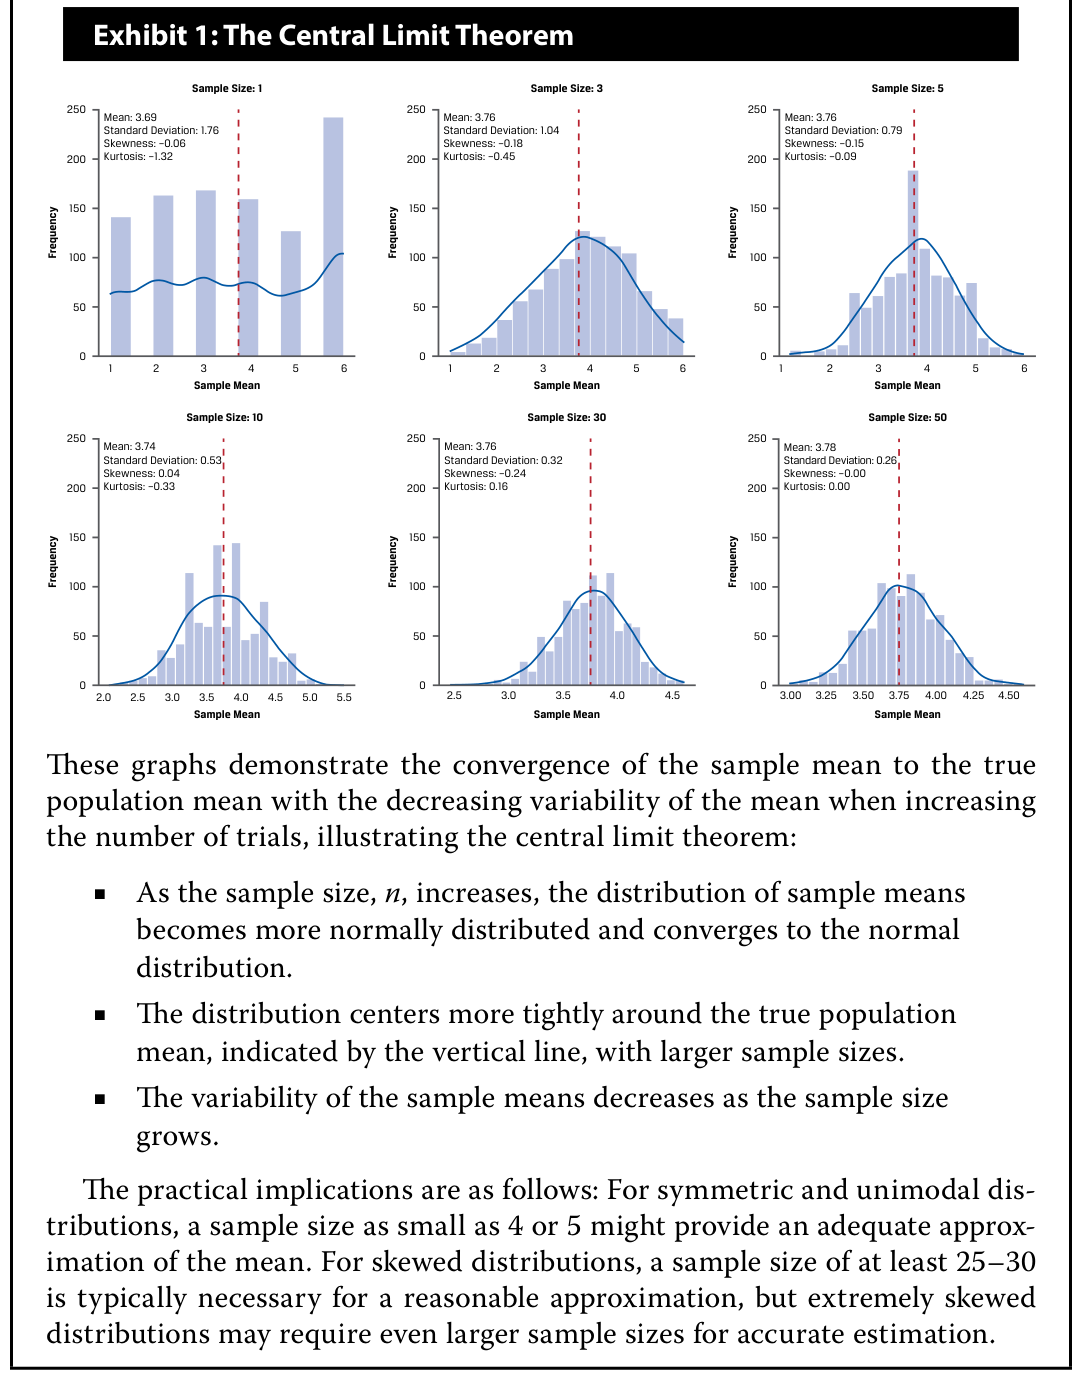
\includegraphics[width=0.85\linewidth]{002_figs/007_Module_7/exhibit_1.png}
	\caption{Histograms Showing the Convergence of the Sample Mean under CLT}
	\label{fig:mod7_exhibit_1}
\end{figure}
% Reference: CFA Curriculum 2027, Volume 1, Module 7, Page 324, Exhibit 1

An estimator $\hat{\theta}$ is:
\begin{itemize}
	\item \textbf{Unbiased} if $E[\hat{\theta}] = \theta$. The sample mean is an unbiased estimator of the population mean ($E[\bar{X}] = \mu$).
	\item \textbf{Efficient} if it has the smallest possible standard error among all unbiased estimators. A minimum-variance unbiased estimator (MVUE) is both unbiased and efficient. The best linear unbiased estimator (BLUE) is both unbiased and maximally efficient among all linear estimators.
	\item \textbf{Consistent} if it converges to the true parameter value as the sample size increases. The sample mean $\bar{X}$ is a consistent estimator.
	\item \textbf{Robust} if it provides accurate parameter estimates even when the data include outliers or violate distribution assumptions (e.g., using trimmed means).
\end{itemize}

\subsection{Confidence Intervals}
Confidence intervals are probabilistic ranges that are likely to contain the true parameter value with a specified level of confidence ($1 - \alpha$). For large sample sizes, the confidence interval for the population mean $\mu$ is:
\begin{equation}
	\bar{X} \pm Z_{\alpha/2} \times \frac{\sigma}{\sqrt{n}}
	\label{eq:confidence_interval_z_m7}
\end{equation}
% Reference: CFA Curriculum 2027, Volume 1, Module 7, Page 325, Equation (4)

Where $Z_{\alpha/2}$ is the critical Z-score from the normal distribution, and $\sigma/\sqrt{n}$ is the standard error. Exhibit~\ref{fig:mod7_exhibit_2} illustrates the normal distribution curve and confidence intervals.

\begin{figure}[!htbp]
	\centering
	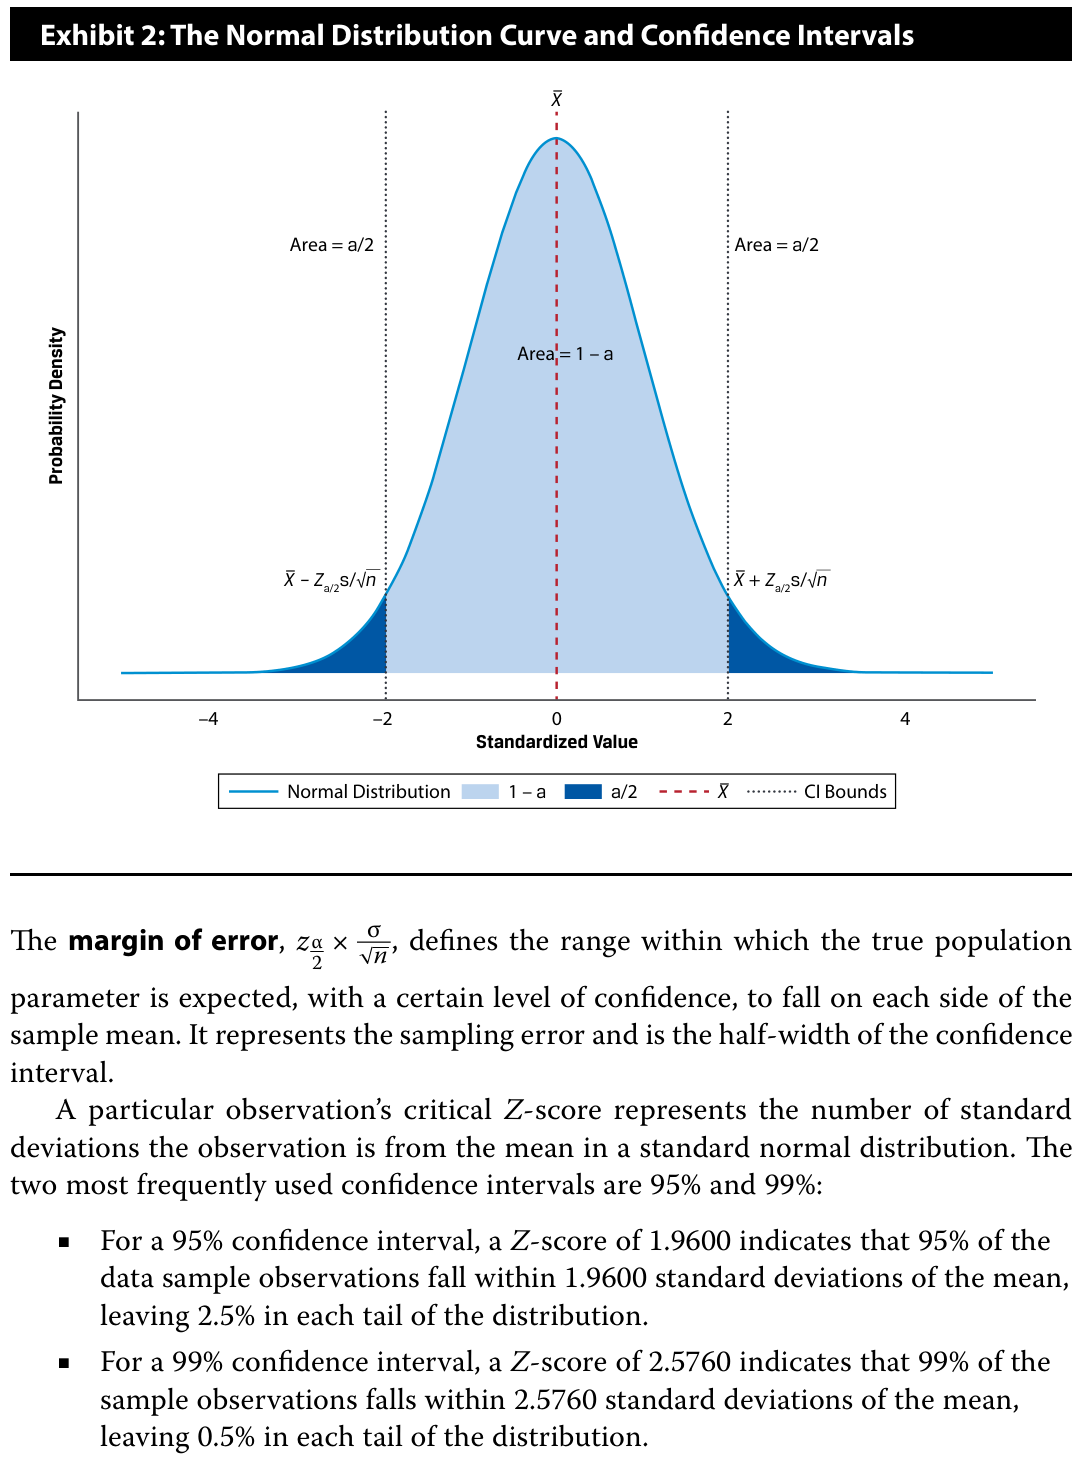
\includegraphics[width=0.75\linewidth]{002_figs/007_Module_7/exhibit_2.png}
	\caption{The Normal Distribution Curve and Confidence Intervals}
	\label{fig:mod7_exhibit_2}
\end{figure}
% Reference: CFA Curriculum 2027, Volume 1, Module 7, Page 326, Exhibit 2

The margin of error, $Z_{\alpha/2} \times \frac{\sigma}{\sqrt{n}}$, is the half-width of the confidence interval. The two most frequently used confidence intervals are:
\begin{itemize}
	\item \textbf{95\% Confidence Interval:} $Z_{0.025} = 1.9600$, leaving 2.5\% in each tail.
	\item \textbf{99\% Confidence Interval:} $Z_{0.005} = 2.5760$, leaving 0.5\% in each tail.
\end{itemize}

\begin{tcolorbox}[
	colback=gray!5!white,
	colframe=black!15!white,
	boxrule=0.5pt,
	arc=3pt,
	title=\textbf{Case Study: Estimating the Monthly Return on Gold},
	coltitle=black,
	colbacktitle=black!5!white,
	before skip=6pt,
	after skip=6pt,
	breakable
]
Based on 34 years of monthly returns on gold ($n = 408$), the average monthly return is $0.49\%$ and the sample standard deviation is $4.38\%$.
\begin{enumerate}
	\item \textbf{Standard Error:} $SE = \frac{s}{\sqrt{n}} = \frac{0.0438}{\sqrt{408}} \approx 0.0022$ (or $0.22\%$).
	\item \textbf{95\% Confidence Interval:} $0.49\% \pm 1.9600 \times 0.22\% = 0.49\% \pm 0.43\% \implies [0.06\%, 0.92\%]$.
	\item \textbf{99\% Confidence Interval:} $0.49\% \pm 2.5760 \times 0.22\% = 0.49\% \pm 0.57\% \implies [-0.08\%, 1.06\%]$.
\end{enumerate}
These intervals are shown in Exhibit~\ref{fig:mod7_exhibit_3}. Higher confidence levels result in wider confidence intervals.
\end{tcolorbox}

\begin{figure}[!htbp]
	\centering
	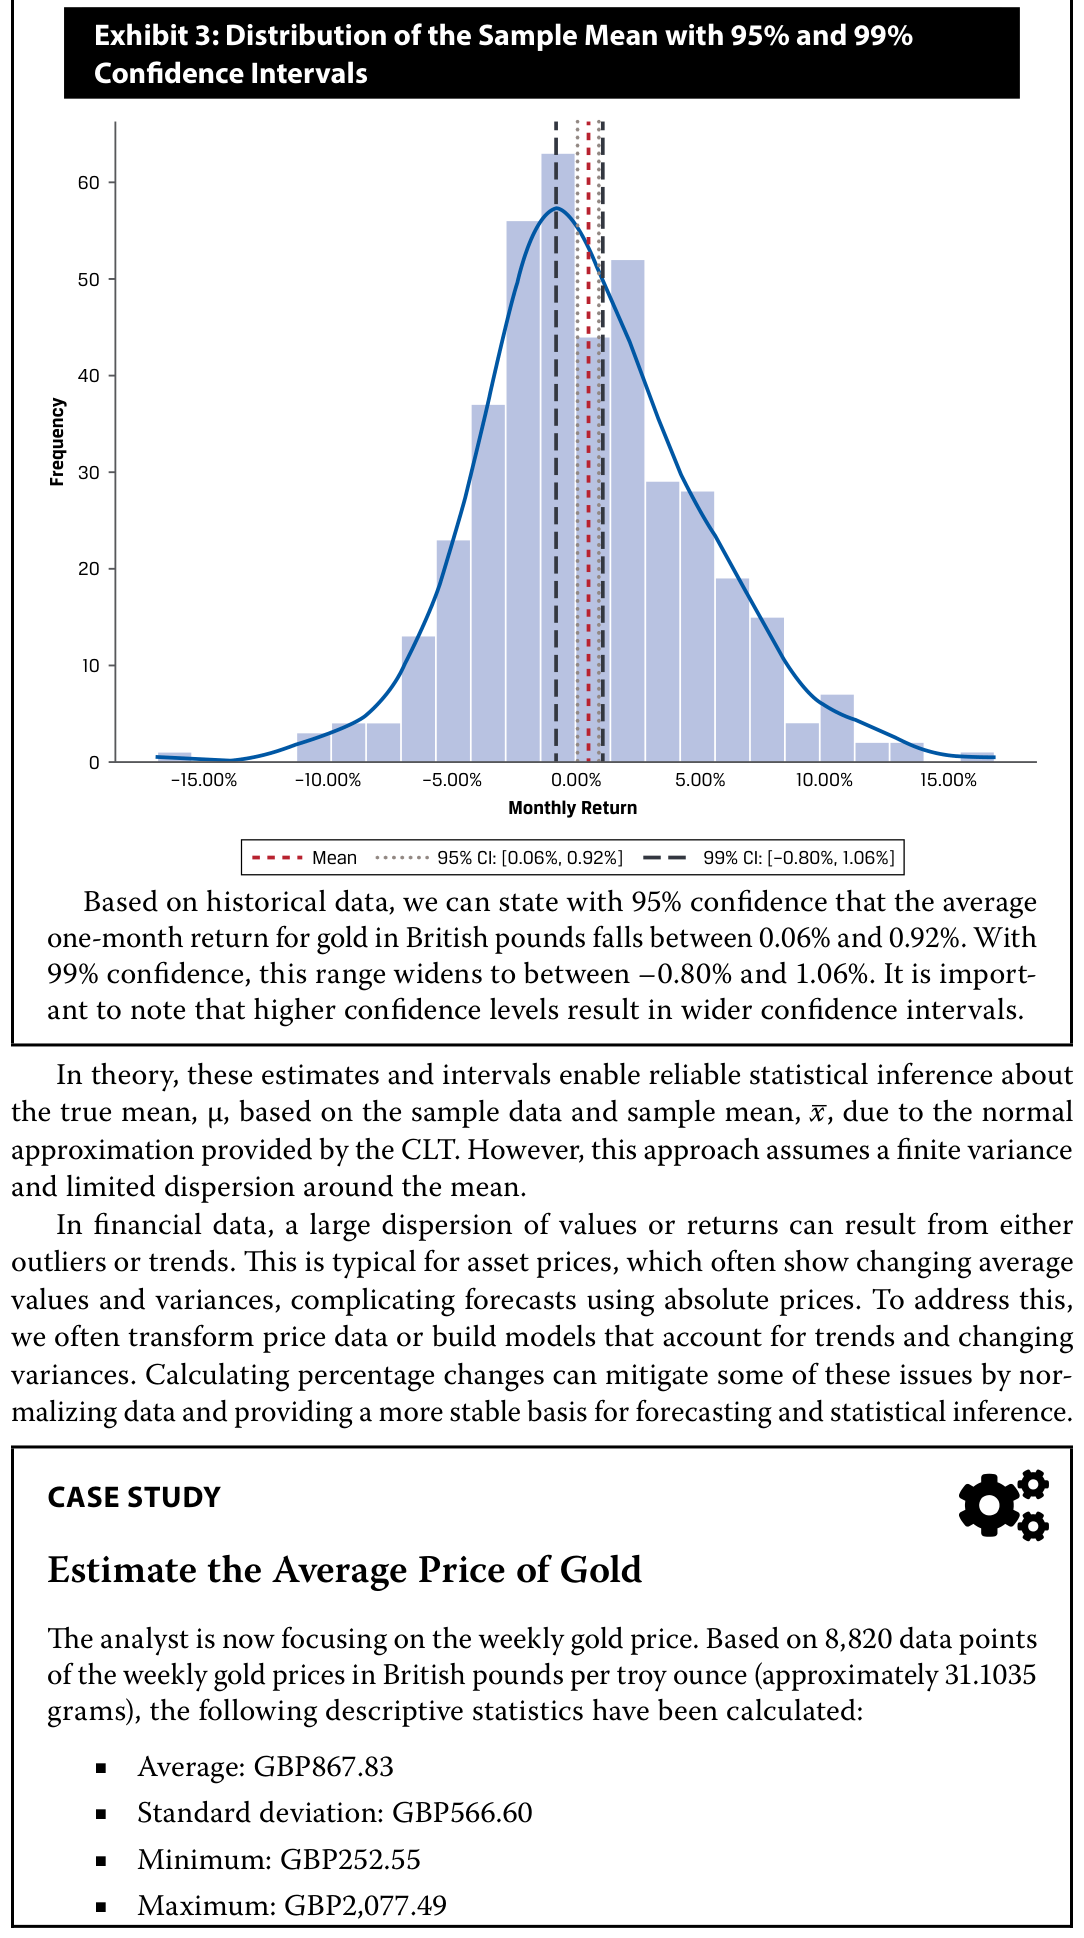
\includegraphics[width=0.75\linewidth]{002_figs/007_Module_7/exhibit_3.png}
	\caption{Distribution of the Sample Mean with 95\% and 99\% Confidence Intervals}
	\label{fig:mod7_exhibit_3}
\end{figure}
% Reference: CFA Curriculum 2027, Volume 1, Module 7, Page 328, Exhibit 3

\begin{tcolorbox}[
	colback=gray!5!white,
	colframe=black!15!white,
	boxrule=0.5pt,
	arc=3pt,
	title=\textbf{Case Study: Estimating the Average Price of Gold},
	coltitle=black,
	colbacktitle=black!5!white,
	before skip=6pt,
	after skip=6pt,
	breakable
]
Based on 8,820 weekly gold price data points, the average is GBP 867.83 and standard deviation is GBP 566.60 (Exhibit~\ref{fig:mod7_exhibit_4}). The distribution of prices is bimodal and highly skewed. This violates the normal distribution assumption of the CLT, making absolute price confidence intervals unreliable. Thus, transforming data into returns (percentage changes) is necessary to stabilize the variance.
\end{tcolorbox}

\begin{figure}[!htbp]
	\centering
	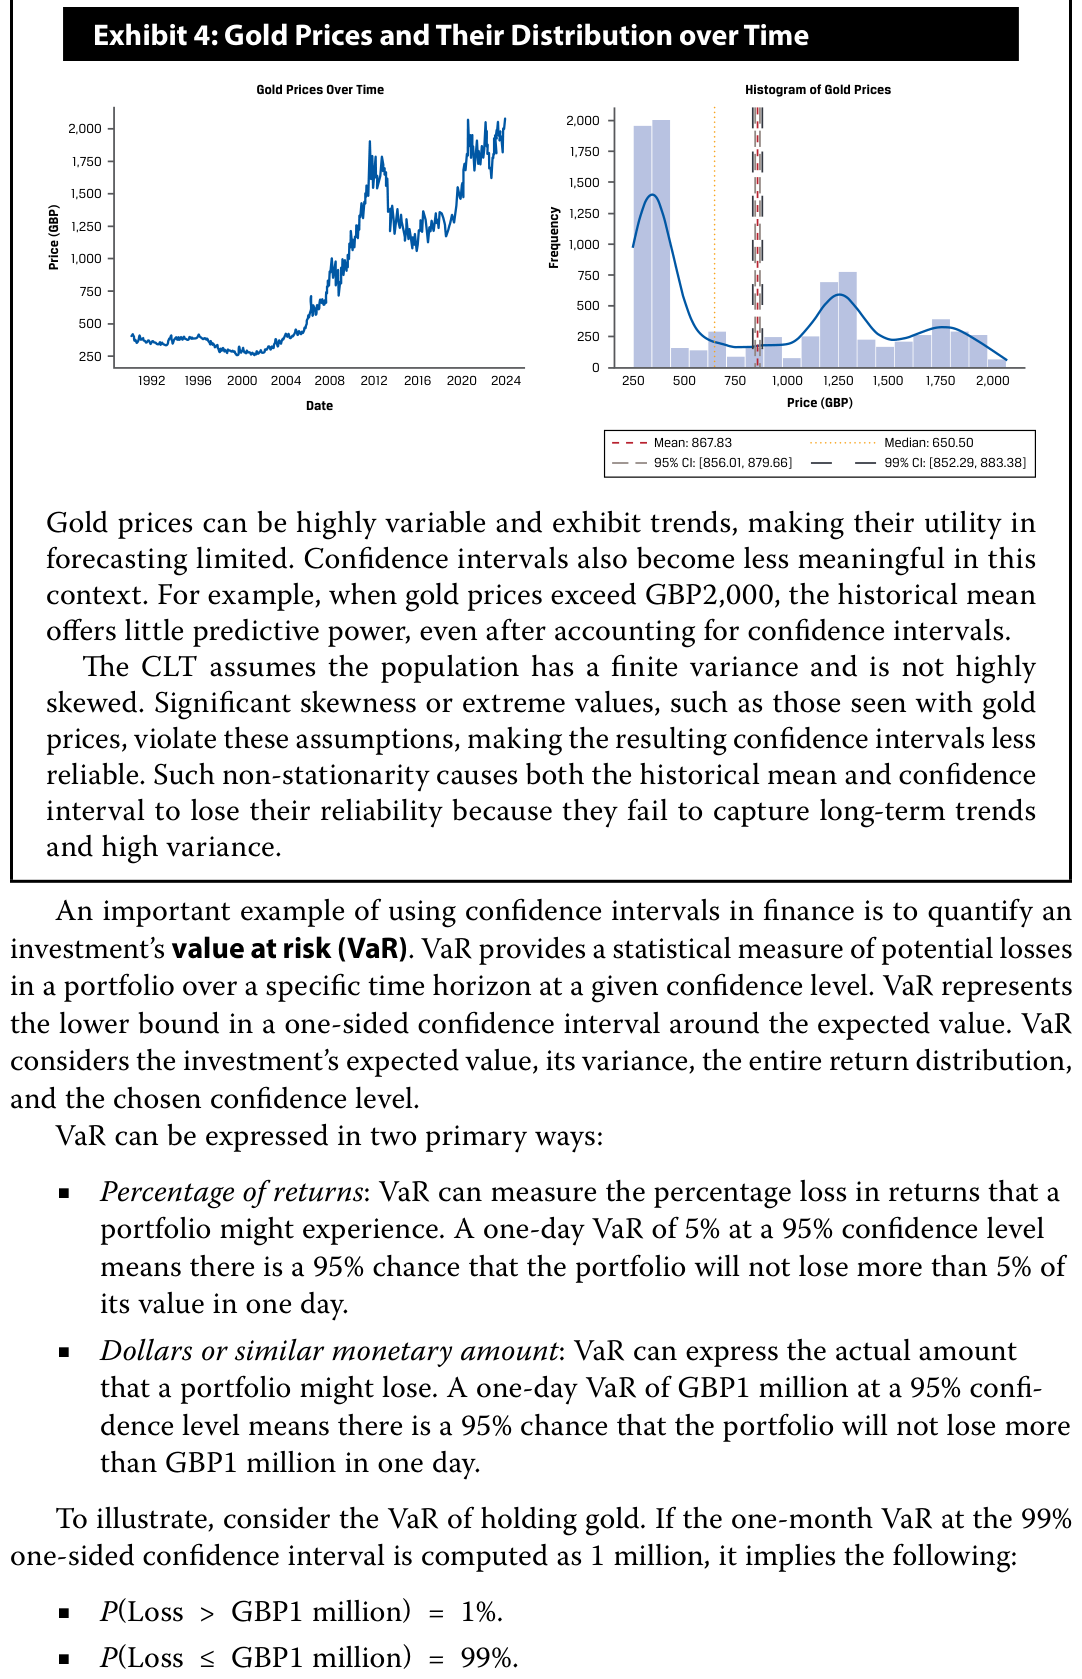
\includegraphics[width=0.85\linewidth]{002_figs/007_Module_7/exhibit_4.png}
	\caption{Gold Prices and Their Bimodal Distribution over Time}
	\label{fig:mod7_exhibit_4}
\end{figure}
% Reference: CFA Curriculum 2027, Volume 1, Module 7, Page 329, Exhibit 4

\begin{examtip}
\textbf{Value at Risk (VaR) as a One-Sided Confidence Interval}\\
VaR provides a statistical measure of potential losses in a portfolio over a specific time horizon at a given confidence level. It represents the lower bound of a one-sided confidence interval.
\begin{itemize}
	\item $P(\text{Loss} > \text{VaR}) = \alpha$
	\item $P(\text{Loss} \le \text{VaR}) = 1 - \alpha$
\end{itemize}
Assuming normally distributed asset returns and a mean return of zero, the parametric VaR is:
\begin{equation}
	\text{VaR} = Z_{\alpha} \times \sigma \times P
	\label{eq:var_formula_m7}
\end{equation}
% Reference: CFA Curriculum 2027, Volume 1, Module 7, Page 330, Equation (5)
Where $Z_{\alpha}$ corresponds to the one-sided percentile (e.g., $1.65$ for 95\%, $2.33$ for 99\%), $\sigma$ is standard deviation, and $P$ is the current position value (Exhibit~\ref{fig:mod7_exhibit_5}).
\end{examtip}

\begin{figure}[!htbp]
	\centering
	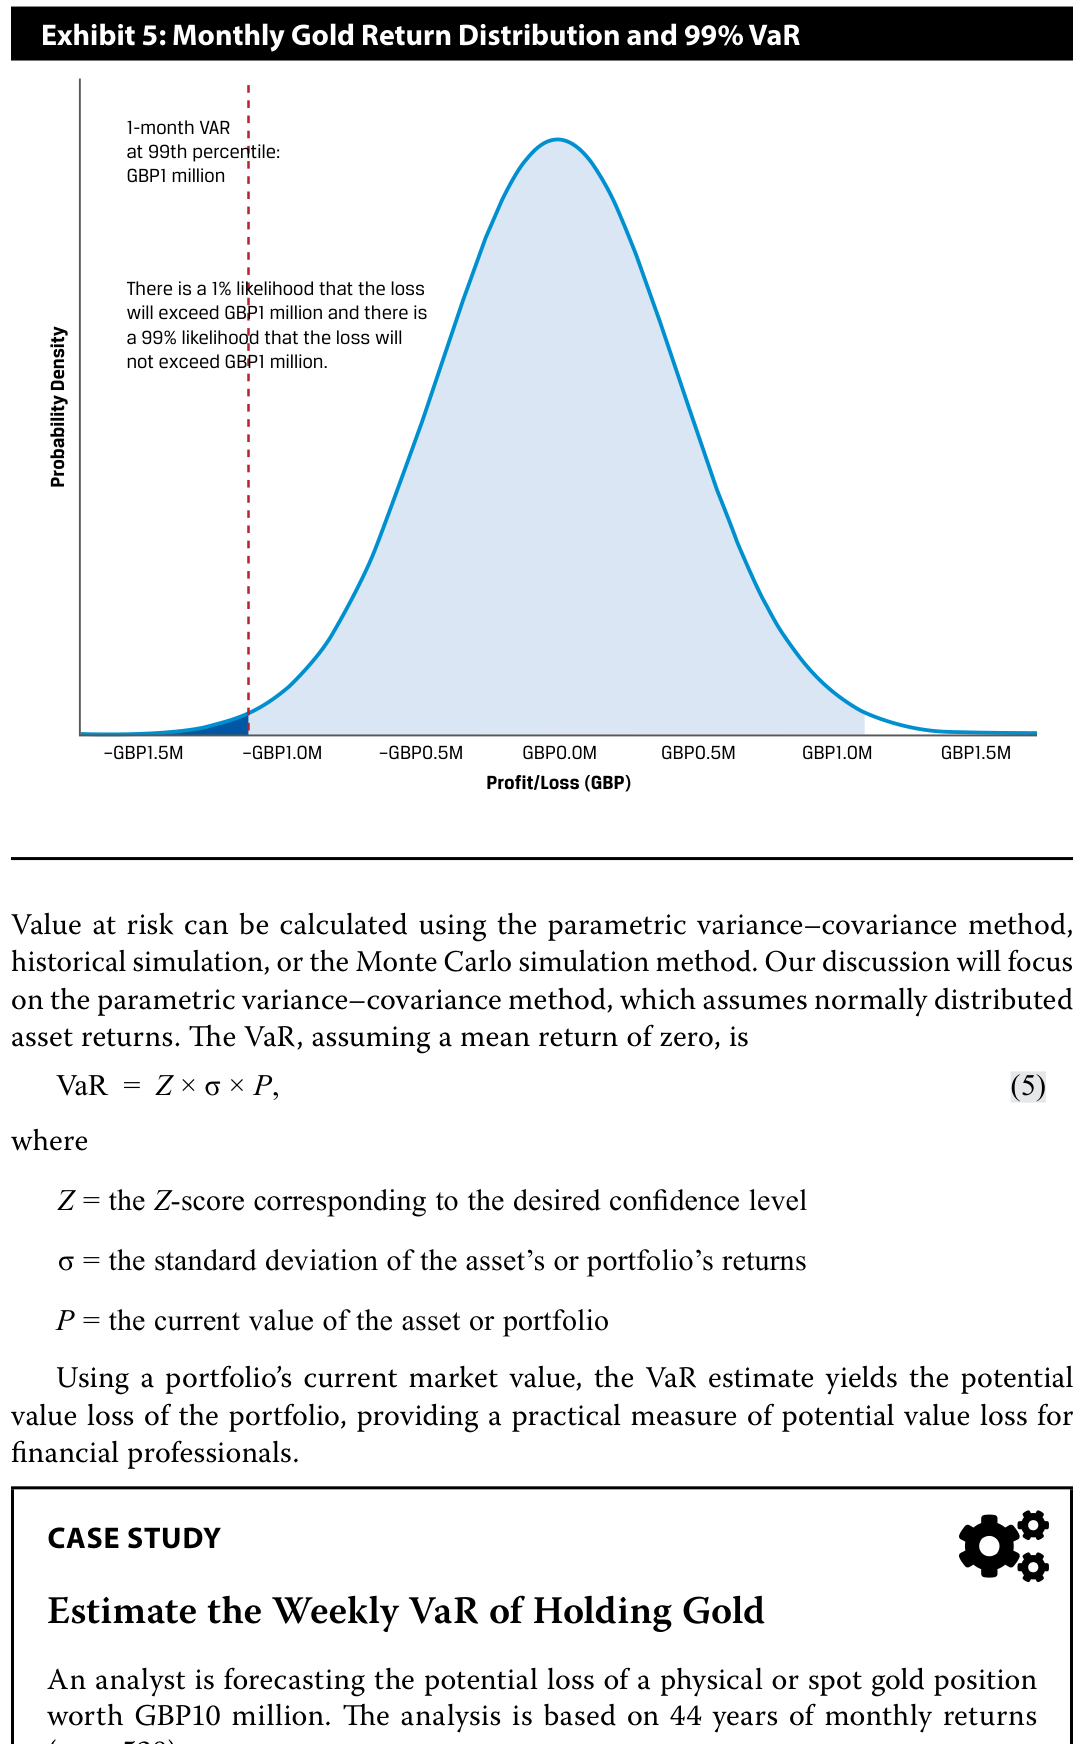
\includegraphics[width=0.75\linewidth]{002_figs/007_Module_7/exhibit_5.png}
	\caption{Monthly Gold Return Distribution and 99\% VaR}
	\label{fig:mod7_exhibit_5}
\end{figure}
% Reference: CFA Curriculum 2027, Volume 1, Module 7, Page 330, Exhibit 5

\begin{tcolorbox}[
	colback=gray!5!white,
	colframe=black!15!white,
	boxrule=0.5pt,
	arc=3pt,
	title=\textbf{Case Study: Estimating the Weekly VaR of Gold},
	coltitle=black,
	colbacktitle=black!5!white,
	before skip=6pt,
	after skip=6pt,
	breakable
]
An analyst forecasts potential loss of a spot gold position worth GBP 10 million. Monthly standard deviation is $5.02\%$. Assuming a mean return of 0\% and normal distribution, the 99\% one-month VaR is:
\[ \text{VaR} = 2.33 \times 5.02\% \times \text{GBP } 10,000,000 = \text{GBP } 1,169,660 \]
There is a 1\% probability that the position will lose more than GBP 1,169,660 over the next month.
\end{tcolorbox}

\subsection{Sampling Methodologies}
To extract information about a population, two sampling approaches can be used:
\begin{enumerate}
	\item \textbf{Probability Sampling:} Every member of the population has a known, non-zero chance of selection.
	      \begin{itemize}
		      \item \textbf{Simple Random Sampling:} Each element has an equal selection chance.
		      \item \textbf{Systematic Sampling:} Selects every $k$-th member of a population.
		      \item \textbf{Stratified Random Sampling:} Divides the population into strata based on criteria, then draws random samples proportionally from each stratum. This increases precision.
		      \item \textbf{Cluster Sampling:} Divides the population into small clusters, randomly selects clusters, and samples all members in selected clusters.
	      \end{itemize}
	\item \textbf{Non-Probability Sampling:} Relies on judgment or convenience; does not guarantee representativeness, so the CLT does not reliably apply.
	      \begin{itemize}
		      \item \textbf{Convenience Sampling:} Selecting accessible elements.
		      \item \textbf{Judgmental Sampling:} Selecting elements based on expertise.
	      \end{itemize}
\end{enumerate}

\begin{tcolorbox}[
	colback=gray!5!white,
	colframe=black!15!white,
	boxrule=0.5pt,
	arc=3pt,
	title=\textbf{Case Study: Sampling of Daily Returns},
	coltitle=black,
	colbacktitle=black!5!white,
	before skip=6pt,
	after skip=6pt,
	breakable
]
Based on 1,258 daily return observations of a global small-cap stock index, the true population mean is $0.035\%$. As shown in Exhibit~\ref{fig:mod7_exhibit_6}, mean absolute errors decrease rapidly as sample size $n$ increases. Stratified sampling (stratified by year) generally yields smaller errors than simple random sampling, although the advantage decreases as sample size grows.
\end{tcolorbox}

\begin{figure}[!htbp]
	\centering
	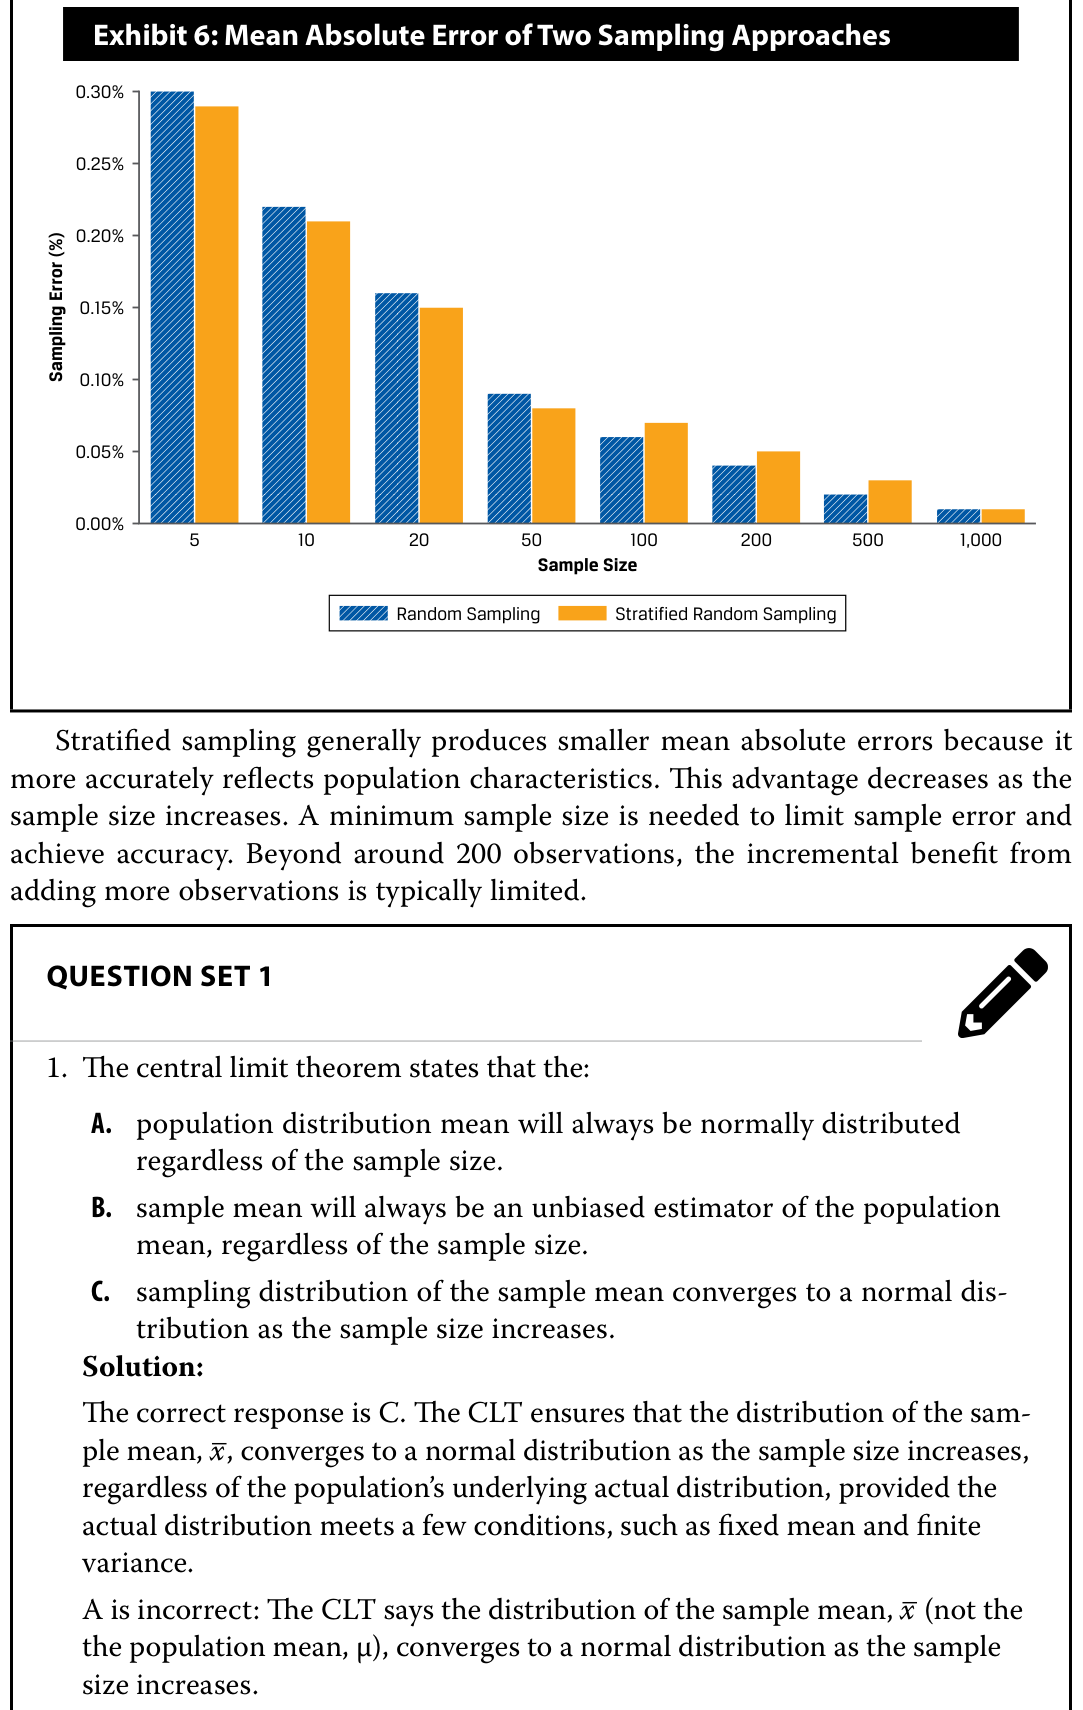
\includegraphics[width=0.75\linewidth]{002_figs/007_Module_7/exhibit_6.png}
	\caption{Mean Absolute Error of Random vs Stratified Sampling}
	\label{fig:mod7_exhibit_6}
\end{figure}
% Reference: CFA Curriculum 2027, Volume 1, Module 7, Page 334, Exhibit 6

\section{HYPOTHESIS TESTING AND PARAMETRIC TESTING}
\begin{center}
\begin{tabular}{p{0.06\linewidth} | p{0.88\linewidth}}
	b & explain hypothesis testing and its components, including statistical significance, Type I and Type II errors, and the power of a test; construct appropriate hypothesis tests; and interpret the results \\
\end{tabular}
\end{center}

\textcolor{blue}{\textit{Quy trình kiểm định giả thuyết gồm 4 bước (Exhibit~\ref{fig:mod7_exhibit_7}). Chúng ta đặc biệt lưu ý lỗi Loại I ($\alpha$ - bác bỏ $H_0$ đúng), lỗi Loại II ($\beta$ - không bác bỏ $H_0$ sai) và lực lượng kiểm định ($1 - \beta$). Nhớ phân phối tương ứng: kiểm định trung bình ($t$), một phương sai ($\chi^2$), hai phương sai ($F$).}}

\subsection{The Hypothesis Testing Process}
Hypothesis testing involves four steps, as outlined in Exhibit~\ref{fig:mod7_exhibit_7}:
\begin{enumerate}
	\item State the null hypothesis ($H_0$) and alternative hypothesis ($H_A$).
	\item Identify the test statistic and its probability distribution.
	\item Specify the level of significance ($\alpha$).
	\item Establish the decision rule, calculate the statistic, and make the decision.
\end{enumerate}

\begin{figure}[!htbp]
	\centering
	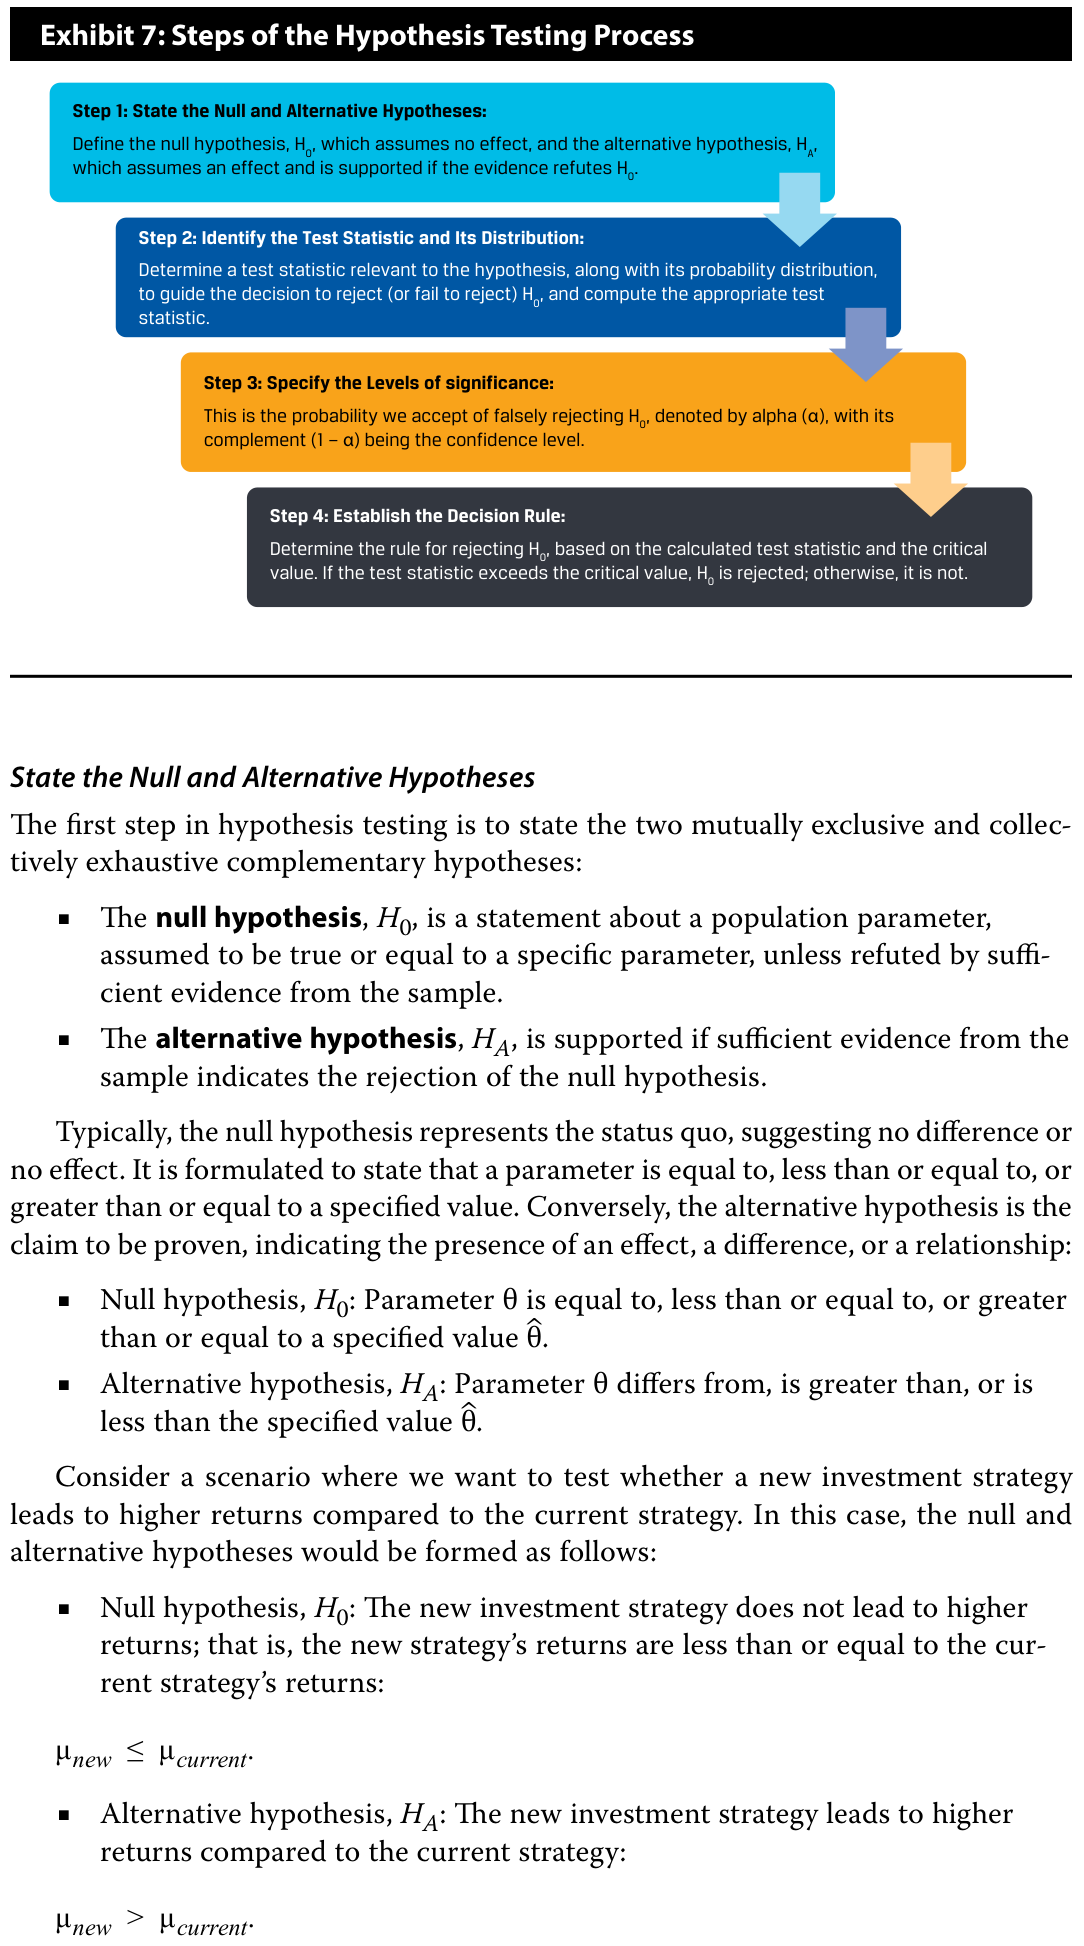
\includegraphics[width=0.7\linewidth]{002_figs/007_Module_7/exhibit_7.png}
	\caption{Steps of the Hypothesis Testing Process}
	\label{fig:mod7_exhibit_7}
\end{figure}
% Reference: CFA Curriculum 2027, Volume 1, Module 7, Page 337, Exhibit 7

\begin{figure}[!htbp]
	\centering
	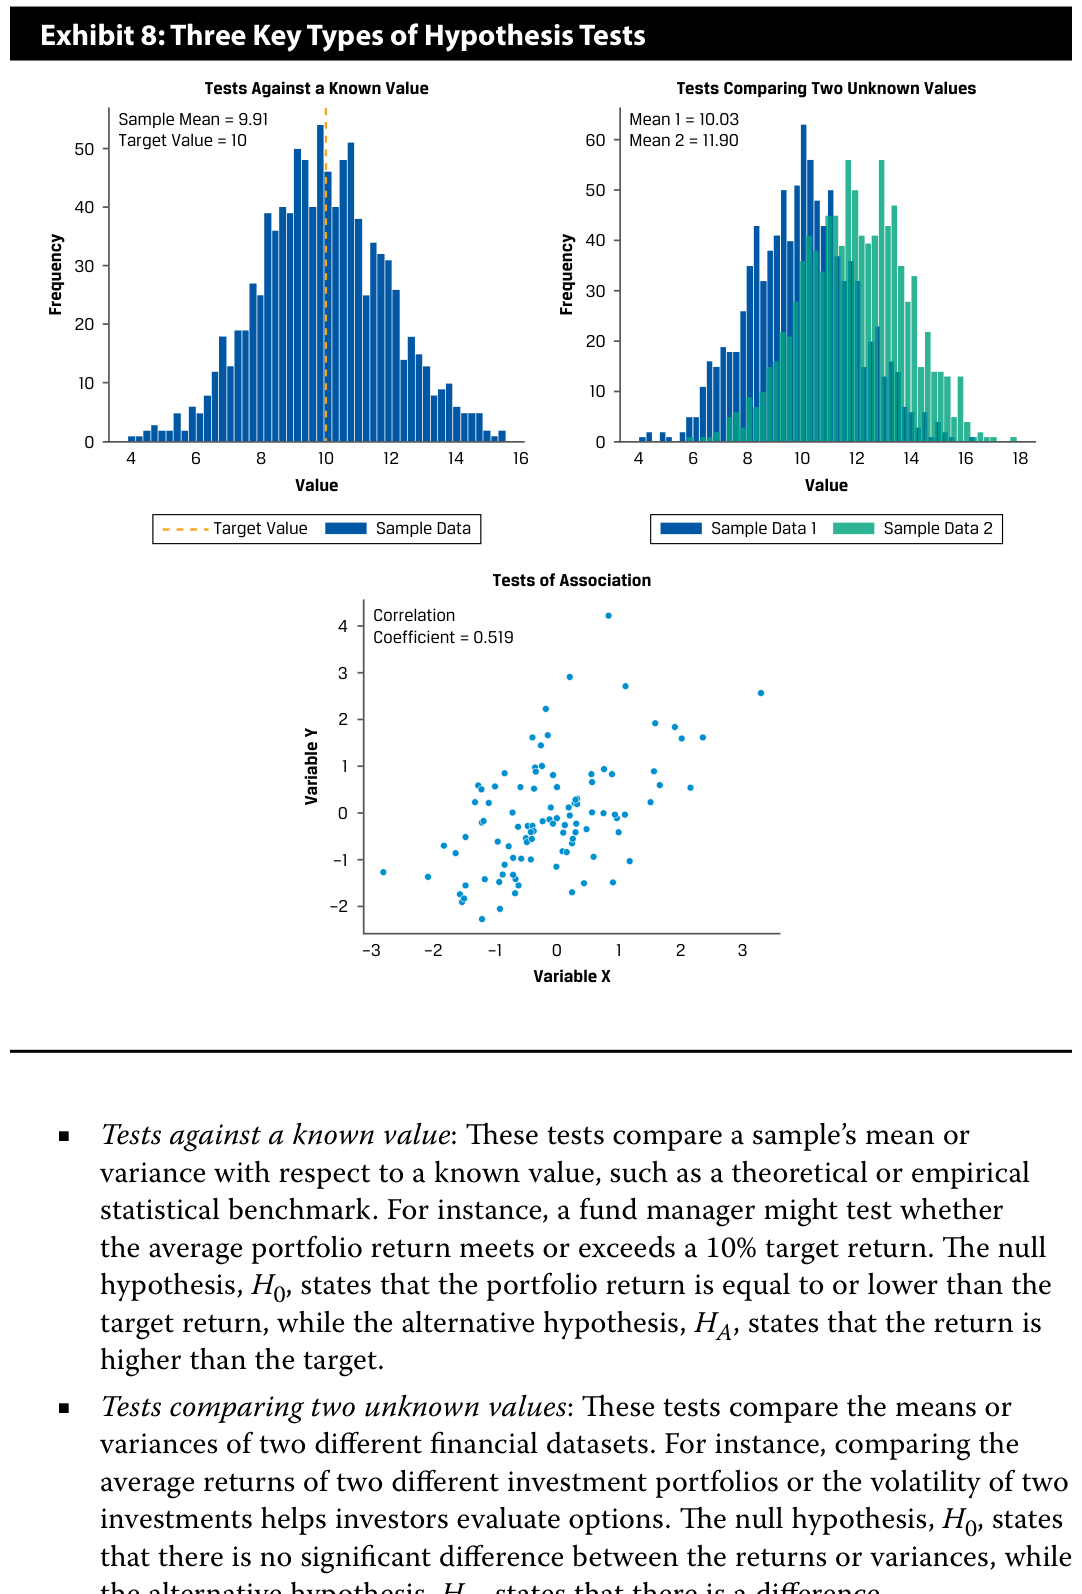
\includegraphics[width=0.75\linewidth]{002_figs/007_Module_7/exhibit_8.png}
	\caption{Three Key Types of Hypothesis Tests}
	\label{fig:mod7_exhibit_8}
\end{figure}
% Reference: CFA Curriculum 2027, Volume 1, Module 7, Page 338, Exhibit 8

Hypothesis tests can be formulated in three ways (Exhibit~\ref{fig:mod7_exhibit_8} \& Exhibit~\ref{tab:hypotheses_types_m7}):
\begin{itemize}
	\item \textbf{Right-tail test:} Tests whether a parameter $\theta$ is significantly greater than $\theta_0$ ($H_0: \theta \le \theta_0$ vs $H_A: \theta > \theta_0$).
	\item \textbf{Left-tail test:} Tests whether a parameter $\theta$ is significantly less than $\theta_0$ ($H_0: \theta \ge \theta_0$ vs $H_A: \theta < \theta_0$).
	\item \textbf{Two-tailed test:} Tests whether a parameter $\theta$ is significantly different from $\theta_0$ ($H_0: \theta = \theta_0$ vs $H_A: \theta \ne \theta_0$).
\end{itemize}

\begin{table}[!htbp]
\centering
\caption{General Formulation of Hypotheses}
\label{tab:hypotheses_types_m7}
\begin{tabular}{p{0.20\linewidth} p{0.38\linewidth} p{0.18\linewidth} p{0.14\linewidth}}
\toprule
\textbf{Test Type} & \textbf{Null Hypothesis ($H_0$)} & \textbf{Alternative ($H_A$)} & \textbf{Rejection Region} \\
\midrule
\textbf{Right-tail test} & $\theta \le \theta_0$ & $\theta > \theta_0$ & Right tail \\
\textbf{Left-tail test} & $\theta \ge \theta_0$ & $\theta < \theta_0$ & Left tail \\
\textbf{Two-tailed test} & $\theta = \theta_0$ & $\theta \ne \theta_0$ & Both tails \\
\bottomrule
\end{tabular}
\end{table}
% Reference: CFA Curriculum 2027, Volume 1, Module 7, Page 339, Exhibit 9

Exhibit~\ref{fig:mod7_exhibit_10} depicts the rejection areas for the three types of hypothesis tests.

\begin{figure}[!htbp]
	\centering
	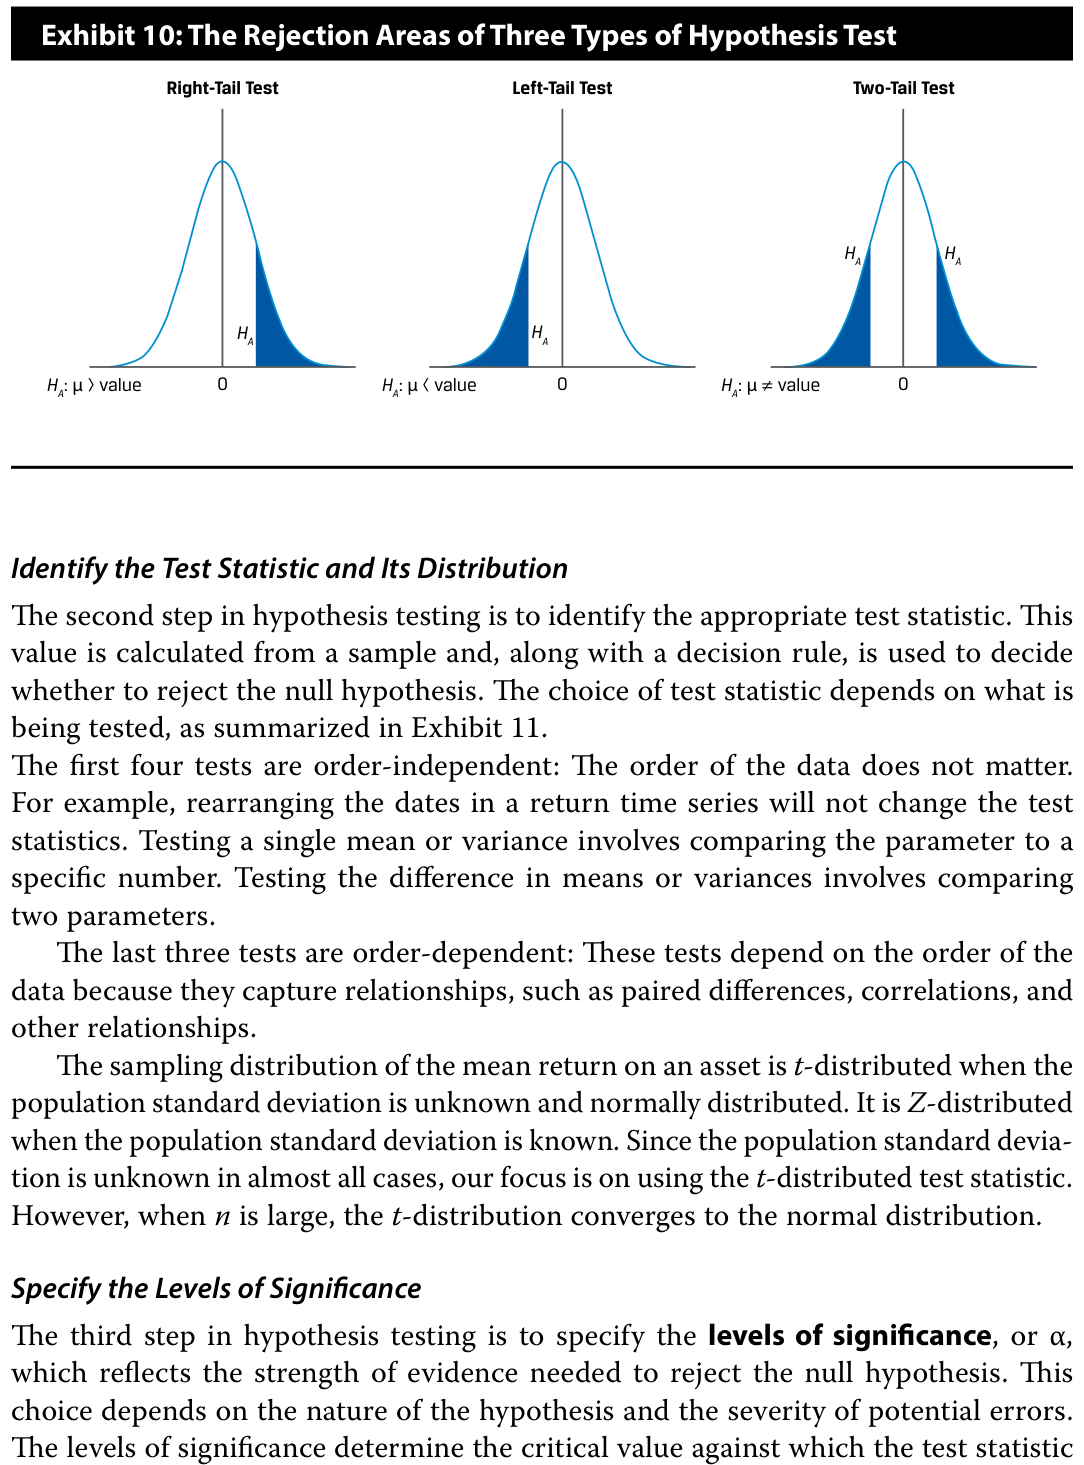
\includegraphics[width=0.85\linewidth]{002_figs/007_Module_7/exhibit_10.png}
	\caption{Rejection Regions for One-Tailed and Two-Tailed Tests}
	\label{fig:mod7_exhibit_10}
\end{figure}
% Reference: CFA Curriculum 2027, Volume 1, Module 7, Page 340, Exhibit 10

\subsection{Type I and Type II Errors}
The decision-making process in hypothesis testing involves two types of errors:
\begin{itemize}
	\item \textbf{Type I Error (False Positive):} Rejecting a true null hypothesis. The probability of a Type I error is the level of significance, $\alpha$.
	\item \textbf{Type II Error (False Negative):} Failing to reject a false null hypothesis. The probability of a Type II error is denoted by $\beta$.
\end{itemize}

\begin{table}[!htbp]
\centering
\caption{Decisions in Hypothesis Testing}
\label{tab:decision_matrix_m7}
\begin{tabular}{p{0.28\linewidth} | p{0.32\linewidth} | p{0.32\linewidth}}
\toprule
\textbf{Decision} & \textbf{Null Hypothesis ($H_0$) is True} & \textbf{Null Hypothesis ($H_0$) is False} \\
\midrule
\textbf{Fail to reject $H_0$} & Correct Decision ($1 - \alpha$) & Type II Error ($\beta$, False Negative) \\
\midrule
\textbf{Reject $H_0$} & Type I Error ($\alpha$, False Positive) & Correct Decision ($1 - \beta$, Power of the Test) \\
\bottomrule
\end{tabular}
\end{table}
% Reference: CFA Curriculum 2027, Volume 1, Module 7, Page 342, Exhibit 12

The relation between $\alpha$ and $\beta$ is shown in Exhibit~\ref{fig:mod7_exhibit_13}. Reducing $\alpha$ increases $\beta$ for a fixed sample size. To decrease both errors simultaneously, we must increase the sample size $n$.

\begin{figure}[!htbp]
	\centering
	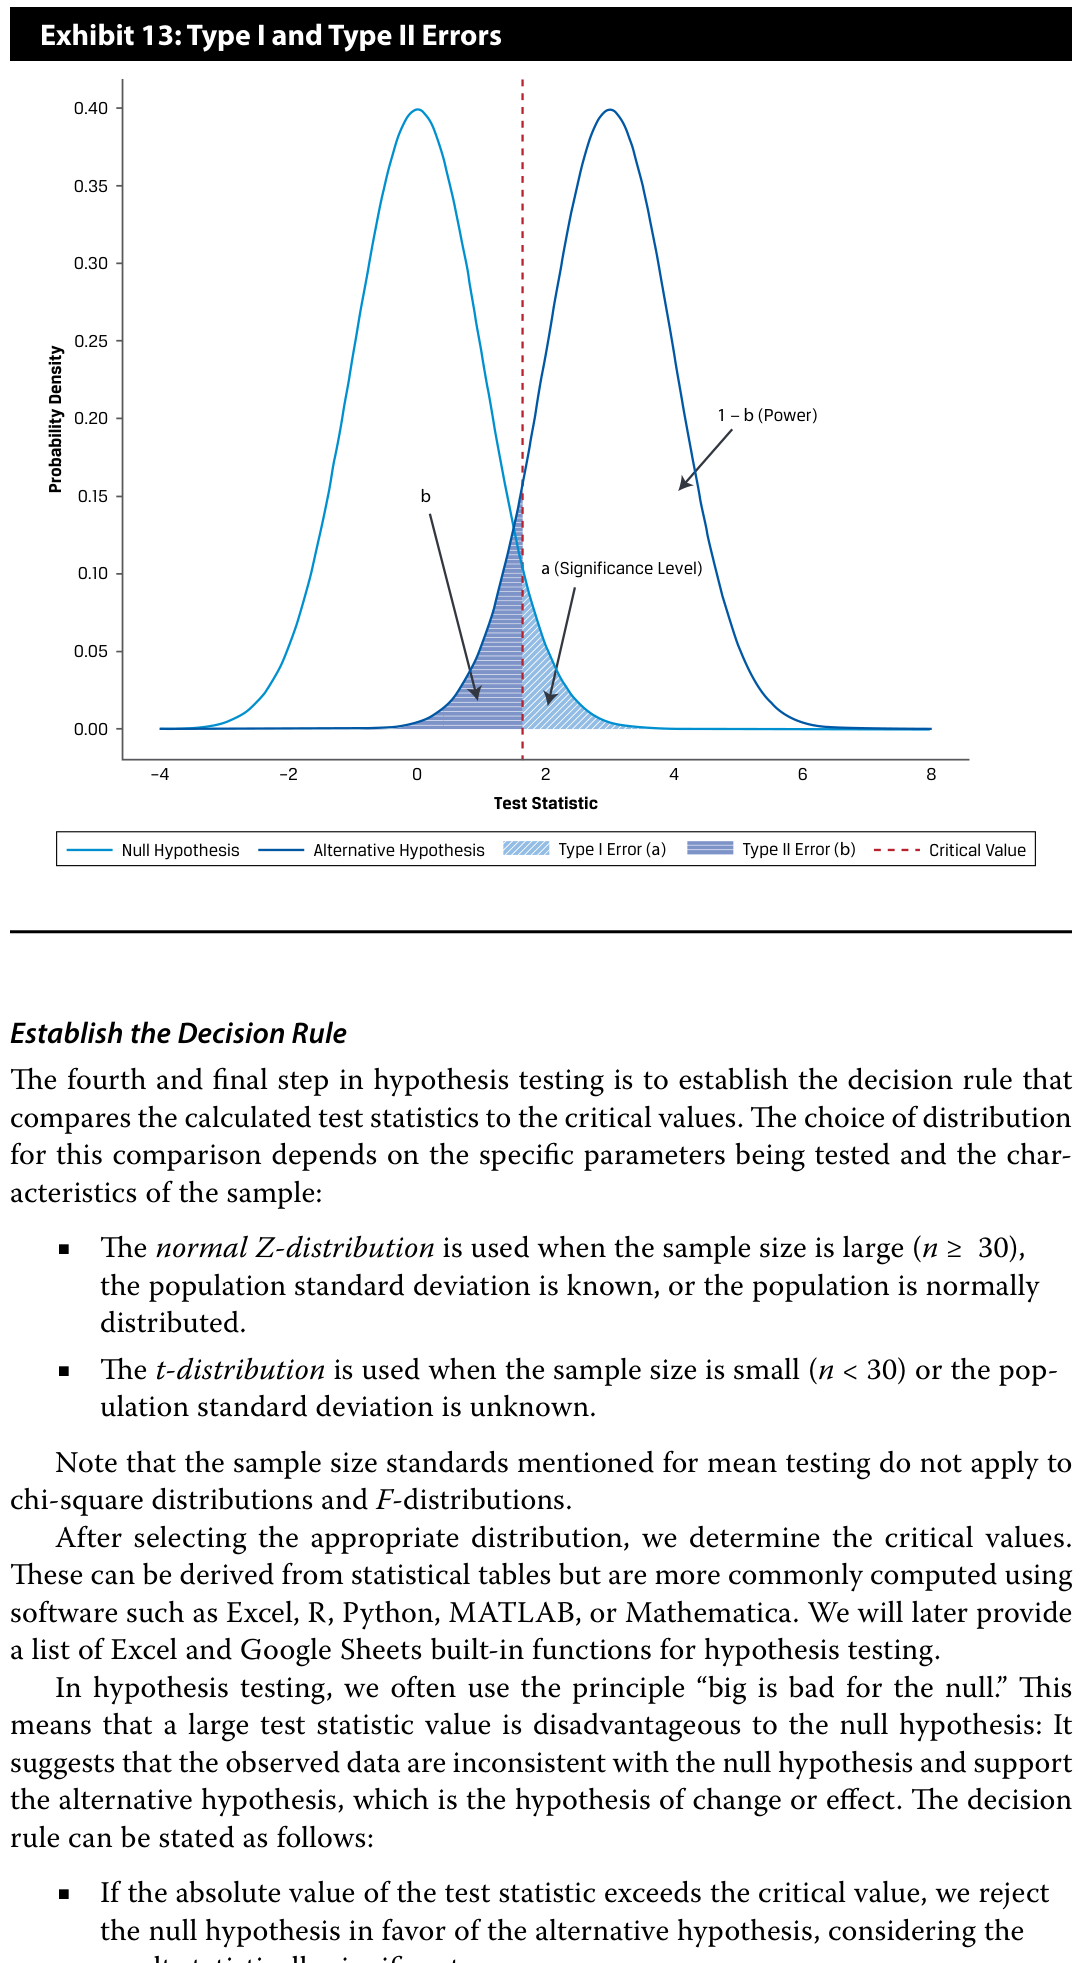
\includegraphics[width=0.75\linewidth]{002_figs/007_Module_7/exhibit_13.png}
	\caption{The Trade-Off Between Type I and Type II Errors}
	\label{fig:mod7_exhibit_13}
\end{figure}
% Reference: CFA Curriculum 2027, Volume 1, Module 7, Page 343, Exhibit 13

\subsection{Parametric Tests for a Single Variable}
We utilize annual return data from 1979 to 2023 ($n = 44$) for the MSCI World Value and Growth Indexes to illustrate parametric tests (Exhibit~\ref{fig:mod7_exhibit_14} \& Table~\ref{tab:msci_stats_m7}).

\begin{figure}[!htbp]
	\centering
	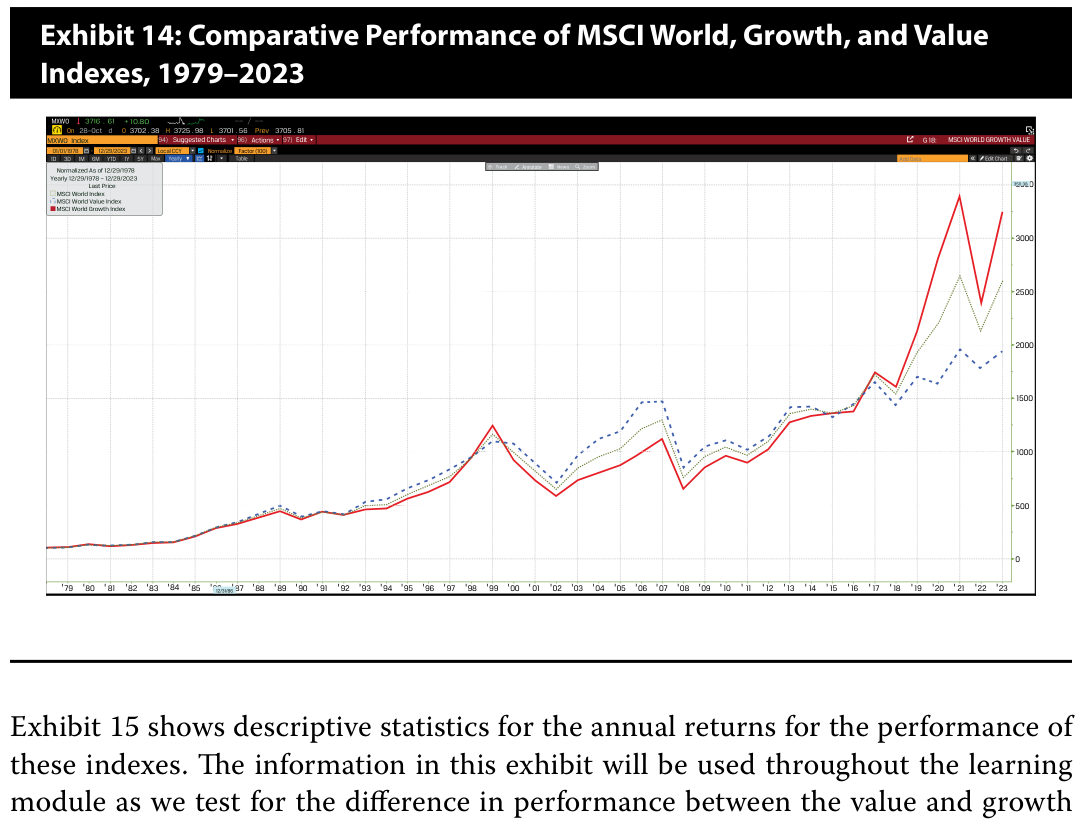
\includegraphics[width=0.85\linewidth]{002_figs/007_Module_7/exhibit_14.png}
	\caption{Performance of MSCI World, Growth, and Value Indexes, 1979--2023}
	\label{fig:mod7_exhibit_14}
\end{figure}
% Reference: CFA Curriculum 2027, Volume 1, Module 7, Page 345, Exhibit 14

\begin{table}[!htbp]
\centering
\caption{Descriptive Statistics for MSCI World, Value, and Growth Indexes}
\label{tab:msci_stats_m7}
\begin{tabular}{p{0.40\linewidth} p{0.16\linewidth} p{0.14\linewidth} p{0.15\linewidth}}
\toprule
\textbf{Metric} & \textbf{MSCI World} & \textbf{Growth Index} & \textbf{Value Index} \\
\midrule
Average annual return ($\bar{X}$) & 7.91\% & 8.81\% & 7.17\% \\
Sample variance ($s^2$) & 0.0381 & 0.0456 & 0.0362 \\
Sample standard deviation ($s$) & 0.1952 & 0.2134 & 0.1902 \\
Number of observations ($n$) & 44 & 44 & 44 \\
\bottomrule
\end{tabular}
\end{table}
% Reference: CFA Curriculum 2027, Volume 1, Module 7, Page 346, Exhibit 15

\subsubsection{Test of a Single Mean}
When the population standard deviation is unknown, the $t$-test statistic with $n - 1$ degrees of freedom is:
\begin{equation}
	t = \frac{\bar{X} - \mu_0}{s / \sqrt{n}}
	\label{eq:single_mean_t_test_m7}
\end{equation}
% Reference: CFA Curriculum 2027, Volume 1, Module 7, Page 346, Equation (6)

\begin{tcolorbox}[
	colback=gray!5!white,
	colframe=black!15!white,
	boxrule=0.5pt,
	arc=3pt,
	title=\textbf{Case Study: Testing MSCI World Value Index Mean Return},
	coltitle=black,
	colbacktitle=black!5!white,
	before skip=6pt,
	after skip=6pt,
	breakable
]
We test whether the average return of global value stocks is greater than zero ($H_0: \mu \le 0$ vs $H_A: \mu > 0$).
\begin{enumerate}
	\item \textbf{Calculate Test Statistic:} $t = \frac{0.0717 - 0}{0.1902 / \sqrt{44}} \approx 2.5001$.
	\item \textbf{Decision Rule ($df = 43$):} One-tailed critical values are $t_{0.05} = 1.6811$ and $t_{0.01} = 2.4163$ (Exhibit~\ref{fig:mod7_exhibit_16}).
	\item \textbf{Conclusion:} Since $2.5001 > 2.4163$, we reject $H_0$ at both the 5\% and 1\% levels. The average return is significantly greater than zero.
\end{enumerate}
\end{tcolorbox}

\begin{figure}[!htbp]
	\centering
	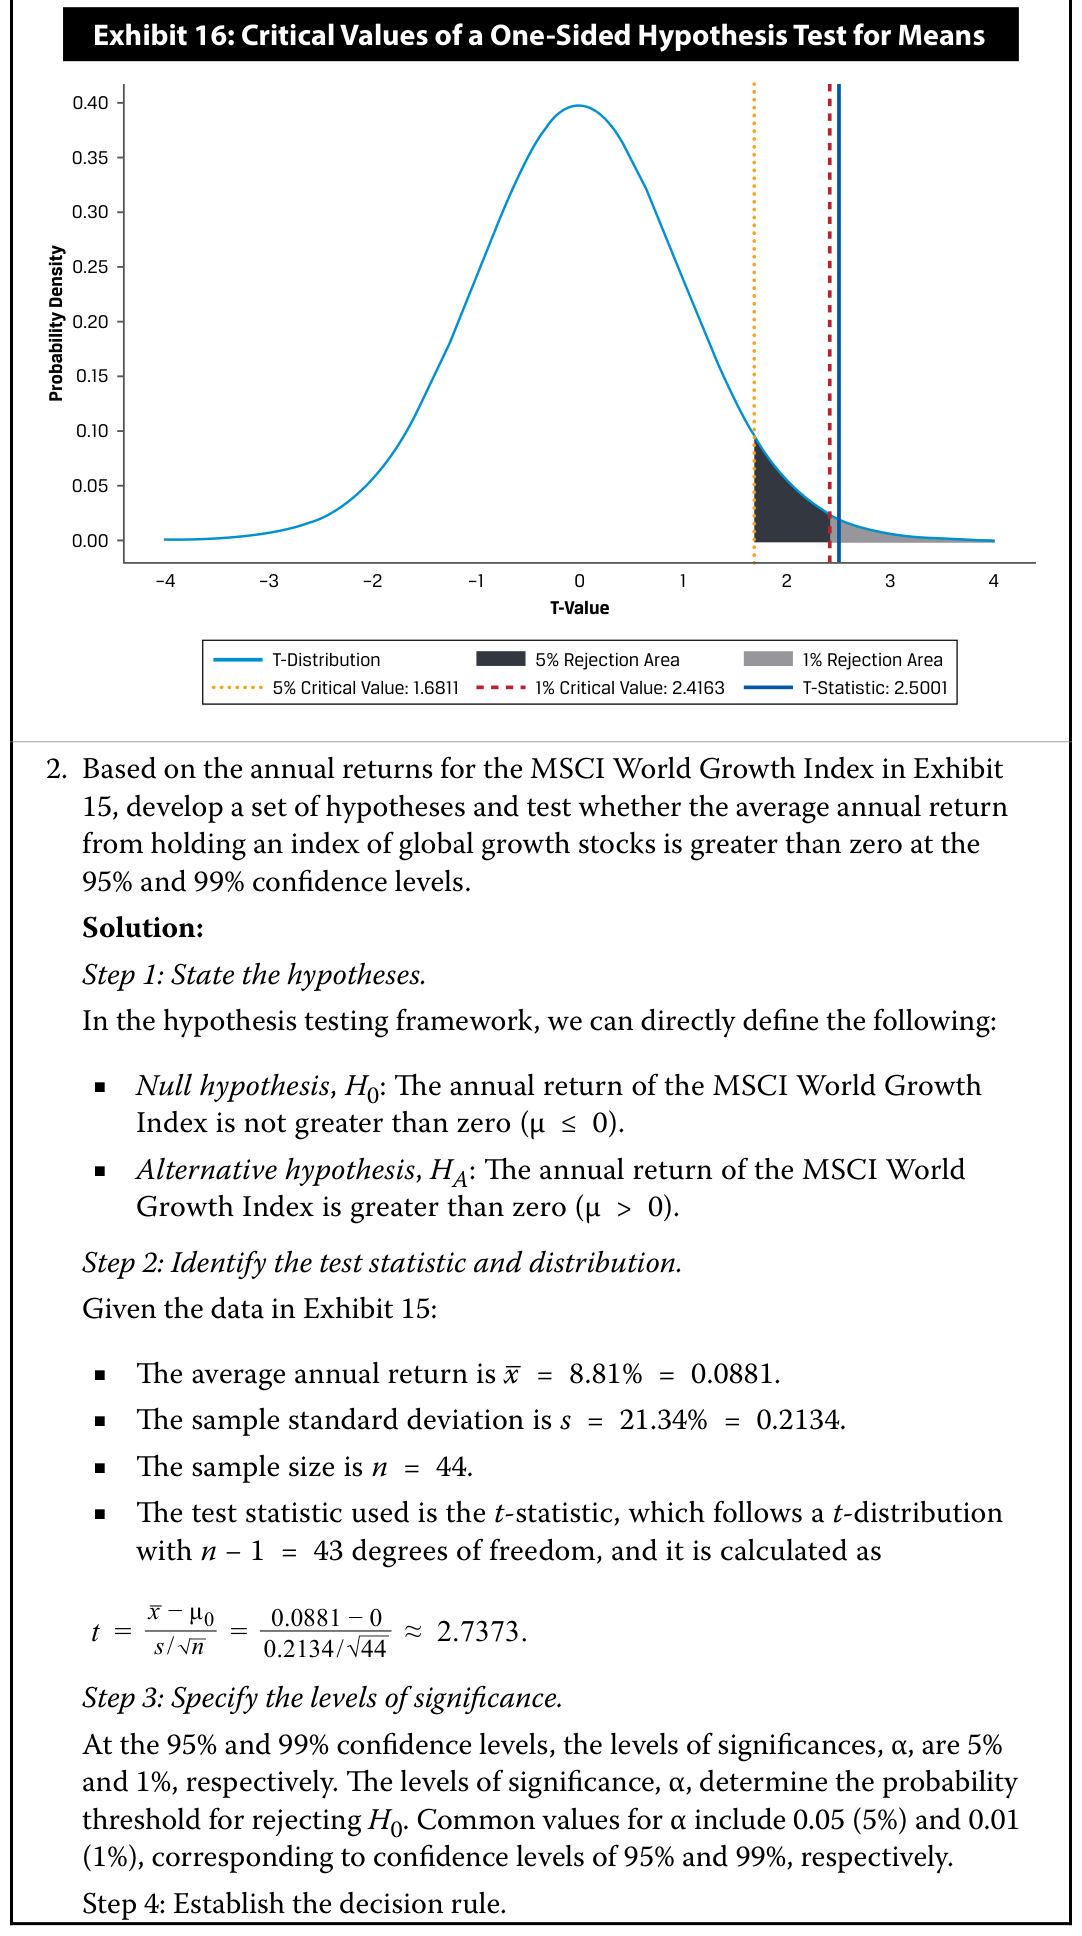
\includegraphics[width=0.75\linewidth]{002_figs/007_Module_7/exhibit_16.png}
	\caption{One-Sided Mean Test Critical Values and Rejection Regions}
	\label{fig:mod7_exhibit_16}
\end{figure}
% Reference: CFA Curriculum 2027, Volume 1, Module 7, Page 348, Exhibit 16

\begin{tcolorbox}[
	colback=gray!5!white,
	colframe=black!15!white,
	boxrule=0.5pt,
	arc=3pt,
	title=\textbf{Case Study: Testing MSCI World Growth Index Mean Return},
	coltitle=black,
	colbacktitle=black!5!white,
	before skip=6pt,
	after skip=6pt,
	breakable
]
We test whether the average return of global growth stocks is different from zero ($H_0: \mu = 0$ vs $H_A: \mu \ne 0$).
\begin{enumerate}
	\item \textbf{Calculate Test Statistic:} $t = \frac{0.0881 - 0}{0.2134 / \sqrt{44}} \approx 2.7373$.
	\item \textbf{Decision Rule ($df = 43$):} Two-tailed critical values are $\pm 2.0167$ (at 5\%) and $\pm 2.6951$ (at 1\%) (Exhibit~\ref{fig:mod7_exhibit_17}).
	\item \textbf{Conclusion:} Since $2.7373 > 2.6951$, we reject $H_0$ at both levels. Growth stock returns are significantly different from zero.
\end{enumerate}
\end{tcolorbox}

\begin{figure}[!htbp]
	\centering
	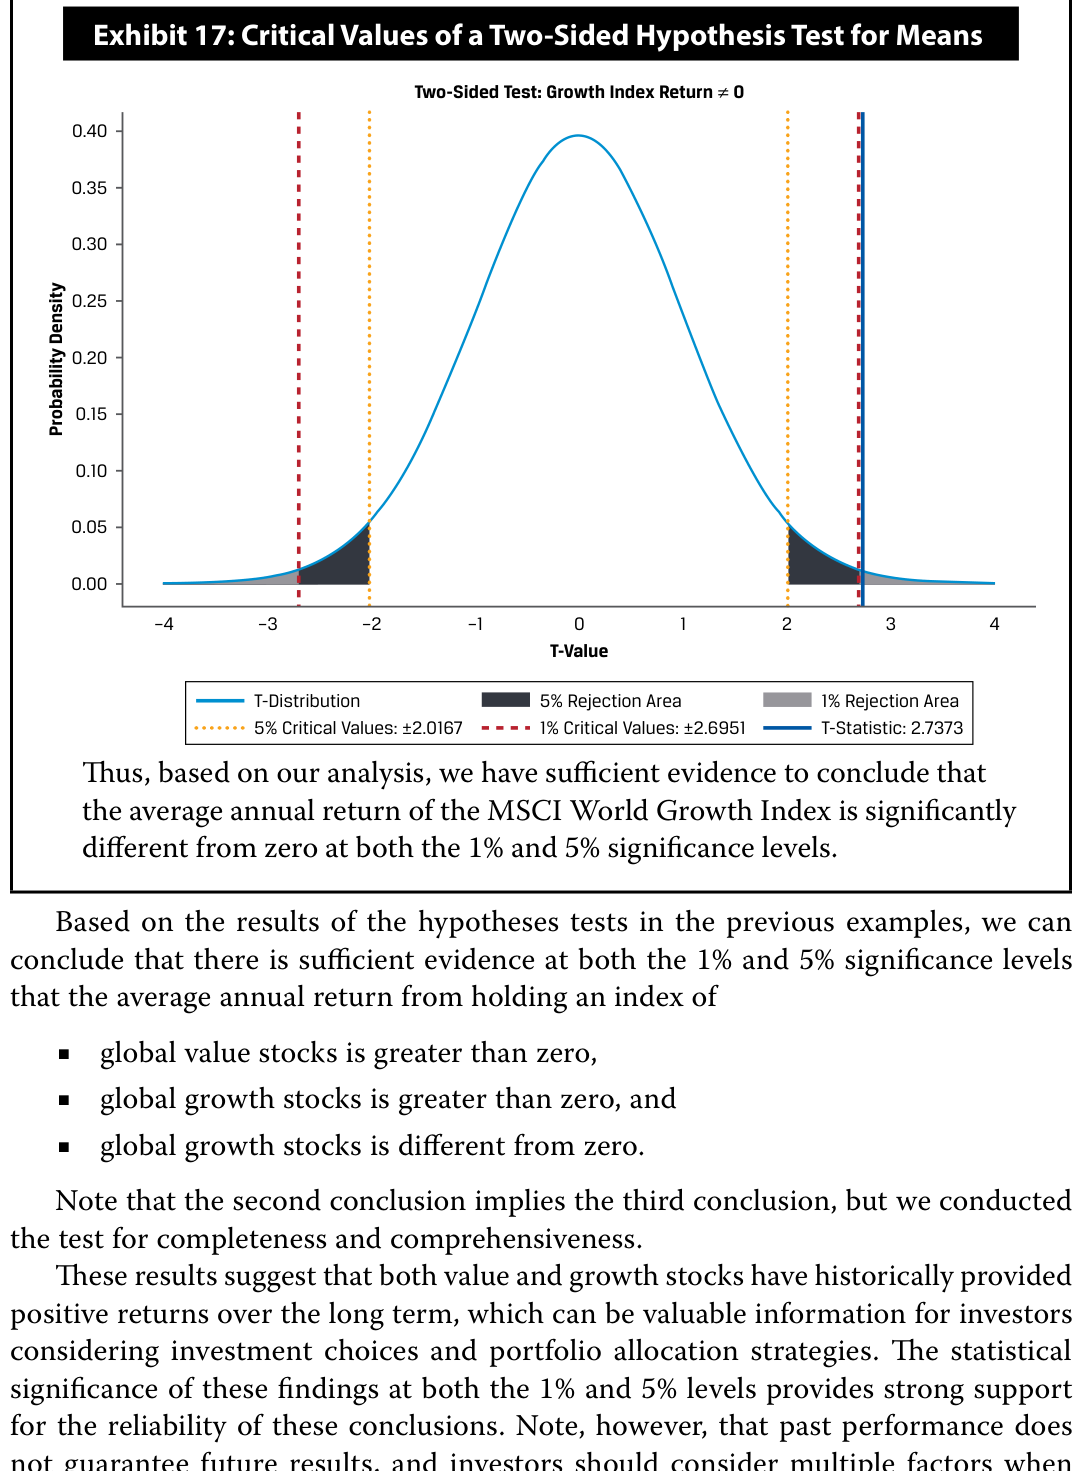
\includegraphics[width=0.75\linewidth]{002_figs/007_Module_7/exhibit_17.png}
	\caption{Two-Sided Mean Test Critical Values and Rejection Regions}
	\label{fig:mod7_exhibit_17}
\end{figure}
% Reference: CFA Curriculum 2027, Volume 1, Module 7, Page 350, Exhibit 17

\subsubsection{Test of a Single Variance}
To test the variance of a single normally distributed population, we use the Chi-square ($\chi^2$) test statistic with $n - 1$ degrees of freedom (Exhibit~\ref{fig:mod7_exhibit_18}):
\begin{equation}
	\chi^2 = \frac{(n-1)s^2}{\sigma_0^2}
	\label{eq:single_variance_chisq_m7}
\end{equation}
% Reference: CFA Curriculum 2027, Volume 1, Module 7, Page 351, Equation (7)

\begin{figure}[!htbp]
	\centering
	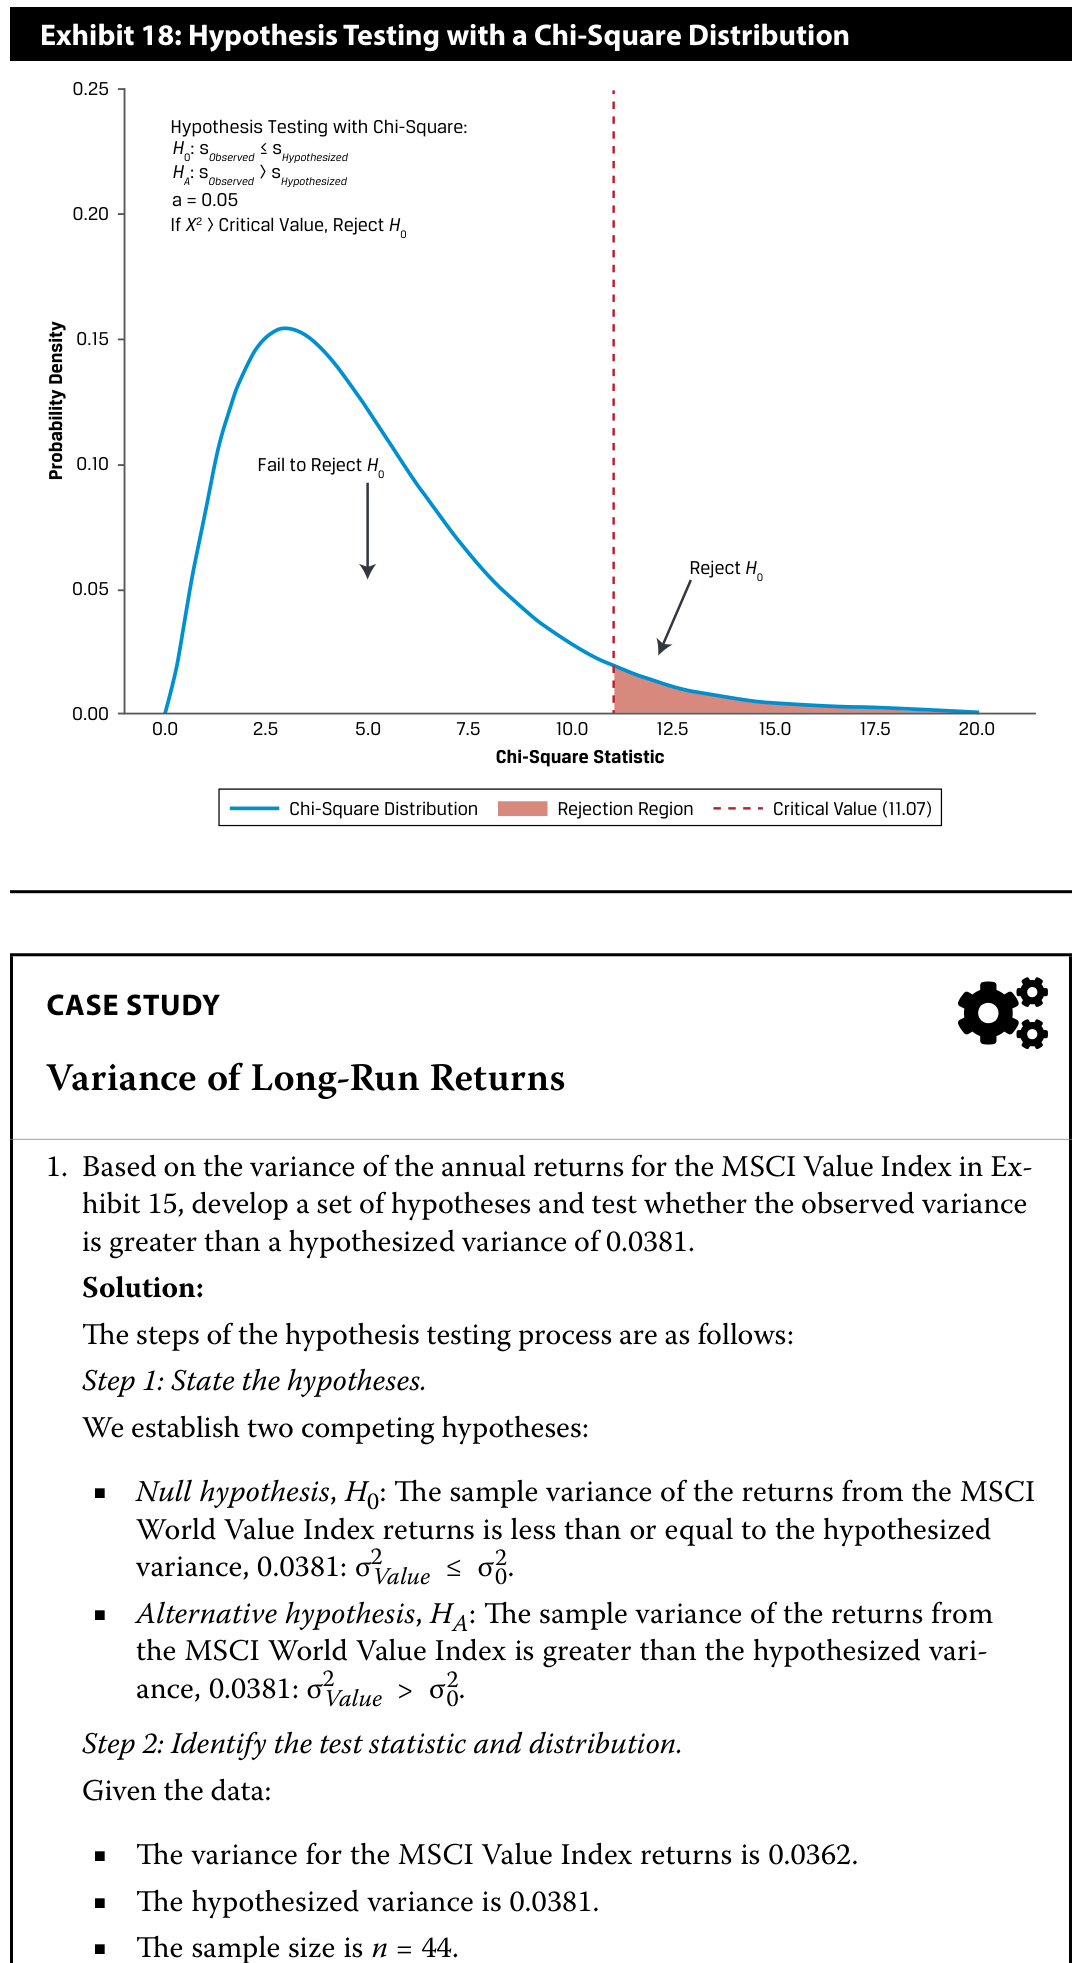
\includegraphics[width=0.75\linewidth]{002_figs/007_Module_7/exhibit_18.png}
	\caption{Hypothesis Testing with a Chi-Square Distribution ($df=5$)}
	\label{fig:mod7_exhibit_18}
\end{figure}
% Reference: CFA Curriculum 2027, Volume 1, Module 7, Page 352, Exhibit 18

\begin{tcolorbox}[
	colback=gray!5!white,
	colframe=black!15!white,
	boxrule=0.5pt,
	arc=3pt,
	title=\textbf{Case Study: Testing MSCI Value Index Variance},
	coltitle=black,
	colbacktitle=black!5!white,
	before skip=6pt,
	after skip=6pt,
	breakable
]
We test whether the variance of the Value Index is greater than $0.0381$ ($H_0: \sigma^2 \le 0.0381$ vs $H_A: \sigma^2 > 0.0381$).
\begin{enumerate}
	\item \textbf{Calculate Test Statistic ($df = 43$):} $\chi^2 = \frac{43 \times 0.0362}{0.0381} \approx 40.8237$.
	\item \textbf{Decision Rule:} Right-tailed critical values are $\chi^2_{0.05} = 59.3035$ and $\chi^2_{0.01} = 67.4593$ (Exhibit~\ref{fig:mod7_exhibit_19}).
	\item \textbf{Conclusion:} Since $40.8237 < 59.3035$, we fail to reject $H_0$. The variance is not significantly greater than $0.0381$.
\end{enumerate}
\end{tcolorbox}

\begin{figure}[!htbp]
	\centering
	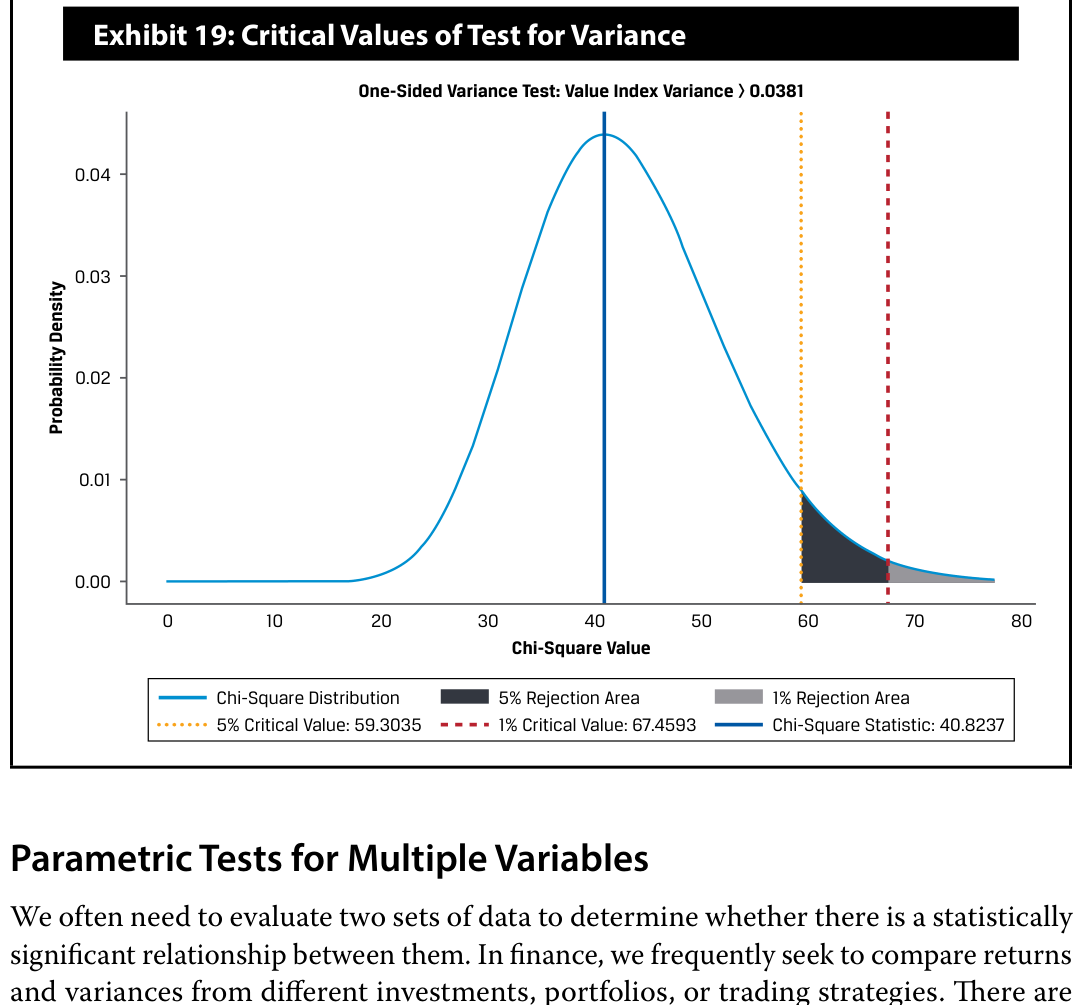
\includegraphics[width=0.75\linewidth]{002_figs/007_Module_7/exhibit_19.png}
	\caption{One-Sided Variance Test Critical Values and Rejection Regions}
	\label{fig:mod7_exhibit_19}
\end{figure}
% Reference: CFA Curriculum 2027, Volume 1, Module 7, Page 353, Exhibit 19

\subsection{Parametric Tests for Multiple Variables}
We compare the means and variances of two populations.

\subsubsection{Test of Equality of Two Unknown Means (Independent Samples)}
Assuming equal population variances, the $t$-test statistic with $n_1 + n_2 - 2$ degrees of freedom is:
\begin{equation}
	t = \frac{(\bar{X}_1 - \bar{X}_2) - \Delta_0}{\sqrt{\frac{s_p^2}{n_1} + \frac{s_p^2}{n_2}}} \quad \text{where} \quad s_p^2 = \frac{(n_1-1)s_1^2 + (n_2-1)s_2^2}{n_1+n_2-2}
	\label{eq:indep_means_t_test_m7}
\end{equation}
% Reference: CFA Curriculum 2027, Volume 1, Module 7, Page 354, Equation (8)

\begin{tcolorbox}[
	colback=gray!5!white,
	colframe=black!15!white,
	boxrule=0.5pt,
	arc=3pt,
	title=\textbf{Case Study: Comparing Growth vs Value Average Returns},
	coltitle=black,
	colbacktitle=black!5!white,
	before skip=6pt,
	after skip=6pt,
	breakable
]
We test whether Growth average returns exceed Value returns ($H_0: \mu_G - \mu_V \le 0$ vs $H_A: \mu_G - \mu_V > 0$).
\begin{enumerate}
	\item \textbf{Calculate Test Statistic ($df = 86$):}
	      \[ t = \frac{0.0881 - 0.0717 - 0}{\sqrt{\frac{0.0456}{44} + \frac{0.0362}{44}}} = \frac{0.0164}{0.0431} \approx 0.3805 \]
	\item \textbf{Decision Rule:} One-tailed critical values are $t_{0.05} = 1.6628$ and $t_{0.01} = 2.3705$ (Exhibit~\ref{fig:mod7_exhibit_20}).
	\item \textbf{Conclusion:} Since $0.3805 < 1.6628$, we fail to reject $H_0$. The difference in average returns is not statistically significant.
\end{enumerate}
\end{tcolorbox}

\begin{figure}[!htbp]
	\centering
	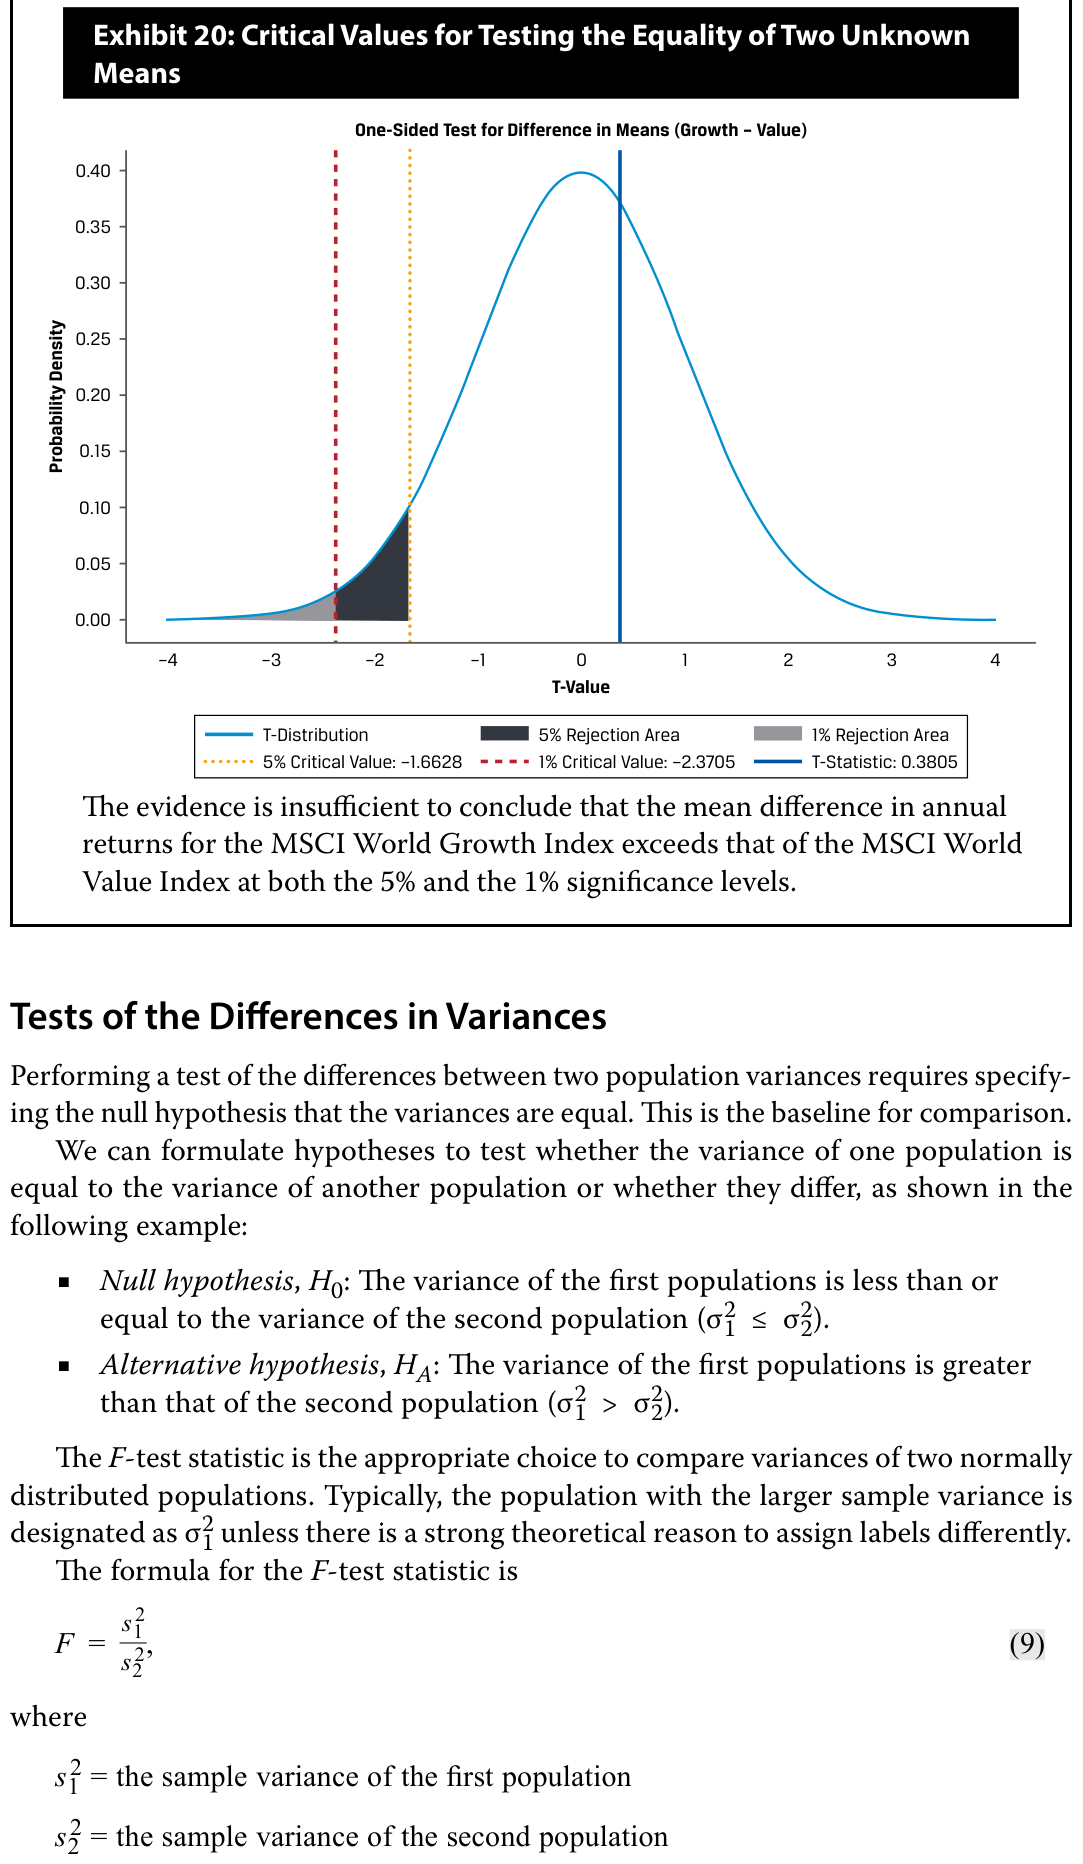
\includegraphics[width=0.75\linewidth]{002_figs/007_Module_7/exhibit_20.png}
	\caption{Independent Means Test Critical Values and Rejection Regions}
	\label{fig:mod7_exhibit_20}
\end{figure}
% Reference: CFA Curriculum 2027, Volume 1, Module 7, Page 356, Exhibit 20

\subsubsection{Test of Difference in Two Variances ($F$-test)}
To compare variances of two independent, normally distributed populations, the $F$-test statistic is:
\begin{equation}
	F = \frac{s_1^2}{s_2^2} \quad (\text{where } s_1^2 \ge s_2^2)
	\label{eq:variance_ratio_f_test_m7}
\end{equation}
% Reference: CFA Curriculum 2027, Volume 1, Module 7, Page 356, Equation (9)
With $df_1 = n_1 - 1$ and $df_2 = n_2 - 1$ (Exhibit~\ref{fig:mod7_exhibit_21}).

\begin{figure}[!htbp]
	\centering
	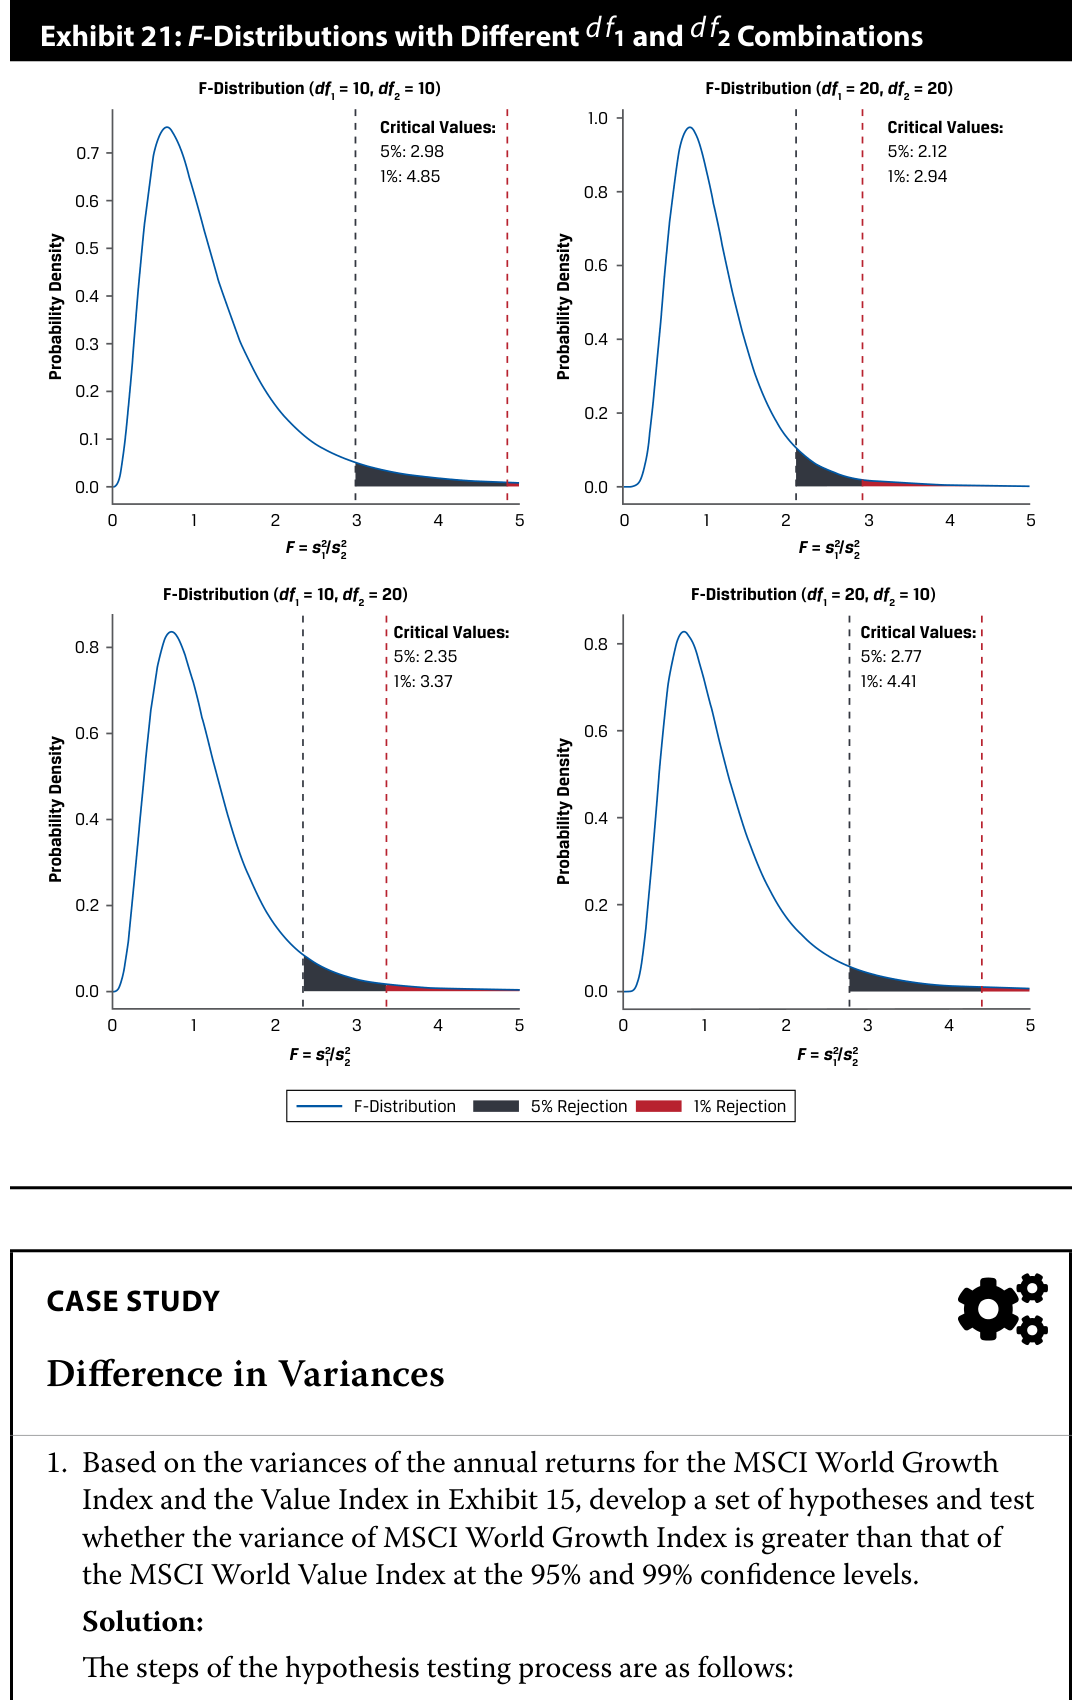
\includegraphics[width=0.85\linewidth]{002_figs/007_Module_7/exhibit_21.png}
	\caption{$F$-Distributions with Different Degrees of Freedom}
	\label{fig:mod7_exhibit_21}
\end{figure}
% Reference: CFA Curriculum 2027, Volume 1, Module 7, Page 357, Exhibit 21

\begin{tcolorbox}[
	colback=gray!5!white,
	colframe=black!15!white,
	boxrule=0.5pt,
	arc=3pt,
	title=\textbf{Case Study: Comparing Growth vs Value Variances},
	coltitle=black,
	colbacktitle=black!5!white,
	before skip=6pt,
	after skip=6pt,
	breakable
]
We test whether Growth variance is greater than Value variance ($H_0: \sigma_G^2 \le \sigma_V^2$ vs $H_A: \sigma_G^2 > \sigma_V^2$).
\begin{enumerate}
	\item \textbf{Calculate Test Statistic ($df_1 = 43, df_2 = 43$):} $F = \frac{0.0456}{0.0362} \approx 1.2595$.
	\item \textbf{Decision Rule:} Critical values are $F_{0.05} = 1.6607$ and $F_{0.01} = 2.0569$ (Exhibit~\ref{fig:mod7_exhibit_22}).
	\item \textbf{Conclusion:} Since $1.2595 < 1.6607$, we fail to reject $H_0$. Growth variance is not significantly larger.
\end{enumerate}
\end{tcolorbox}


\begin{figure}[!htbp]
	\centering
	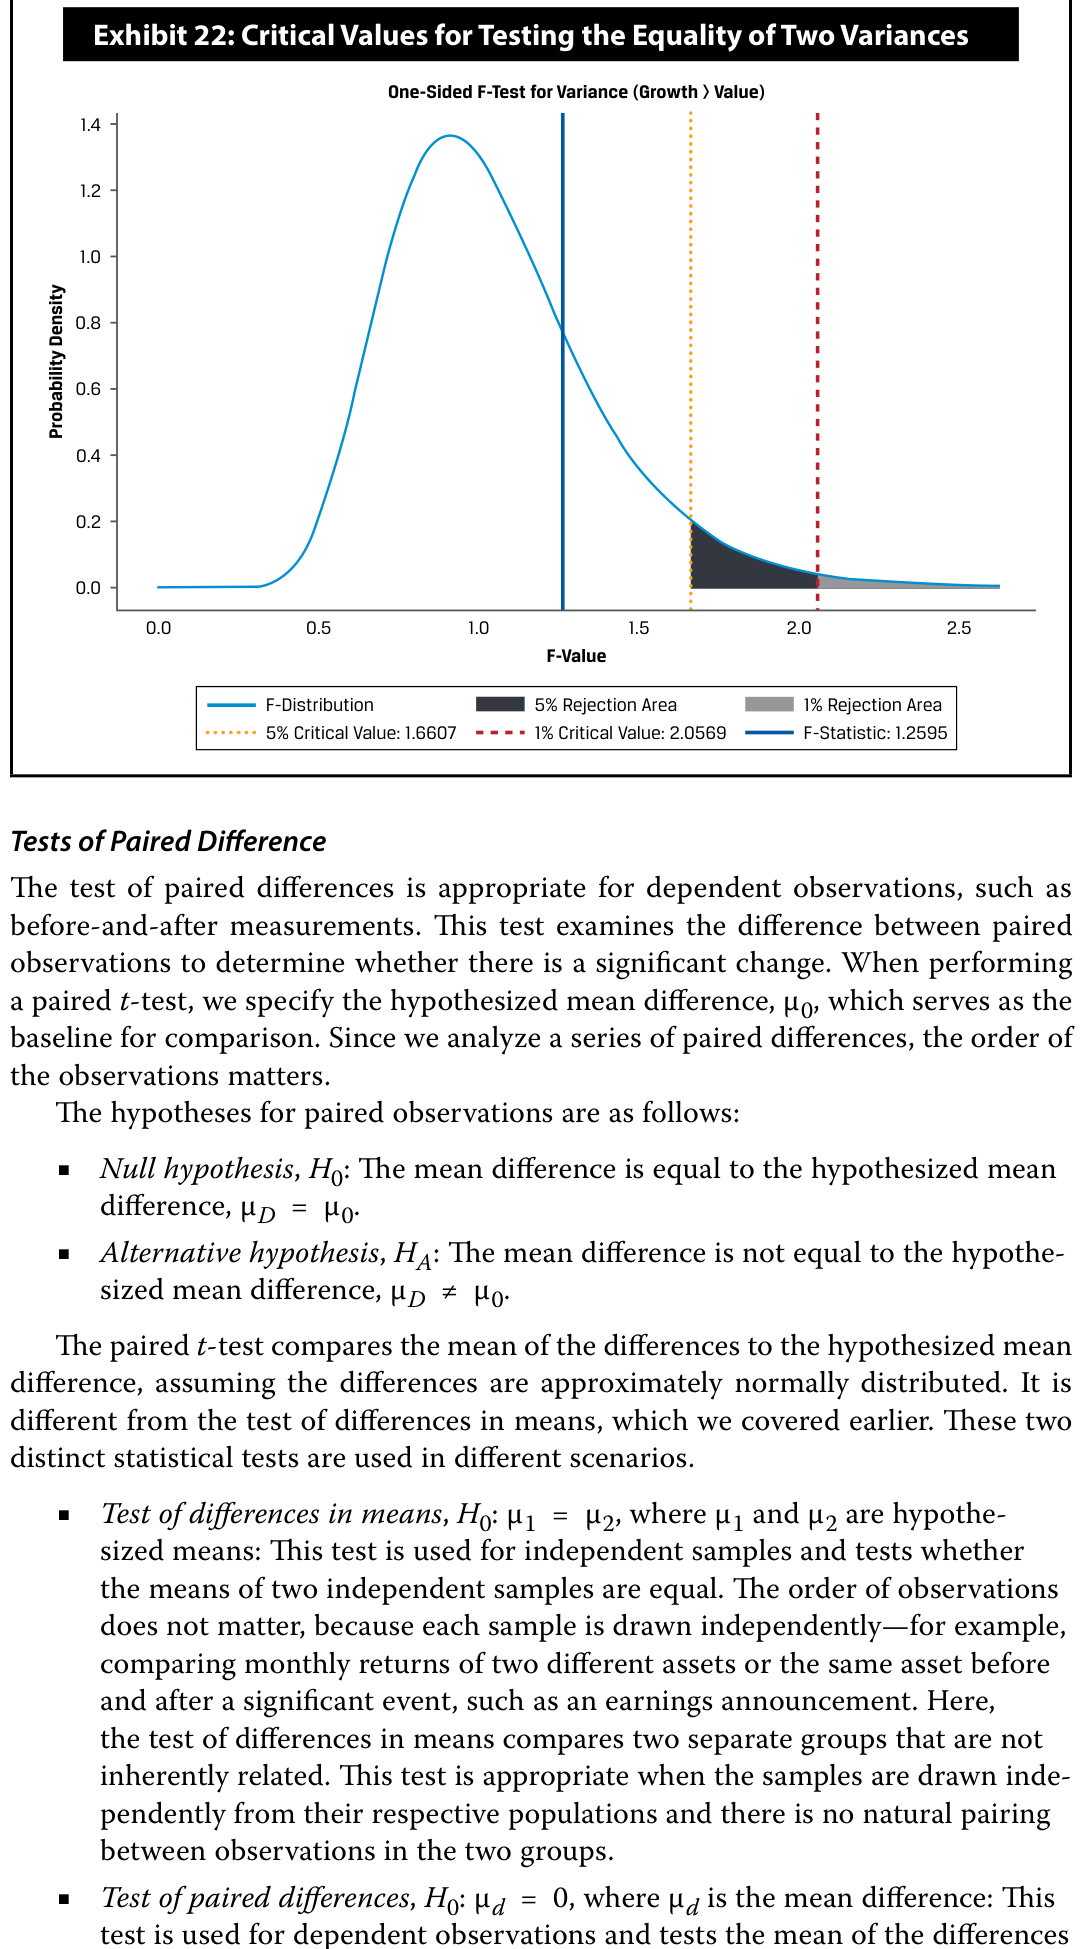
\includegraphics[width=0.75\linewidth]{002_figs/007_Module_7/exhibit_22.png}
	\caption{Equality of Variances $F$-Test Critical Values}
	\label{fig:mod7_exhibit_22}
\end{figure}
% Reference: CFA Curriculum 2027, Volume 1, Module 7, Page 359, Exhibit 22

\subsubsection{Test of Paired Differences (Dependent Samples)}
For dependent observations, the $t$-test statistic with $n - 1$ degrees of freedom is:
\begin{equation}
	t = \frac{\bar{d} - \mu_{d0}}{s_d / \sqrt{n}}
	\label{eq:paired_means_t_test_m7}
\end{equation}
% Reference: CFA Curriculum 2027, Volume 1, Module 7, Page 360, Equation (10)
Where $\bar{d}$ is the sample mean difference, and $s_d$ is the sample standard deviation of differences.

\begin{tcolorbox}[
	colback=gray!5!white,
	colframe=black!15!white,
	boxrule=0.5pt,
	arc=3pt,
	title=\textbf{Case Study: Paired Difference of Growth and Value Returns},
	coltitle=black,
	colbacktitle=black!5!white,
	before skip=6pt,
	after skip=6pt,
	breakable
]
We test whether the mean difference in paired returns is different from zero ($H_0: \mu_d = 0$ vs $H_A: \mu_d \ne 0$). We calculate $\bar{d} = 1.64\%$ and $s_d = 10.62\%$.
\begin{enumerate}
	\item \textbf{Calculate Test Statistic ($df = 43$):} $t = \frac{0.0164 - 0}{0.1062 / \sqrt{44}} \approx 1.0243$.
	\item \textbf{Decision Rule:} Two-tailed critical values are $\pm 2.0167$ (at 5\% significance, Exhibit~\ref{fig:mod7_exhibit_23}).
	\item \textbf{Conclusion:} Since $1.0243 < 2.0167$, we fail to reject $H_0$. The paired differences are not statistically significant.
\end{enumerate}
\end{tcolorbox}

\begin{figure}[!htbp]
	\centering
	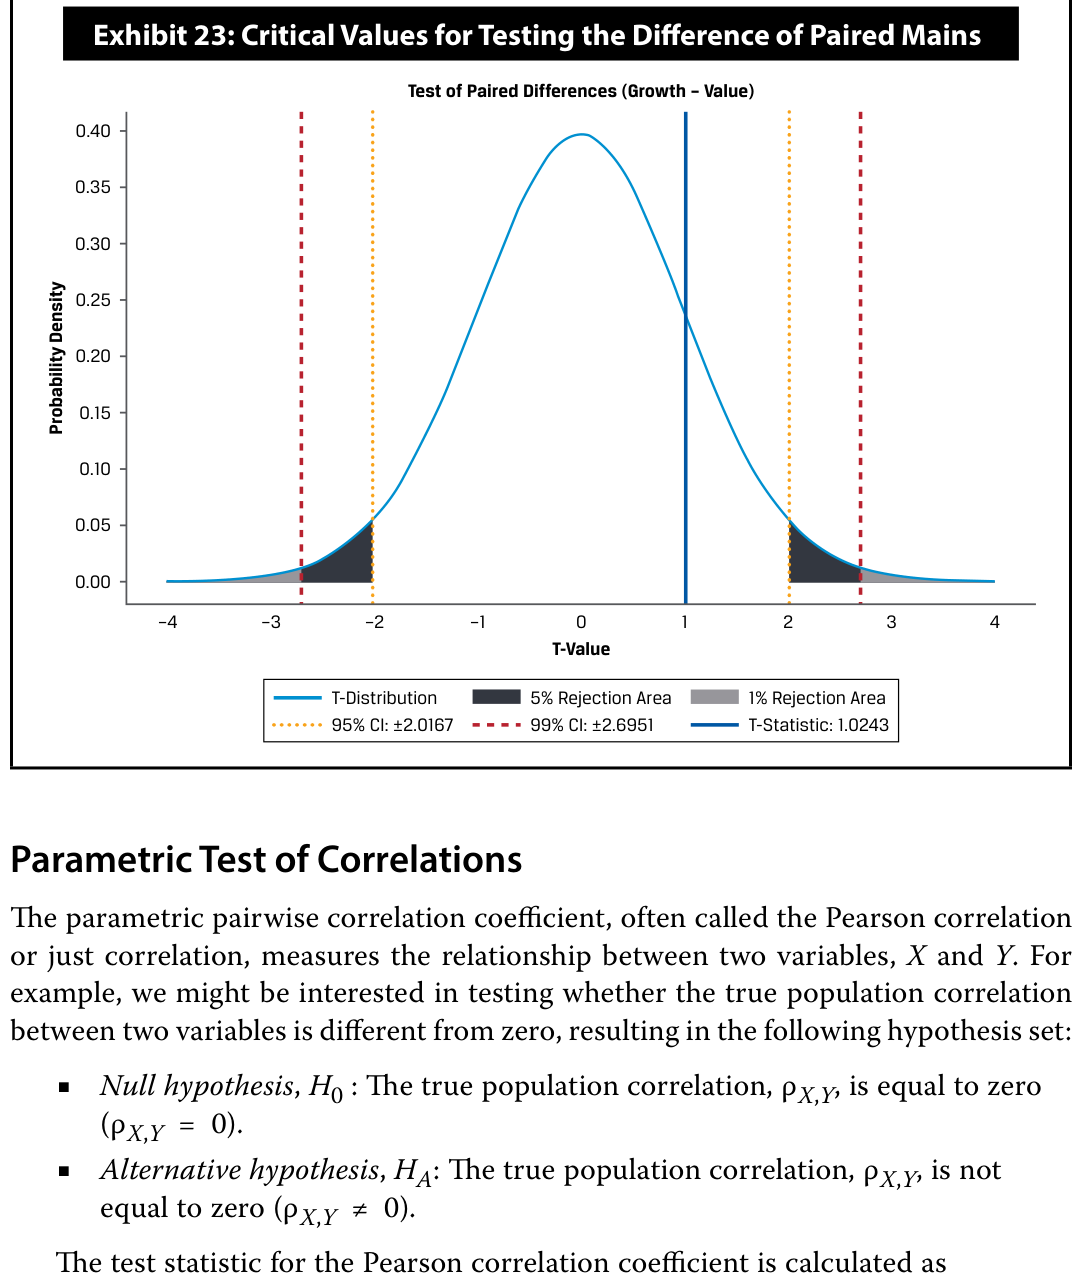
\includegraphics[width=0.75\linewidth]{002_figs/007_Module_7/exhibit_23.png}
	\caption{Paired Means Test Critical Values and Rejection Regions}
	\label{fig:mod7_exhibit_23}
\end{figure}
% Reference: CFA Curriculum 2027, Volume 1, Module 7, Page 361, Exhibit 23

\subsubsection{Parametric Test of Correlations}
To test whether the Pearson correlation coefficient between $X$ and $Y$ is zero ($H_0: \rho = 0$ vs $H_A: \rho \ne 0$), we use the $t$-test statistic with $n - 2$ degrees of freedom:
\begin{equation}
	t = \frac{r \sqrt{n-2}}{\sqrt{1 - r^2}}
	\label{eq:correlation_t_test_m7}
\end{equation}
% Reference: CFA Curriculum 2027, Volume 1, Module 7, Page 361, Equation (11)

As sample size $n$ increases, the standard error decreases, causing the power of the test to increase. Thus, in very large datasets, even minor correlations are rejected as statistically different from zero (Exhibit~\ref{fig:mod7_exhibit_24}).

\begin{figure}[!htbp]
	\centering
	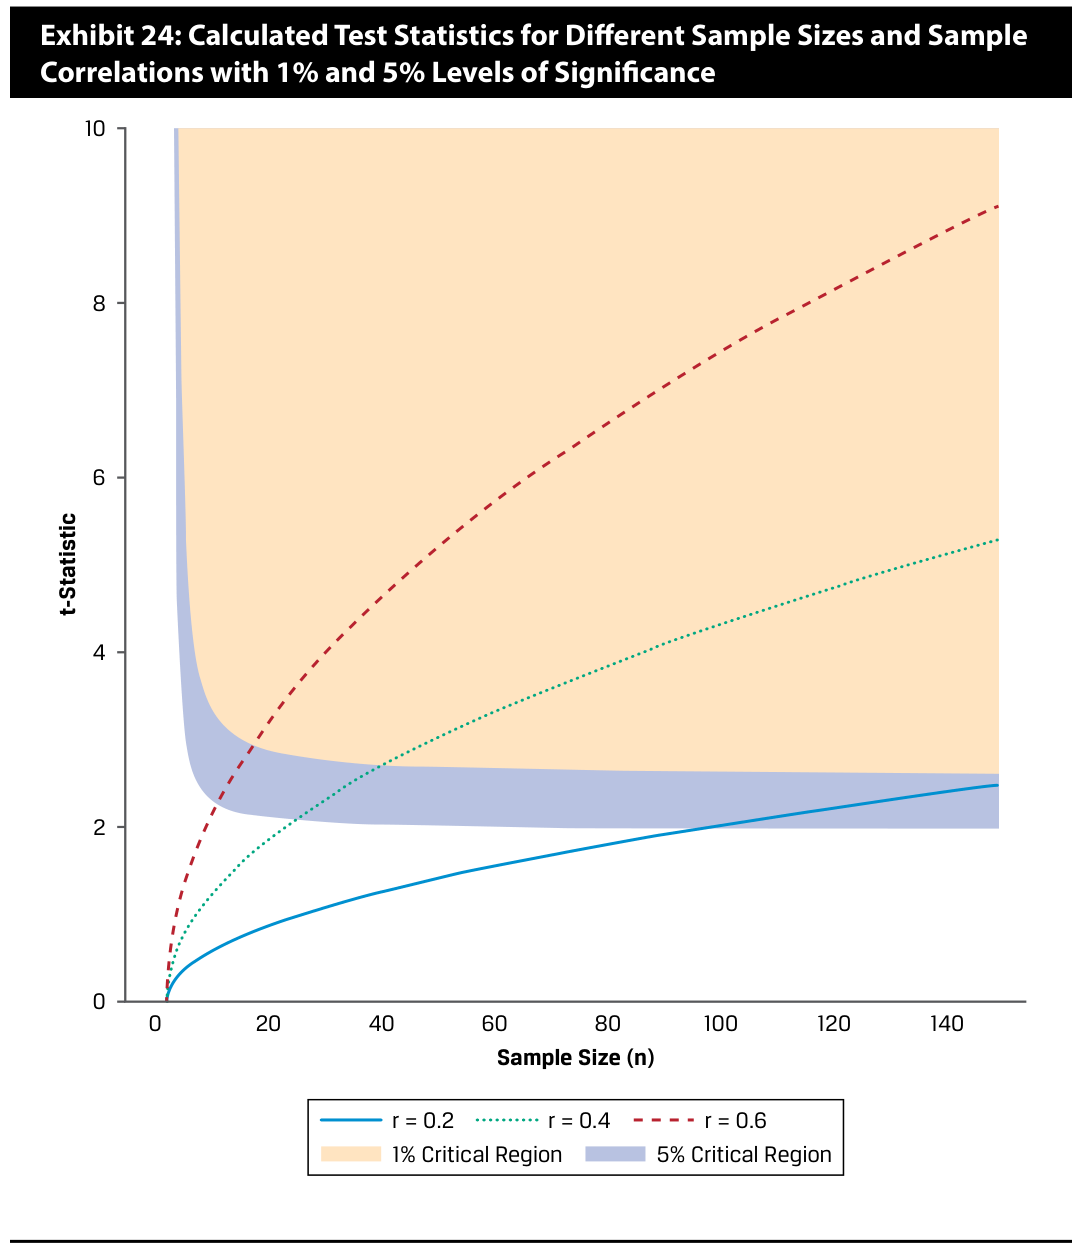
\includegraphics[width=0.75\linewidth]{002_figs/007_Module_7/exhibit_24.png}
	\caption{t-Statistic Values for Various Sample Sizes and Correlation Coefficients}
	\label{fig:mod7_exhibit_24}
\end{figure}
% Reference: CFA Curriculum 2027, Volume 1, Module 7, Page 362, Exhibit 24

\begin{tcolorbox}[
	colback=gray!5!white,
	colframe=black!15!white,
	boxrule=0.5pt,
	arc=3pt,
	title=\textbf{Case Study: Fund Correlations and STOXX50 Index},
	coltitle=black,
	colbacktitle=black!5!white,
	before skip=6pt,
	after skip=6pt,
	breakable
]
Table~\ref{tab:fund_correlations_m7} presents correlations of four funds with the STOXX50 index ($n = 36$, $df = 34$). The critical t-value at the 5\% significance level is $\pm 2.032$.
For Fund 3 and Fund 4:
\[ t = \frac{0.3102\sqrt{34}}{\sqrt{1 - 0.3102^2}} \approx 1.903 \]
Since $1.903 < 2.032$, the correlation between Fund 3 and Fund 4 is not statistically significant. However, all other correlations (e.g., Fund 2 and STOXX50, $r=0.8223 \implies t=8.426$) are statistically significant, suggesting limited diversification benefits except between Fund 3 and 4.
\end{tcolorbox}

\begin{table}[!htbp]
\centering
\caption{Fund Correlations Matrix ($n=36$)}
\label{tab:fund_correlations_m7}
\begin{tabular}{p{0.15\linewidth} p{0.14\linewidth} p{0.14\linewidth} p{0.14\linewidth} p{0.14\linewidth} p{0.14\linewidth}}
\toprule
\textbf{Asset} & \textbf{Fund 1} & \textbf{Fund 2} & \textbf{Fund 3} & \textbf{Fund 4} & \textbf{STOXX50} \\
\midrule
\textbf{Fund 1} & 1.0000 & --- & --- & --- & --- \\
\textbf{Fund 2} & 0.9231 & 1.0000 & --- & --- & --- \\
\textbf{Fund 3} & 0.4771 & 0.4156 & 1.0000 & --- & --- \\
\textbf{Fund 4} & 0.7111 & 0.7238 & 0.3102 & 1.0000 & --- \\
\textbf{STOXX50} & 0.8277 & 0.8223 & 0.5791 & 0.7515 & 1.0000 \\
\bottomrule
\end{tabular}
\end{table}
% Reference: CFA Curriculum 2027, Volume 1, Module 7, Page 363

\subsection{P-Value and P-Hacking}
The p-value is the smallest level of significance at which we reject the null hypothesis:
\begin{itemize}
	\item \textbf{Decision Rule:} Reject $H_0$ if $p\text{-value} < \alpha$; otherwise, fail to reject.
\end{itemize}
For the MSCI Value Index mean test ($t = 2.5001$, $df = 43$), the one-tailed $p$-value is $0.0081$, which is less than both $5\%$ and $1\%$, leading to rejection of $H_0$.

\begin{examtip}
\textbf{Beware of P-Hacking}\\
p-hacking refers to the practice of manipulating data or models (such as trimming time horizons, selectively removing outliers, or testing dozens of models) until a statistically significant result ($p < 0.05$) is obtained. This inflates the Type I error rate. To prevent p-hacking, analysts must use out-of-sample validation and strict methodologies.
\end{examtip}

\subsection{Practical Implementation (Excel and Google Sheets)}
Table~\ref{tab:excel_functions_m7} lists functions to compute critical values for hypothesis testing.

\begin{table}[!htbp]
\centering
\caption{Built-In Excel and Google Sheet Functions for Hypothesis Testing}
\label{tab:excel_functions_m7}
\begin{tabular}{p{0.22\linewidth} | p{0.34\linewidth} | p{0.34\linewidth}}
\toprule
\textbf{Function} & \textbf{Excel Formula} & \textbf{Google Sheets Formula} \\
\midrule
Inverse Student's t & \texttt{=T.INV(prob, df)} & \texttt{=T.INV(prob, df)} \\
Two-tailed t Inverse & \texttt{=T.INV.2T(prob, df)} & \texttt{=T.INV.2T(prob, df)} \\
Right-tailed t Dist & \texttt{=T.DIST.RT(x, df)} & \texttt{=T.DIST.RT(x, df)} \\
Inverse Standard Normal & \texttt{=NORM.S.INV(prob)} & \texttt{=NORM.S.INV(prob)} \\
Inverse Normal Cumulative & \texttt{=NORM.INV(prob, mean, sd)} & \texttt{=NORM.INV(prob, mean, sd)} \\
Inverse Chi-Square & \texttt{=CHISQ.INV.RT(prob, df)} & \texttt{=CHISQ.INV.RT(prob, df)} \\
Inverse Left-tail F & \texttt{=F.INV(prob, df1, df2)} & \texttt{=F.INV(prob, df1, df2)} \\
Inverse Right-tail F & \texttt{=F.INV.RT(prob, df1, df2)} & \texttt{=F.INV.RT(prob, df1, df2)} \\
\bottomrule
\end{tabular}
\end{table}
% Reference: CFA Curriculum 2027, Volume 1, Module 7, Page 366, Exhibit 25

\section{NON-PARAMETRIC TESTS}
\begin{center}
\begin{tabular}{p{0.06\linewidth} | p{0.88\linewidth}}
	c & compare and contrast parametric and non-parametric tests, describe situations in which each is the more appropriate type of test, construct appropriate hypothesis tests, and interpret the results \\
\end{tabular}
\end{center}

\textcolor{blue}{\textit{Thực tế: Khi dữ liệu không chuẩn (đuôi béo, lệch) hoặc ở dạng định danh/thứ bậc, kiểm định phi tham số (Non-parametric) như Spearman hoặc Chi-square test of independence là bắt buộc để tránh kết luận sai lệch.}}

\subsection{Comparison of Parametric and Non-Parametric Tests}
\begin{itemize}
	\item \textbf{Parametric Tests:} Perform testing using parameters (mean, variance) and require specific distribution assumptions (e.g., normality). They are more powerful if assumptions are met.
	\item \textbf{Non-Parametric Tests:} Do not make distribution assumptions. They are suitable for ordinal/categorical data, small sample sizes, or when outliers skew parametric estimations. However, they are less powerful when normality assumptions hold.
\end{itemize}

\subsection{Non-Parametric Test for Correlation (Spearman Rank Correlation)}
The Spearman rank correlation coefficient ($r_s$) evaluates monotonic (not necessarily linear) relationships by analyzing the ranks of variables:
\begin{equation}
	r_s = 1 - \frac{6 \sum_{i=1}^n d_i^2}{n(n^2 - 1)}
	\label{eq:spearman_formula_m7}
\end{equation}
% Reference: CFA Curriculum 2027, Volume 1, Module 7, Page 370
Where $d_i$ is the difference in ranks for each observation pair. For $n > 30$, the test statistic follows a $t$-distribution with $n - 2$ degrees of freedom:
\begin{equation}
	t = \frac{r_s \sqrt{n-2}}{\sqrt{1 - r_s^2}}
	\label{eq:spearman_t_test_m7}
\end{equation}
% Reference: CFA Curriculum 2027, Volume 1, Volume 7, Page 370, Equation (12)

\begin{tcolorbox}[
	colback=gray!5!white,
	colframe=black!15!white,
	boxrule=0.5pt,
	arc=3pt,
	title=\textbf{Case Study: Is Gold an Inflation Hedge?},
	coltitle=black,
	colbacktitle=black!5!white,
	before skip=6pt,
	after skip=6pt,
	breakable
]
Using 24 years of monthly observations ($n = 288$), we analyze German inflation and gold price returns in EUR (Exhibit~\ref{fig:mod7_exhibit_26} \& Exhibit~\ref{fig:mod7_exhibit_28}). Inflation is highly skewed ($2.2507$) and leptokurtic ($5.8089$), violating normality.
\begin{itemize}
	\item \textbf{Pearson Correlation:} $r = -0.0086 \implies t = -0.1454$. Critical value at 5\% is $\pm 1.96$. Not statistically significant.
	\item \textbf{Spearman Rank Correlation:} $r_s = 0.0480 \implies t = \frac{0.0480\sqrt{286}}{\sqrt{1-0.0480^2}} \approx 0.8127$.
\end{itemize}
Since $0.8127 < 1.96$, we fail to reject the null hypothesis of no monotonic correlation. There is insufficient evidence that gold is a good inflation hedge in Germany.
\end{tcolorbox}

\begin{figure}[!htbp]
	\centering
	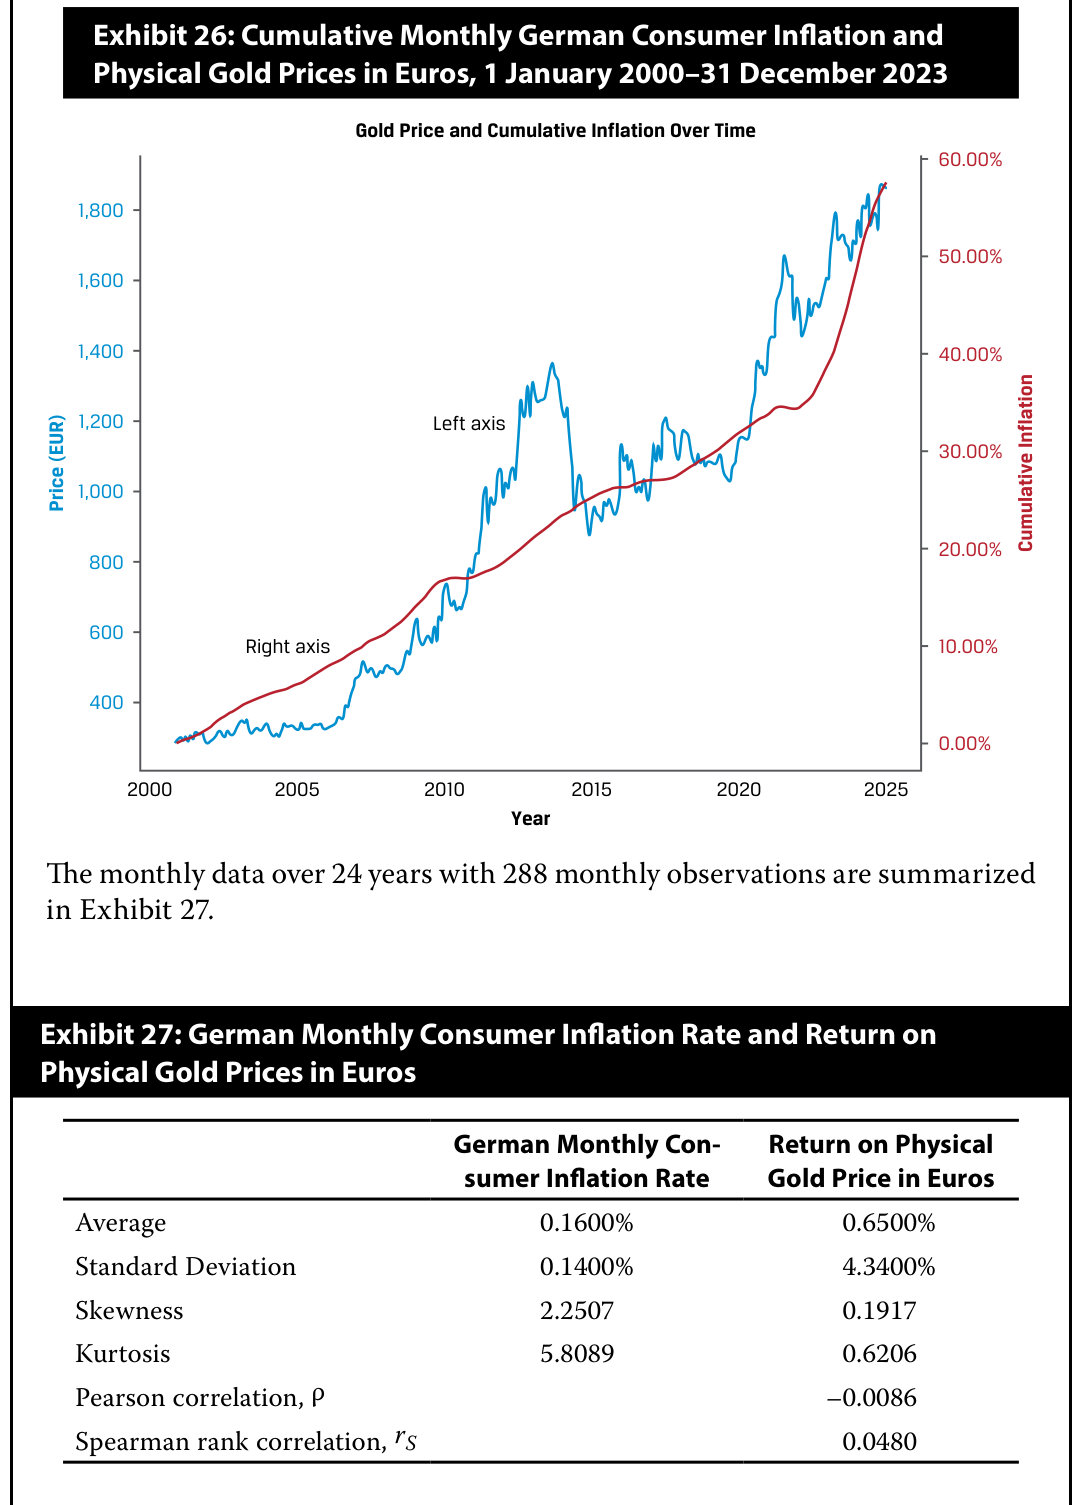
\includegraphics[width=0.75\linewidth]{002_figs/007_Module_7/exhibit_26.png}
	\caption{German Consumer Inflation and Physical Gold Prices (EUR)}
	\label{fig:mod7_exhibit_26}
\end{figure}
% Reference: CFA Curriculum 2027, Volume 1, Module 7, Page 371, Exhibit 26

\begin{figure}[!htbp]
	\centering
	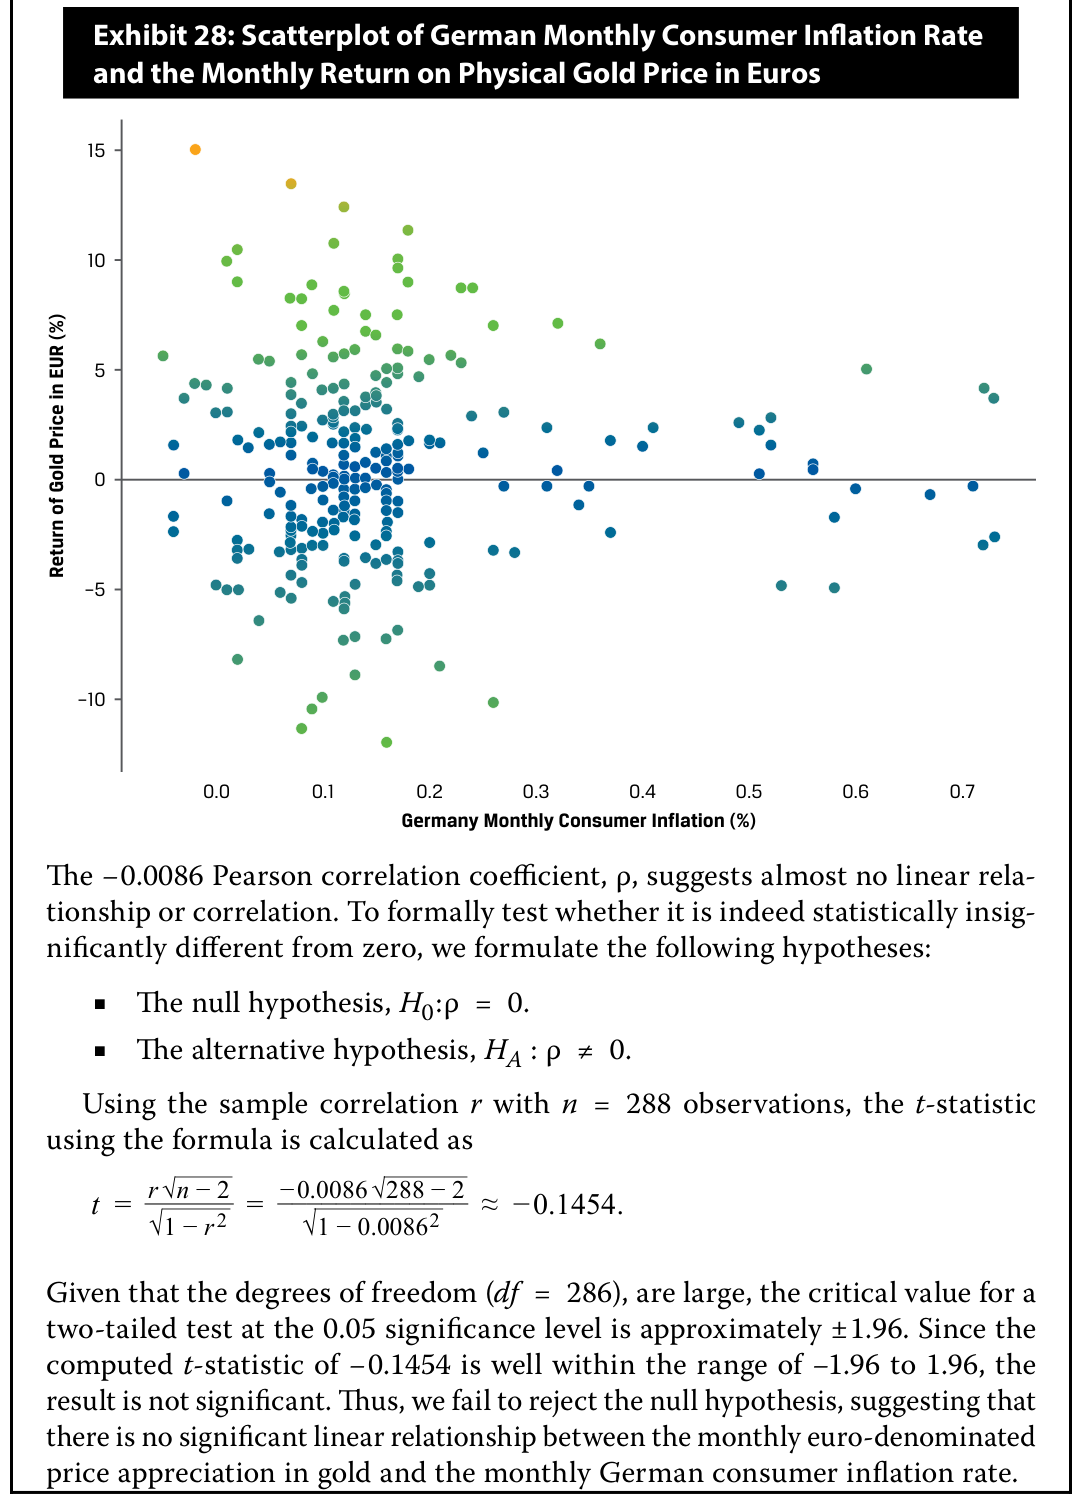
\includegraphics[width=0.75\linewidth]{002_figs/007_Module_7/exhibit_28.png}
	\caption{Scatterplot of German Inflation and Gold returns}
	\label{fig:mod7_exhibit_28}
\end{figure}
% Reference: CFA Curriculum 2027, Volume 1, Module 7, Page 372, Exhibit 28

\subsection{Chi-Square Test of Independence}
For categorical data, we test whether classifications are independent using a Chi-square test statistic with $df = (r - 1)(c - 1)$:
\begin{equation}
	\chi^2 = \sum_{i=1}^r \sum_{j=1}^c \frac{(O_{ij} - E_{ij})^2}{E_{ij}}
	\label{eq:chisq_independence_m7}
\end{equation}
% Reference: CFA Curriculum 2027, Volume 1, Module 7, Page 375, Equation (14)

Where $O_{ij}$ is the observed frequency and $E_{ij}$ is the expected frequency assuming independence:
\begin{equation}
	E_{ij} = \frac{(\text{Total Row } i) \times (\text{Total Column } j)}{\text{Overall Total } N}
	\label{eq:expected_freq_m7}
\end{equation}
% Reference: CFA Curriculum 2027, Volume 1, Module 7, Page 374, Equation (13)

Standardized residuals help identify which cells deviate significantly (values exceeding $\pm 1.96$ are significant):
\begin{equation}
	\text{Standardized Residual} = \frac{O_{ij} - E_{ij}}{\sqrt{E_{ij}}}
	\label{eq:standardized_residual_m7}
\end{equation}
% Reference: CFA Curriculum 2027, Volume 1, Module 7, Page 377, Equation (15)

\begin{tcolorbox}[
	colback=gray!5!white,
	colframe=black!15!white,
	boxrule=0.5pt,
	arc=3pt,
	title=\textbf{Case Study: Comparing Environmental and Governance Ratings},
	coltitle=black,
	colbacktitle=black!5!white,
	before skip=6pt,
	after skip=6pt,
	breakable
]
We examine the independence of ESG ratings of 500 firms (Table~\ref{tab:esg_contingency_m7}). Expected frequency $E_{22}$ (Average/Average) is $\frac{260 \times 230}{500} = 119.6$. Summing scaled squared deviations (Exhibit~\ref{fig:mod7_exhibit_31}), we obtain $\chi^2 \approx 35.75$. With $df = (3-1)(3-1) = 4$, the critical value at 5\% is $\chi^2_{0.05} = 9.49$. Since $35.75 > 9.49$, we reject the null hypothesis of independence. Environmental and governance ratings are related.
\end{tcolorbox}

\begin{table}[!htbp]
\centering
\caption{ESG Ratings Contingency Table ($N=500$)}
\label{tab:esg_contingency_m7}
\begin{tabular}{p{0.35\linewidth} p{0.15\linewidth} p{0.13\linewidth} p{0.12\linewidth} p{0.10\linewidth}}
\toprule
\textbf{Environmental Rating} & \textbf{Progressive (GR1)} & \textbf{Average (GR2)} & \textbf{Poor (GR3)} & \textbf{Total} \\
\midrule
\textbf{Progressive (ER1)} & 35 & 40 & 5 & 80 \\
\textbf{Average (ER2)} & 80 & 130 & 50 & 260 \\
\textbf{Poor (ER3)} & 40 & 60 & 60 & 160 \\
\midrule
\textbf{Total} & 155 & 230 & 115 & 500 \\
\bottomrule
\end{tabular}
\end{table}
% Reference: CFA Curriculum 2027, Volume 1, Module 7, Page 373, Exhibit 29

\begin{figure}[!htbp]
	\centering
	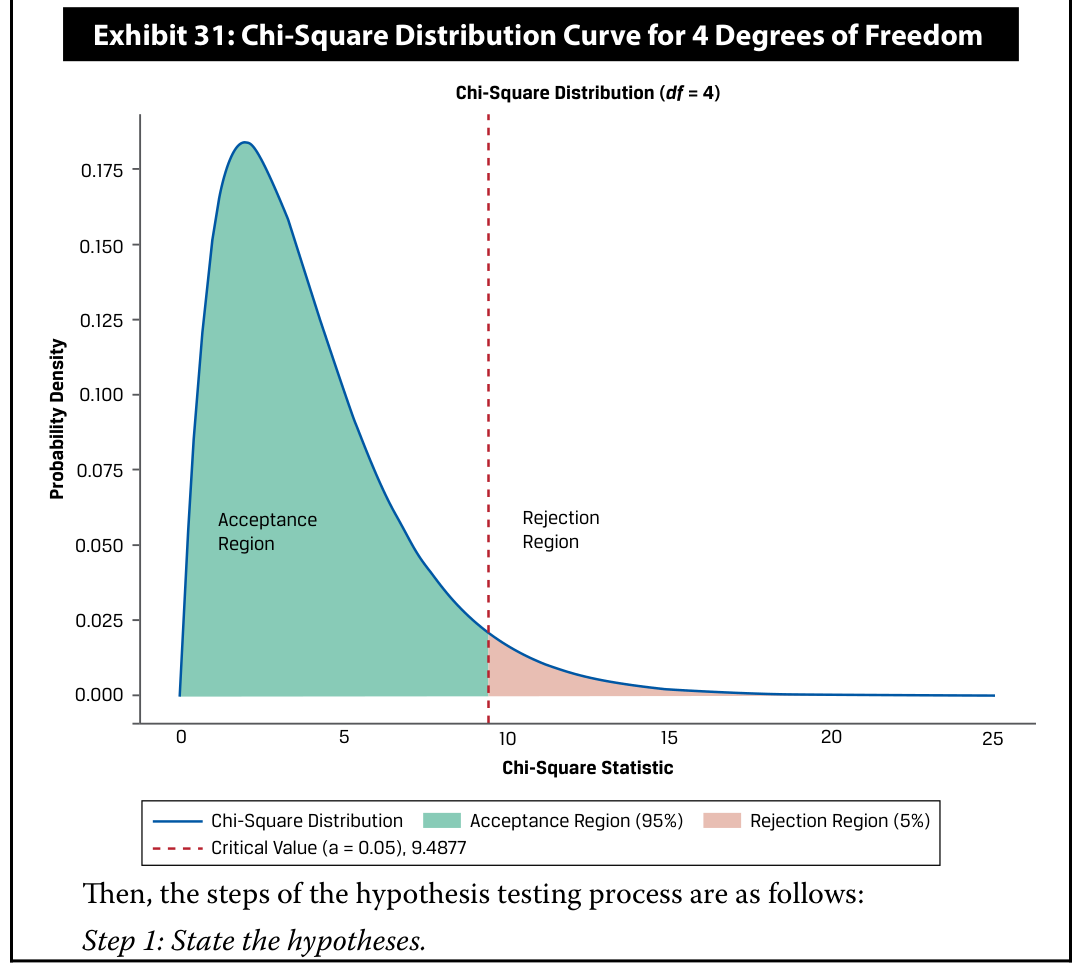
\includegraphics[width=0.75\linewidth]{002_figs/007_Module_7/exhibit_31.png}
	\caption{Chi-Square Distribution Curve with 4 Degrees of Freedom}
	\label{fig:mod7_exhibit_31}
\end{figure}
% Reference: CFA Curriculum 2027, Volume 1, Module 7, Page 375, Exhibit 31

\begin{tcolorbox}[
	colback=gray!5!white,
	colframe=black!15!white,
	boxrule=0.5pt,
	arc=3pt,
	title=\textbf{Case Study: Fund Size and Investment Style of 1,594 ETFs},
	coltitle=black,
	colbacktitle=black!5!white,
	before skip=6pt,
	after skip=6pt,
	breakable
]
We test whether ETF size and investment style are independent (Table~\ref{tab:etf_contingency_m7}). Calculated expected frequencies and scaled squared deviations yield $\chi^2 = 32.07$ (Exhibit~\ref{fig:mod7_exhibit_35}). With $df = 4$, the critical value at 1\% is $13.28$. Since $32.07 > 13.28$, we reject the null hypothesis of independence. 
Analyzing standardized residuals (Exhibit~\ref{fig:mod7_exhibit_36}), the cell for Medium-Growth has a residual of $+3.69$ (significantly higher than expected), and Large-Growth has a residual of $-2.72$ (significantly lower than expected).
\end{tcolorbox}

\begin{table}[!htbp]
\centering
\caption{ETFs Classifications Contingency Table ($N=1,594$)}
\label{tab:etf_contingency_m7}
\begin{tabular}{p{0.25\linewidth} p{0.15\linewidth} p{0.15\linewidth} p{0.15\linewidth} p{0.15\linewidth}}
\toprule
\textbf{Investment Type} & \textbf{Small} & \textbf{Medium} & \textbf{Large} & \textbf{Total} \\
\midrule
\textbf{Value} & 50 & 110 & 343 & 503 \\
\textbf{Growth} & 42 & 122 & 202 & 366 \\
\textbf{Blend} & 56 & 149 & 520 & 725 \\
\midrule
\textbf{Total} & 148 & 381 & 1,065 & 1,594 \\
\bottomrule
\end{tabular}
\end{table}
% Reference: CFA Curriculum 2027, Volume 1, Module 7, Page 377, Exhibit 33

\begin{figure}[!htbp]
	\centering
	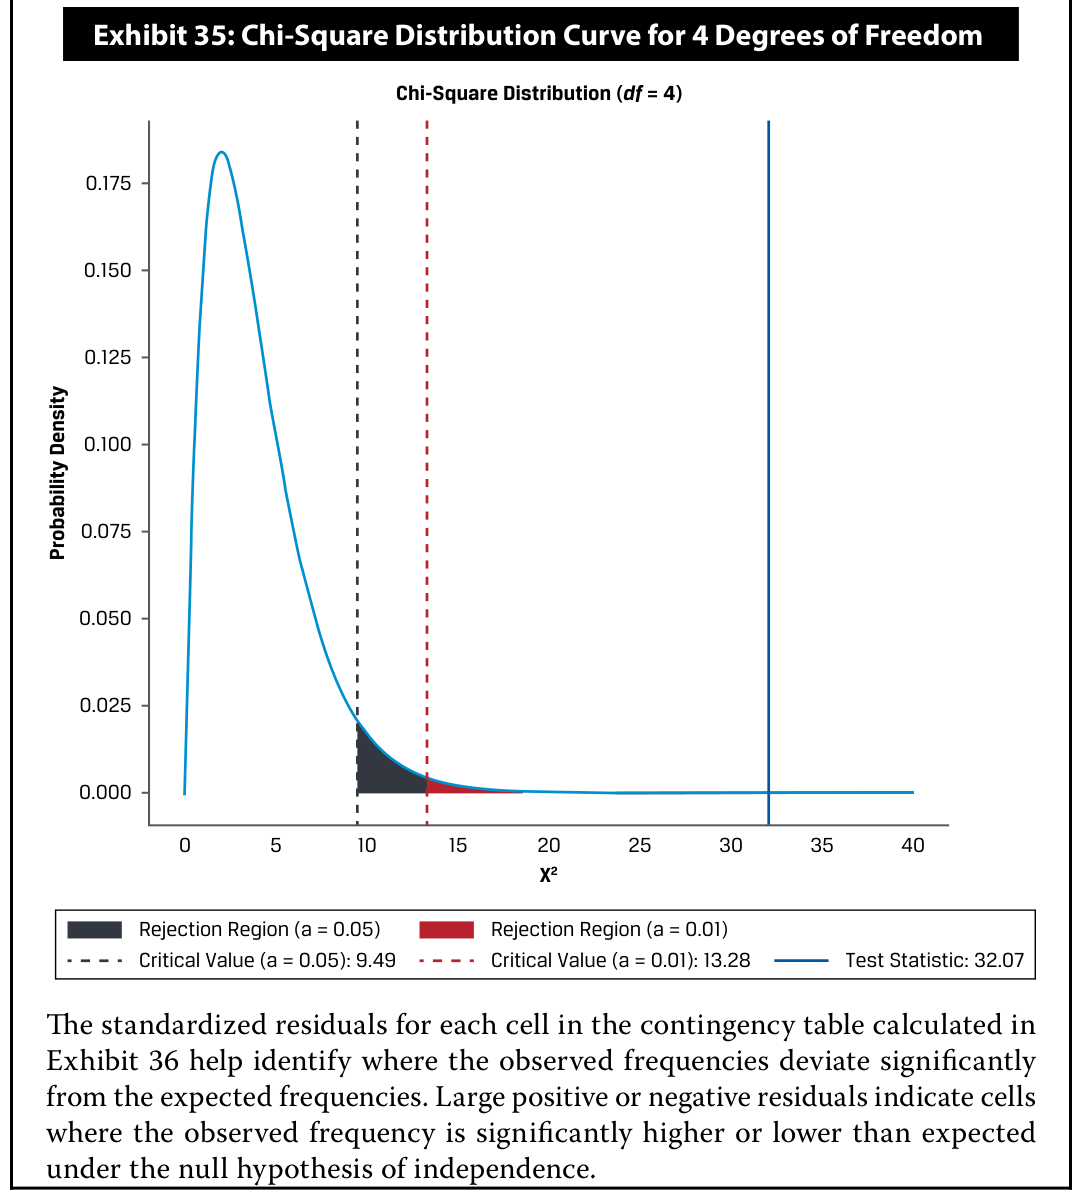
\includegraphics[width=0.75\linewidth]{002_figs/007_Module_7/exhibit_35.png}
	\caption{Chi-Square Rejection Regions for ETF Independence Test ($df=4$)}
	\label{fig:mod7_exhibit_35}
\end{figure}
% Reference: CFA Curriculum 2027, Volume 1, Module 7, Page 379, Exhibit 35

\begin{figure}[!htbp]
	\centering
	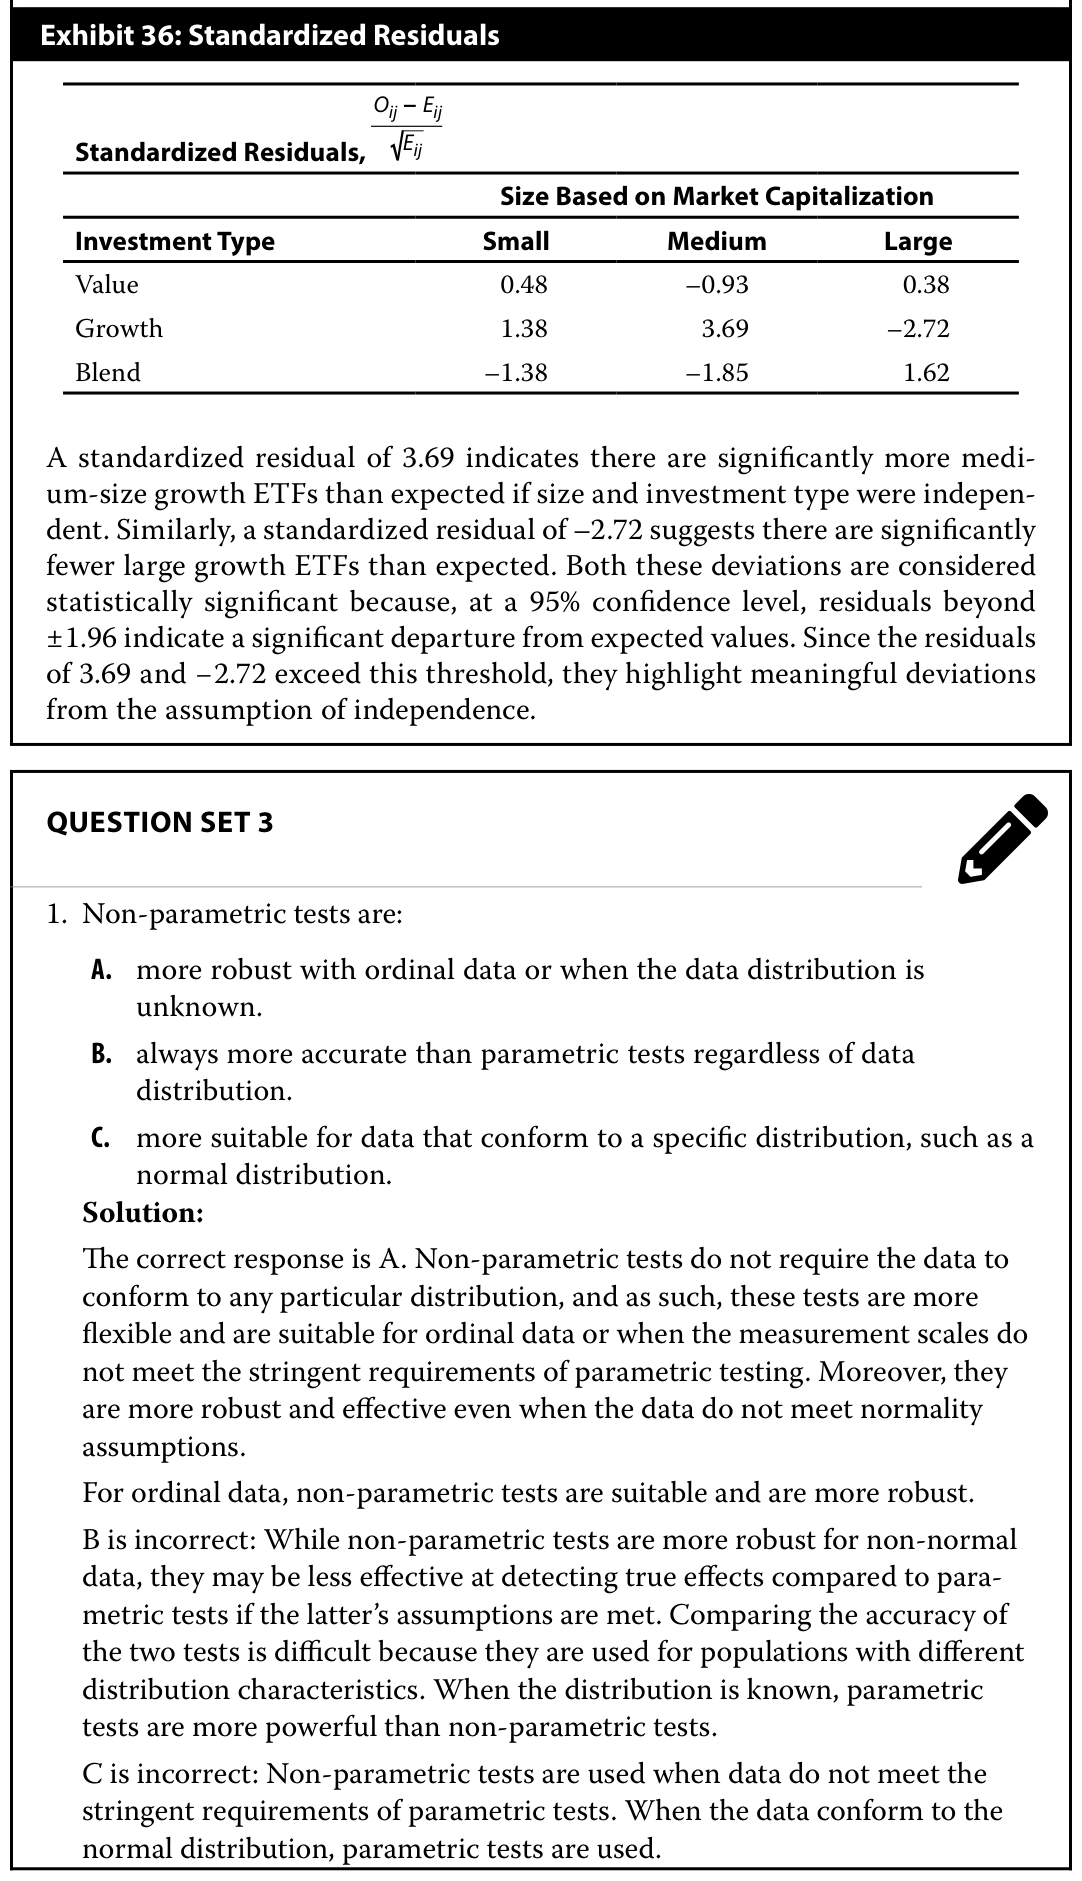
\includegraphics[width=0.75\linewidth]{002_figs/007_Module_7/exhibit_36.png}
	\caption{Standardized Residuals plot for Size vs Style of ETFs}
	\label{fig:mod7_exhibit_36}
\end{figure}
% Reference: CFA Curriculum 2027, Volume 1, Module 7, Page 380, Exhibit 36
 % Estimation and Hypothesis Testing
\chapter{The Return and Risk of a Financial Portfolio}
\label{chap:The Return and Risk of a Financial Portfolio}

\begin{center}
\begin{tabular}{p{0.06\linewidth} | p{0.88\linewidth}}
	\toprule
	\multicolumn{2}{l}{\textbf{LEARNING OUTCOMES}} \\
	\midrule
	a & calculate, interpret, and evaluate the expected return, variance, standard deviation, covariance, and correlation of portfolio returns \\
	\midrule
	b & describe, calculate, and interpret the minimum-variance portfolio and portfolios that lie on the efficient frontier \\
	\midrule
	c & explain the selection of an optimal portfolio, given an investor's risk aversion and the capital allocation line, and how this extends to the market portfolio and the capital market line \\
	\bottomrule
\end{tabular}
\end{center}

\vspace{1em}

\begin{itemize}
	\item[] \textbf{Calculating Portfolio Statistics}
	      \begin{itemize}
			\item[] Returns of a Portfolio
			\item[] Variance and Standard Deviation of Portfolio Returns
			\item[] The Benefits of Diversification
			\item[] Types of Returns: Financial Indicators
			\item[] Long-Term Financial Asset Returns
			\item[] Risks and Returns
	      \end{itemize}
	\item[] \textbf{The Minimum-Variance Portfolio and the Efficient Frontier}
	      \begin{itemize}
			\item[] The Minimum-Variance Portfolio
			\item[] The Minimum-Variance Frontier
			\item[] Portfolio Optimization
	      \end{itemize}
	\item[] \textbf{Optimal Portfolio Selection}
	      \begin{itemize}
			\item[] The Capital Allocation Line (CAL)
			\item[] The Capital Market Line (CML)
			\item[] The Capital Asset Pricing Model (CAPM)
			\item[] Limitations
	      \end{itemize}
\end{itemize}
 % The Return and Risk of a Financial Portfolio
\chapter{Simulation of Financial Asset Prices and Returns}
\label{chap:Simulation of Financial Asset Prices and Returns}

\begin{center}
\begin{tabular}{p{0.06\linewidth} | p{0.88\linewidth}}
	\toprule
	\multicolumn{2}{l}{\textbf{LEARNING OUTCOMES}} \\
	\midrule
	a & describe historical simulation and explain how it can be used in investment applications \\
	\midrule
	b & describe bootstrap resampling, and explain how it can be used in investment applications \\
	\midrule
	c & describe Monte Carlo simulation and explain how it can be used in investment applications \\
	\bottomrule
\end{tabular}
\end{center}

\vspace{1em}

\begin{itemize}
	\item[] \textbf{Historical Simulation}
	      \begin{itemize}
			\item[] Overview of Simulation Methods
			\item[] Historical Simulation Overview
			\item[] Implementing Historical Simulation
			\item[] Features of Historical Simulation
	      \end{itemize}
	\item[] \textbf{Bootstrapping}
	      \begin{itemize}
			\item[] Bootstrapping Overview
			\item[] Implementing Bootstrapping
			\item[] Features of Bootstrapping Simulations
	      \end{itemize}
	\item[] \textbf{Monte Carlo Simulation}
	      \begin{itemize}
			\item[] Monte Carlo Simulation Overview
			\item[] Multivariate Monte Carlo Simulation
			\item[] Features of Monte Carlo Simulation
			\item[] Practical Implementation of Simulation Approaches Using Excel and Other Tools
	      \end{itemize}
\end{itemize}
 % Simulation of Financial Asset Prices and Returns
\chapter{Applications of Simple Linear Regression in Finance}
\label{chap:Applications of Simple Linear Regression in Finance}

\begin{center}
\begin{tabular}{p{0.06\linewidth} | p{0.88\linewidth}}
	\toprule
	\multicolumn{2}{l}{\textbf{LEARNING OUTCOMES}} \\
	\midrule
	a & describe, interpret, and explain simple linear regression, including coefficient estimation using the least squares criterion \\
	\midrule
	b & describe and compare the assumptions of simple linear regression, identify violations through analyzing residuals, evaluate the estimated mode's goodness-of-fit and regression coefficients, and results of ANOVA estimates \\
	\midrule
	c & calculate and interpret predicted values, the standard error of the estimate, and prediction intervals for the dependent variable in a simple linear regression model and describe different functional forms \\
	\midrule
	d & calculate and interpret the variable estimates of the capital asset pricing model (CAPM) \\
	\bottomrule
\end{tabular}
\end{center}

\vspace{1em}

\begin{itemize}
	\item[] \textbf{Linear Regression Estimation}
	      \begin{itemize}
			\item[] Linear Regression Analysis
			\item[] Coefficient Estimation of Linear Regression
			\item[] Estimation Residuals
			\item[] Data Types
	      \end{itemize}
	\item[] \textbf{Limitations of Linear Regression Models}
	      \begin{itemize}
			\item[] Assumptions of the Simple Linear Regression Model
			\item[] Residual Analysis
			\item[] Evaluating Goodness-of-Fit and Regression Coefficients
			\item[] Hypothesis Testing
	      \end{itemize}
	\item[] \textbf{Using Linear Regression Models for Prediction}
	      \begin{itemize}
			\item[] Prediction Using a Simple Regression
			\item[] Modeling Non-Linear Relationships in Economic and Financial Data
			\item[] Practical Implementation
			\item[] Hypothesis Testing
	      \end{itemize}
	\item[] \textbf{Using Linear Regression Models to Evaluate Financial Assets: The Capital Asset Pricing Model}
\end{itemize}
 % Applications of Simple Linear Regression in Finance
\chapter{Introduction to Financial Data Science}
\label{chap:Introduction to Financial Data Science}

\begin{center}
\begin{tabular}{p{0.06\linewidth} | p{0.88\linewidth}}
	\toprule
	\multicolumn{2}{l}{\textbf{LEARNING OUTCOMES}} \\
	\midrule
	a & describe how big data, machine learning, and artificial intelligence are used in financial data science, fintech, and investment management \\
	\bottomrule
\end{tabular}
\end{center}

\vspace{1.5em}

\section{Financial Data and Big Data}
\label{sec:Financial Data and Big Data}

\textcolor{blue}{\textit{Dữ liệu định lượng (quantitative) như giá cả, lợi suất đã rất quen thuộc. Nhưng cuộc cách mạng thực sự nằm ở dữ liệu định tính (qualitative) và dữ liệu thay thế (alternative data). Nhờ sự phát triển của công nghệ số, chúng ta có thể chuyển hóa các cuộc gọi thu nhập, tin tức hay bài đăng mạng xã hội thành số liệu để phân tích đồng thời. Hãy suy nghĩ: dữ liệu nào sẽ mang lại lợi thế cạnh tranh lớn hơn trong tương lai?}}

\subsection{Quantitative vs. Qualitative Data}
The investment decision-making process analyzes both quantitative and qualitative data:
\begin{itemize}
	\item \textbf{Quantitative data} describes numeric information, such as prices, returns, interest rates, currency exchange rates, economic indicators, and accounting numbers, that can be analyzed using statistical methods.
	\item \textbf{Qualitative data} describes non-numeric information, such as market sentiment, management quality, industry trends, environmental factors (ESG), and geopolitical risks.
\end{itemize}
With the advance of digitization, qualitative data are increasingly captured digitally and processed algorithmically (e.g., using sentiment analysis), allowing for the integration of qualitative insights with quantitative analysis.

\subsection{Characteristics of Big Data (The 4 Vs)}
Datasets available for analysis are growing rapidly. Big data are characterized by four key dimensions:
\begin{itemize}
	\item \textbf{Volume:} The vast amount of data collected (ranging from megabytes to gigabytes, terabytes, and petabytes), representing millions or billions of observations.
	\item \textbf{Velocity:} The speed at which data are communicated and updated. Real-time or low-latency data feeds have become the standard in financial applications.
	\item \textbf{Variety:} The diversity of data formats and sources, which can be structured, semi-structured, or unstructured.
	\item \textbf{Veracity:} The credibility, authenticity, and reliability of different data sources. Veracity is critical in big data because of the varying quality of large, non-traditional datasets.
\end{itemize}

\begin{figure}[!htbp]
	\centering
	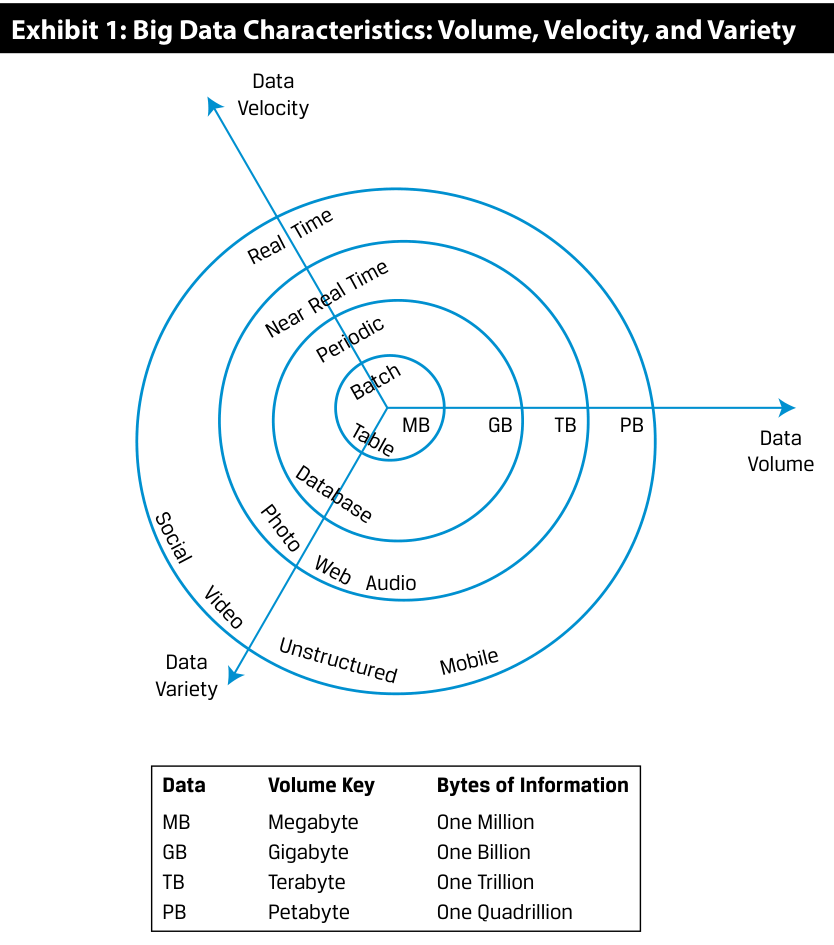
\includegraphics[width=0.75\linewidth]{002_figs/011_Module_11/11.1-Big Data Characteristics.png}
	\caption{Characteristics of Big Data: Volume, Variety, and Velocity}
	\label{fig:big_data_characteristics}
\end{figure}

\subsection{Data Types and Sources}
Data can be classified into three types based on structure:
\begin{itemize}
	\item \textbf{Structured data:} Organized in tables (rows and columns) and commonly stored in databases where fields are defined (e.g., SQL tables, CSV files).
	\item \textbf{Unstructured data:} Disparate, unorganized data that do not fit into traditional tables. Examples include social media posts, emails, voice recordings, pictures, and video feeds.
	\item \textbf{Semi-structured data:} Blends structured and unstructured elements. The data do not fit into traditional tables but contain tags or markers (e.g., HTML/XML code, JSON files, tagged financial news).
\end{itemize}

Table~\ref{tab:big_data_sources} outlines common sources of big data in finance:

\begin{table}[!htbp]
\centering
\caption{Examples of Big Data Sources in Finance}
\label{tab:big_data_sources}
\begin{tabular}{p{0.25\linewidth} | p{0.65\linewidth}}
	\toprule
	\textbf{Source} & \textbf{Examples} \\
	\midrule
	Financial markets & Equity, fixed income, futures, options, other derivatives, and commodities. \\
	Businesses & Corporate financial statements, commercial transactions, credit card purchases, and supply chain data. \\
	Governments & Trade, economic indicators, regulatory filings, taxation, and payroll data. \\
	Individuals & Personal websites, online product reviews, internet search logs, email, and social media posts. \\
	Sensors & Satellite imagery, aircraft tracking, shipping cargo data, and vehicle traffic patterns. \\
	Internet of Things & Data from smart buildings (climate control, energy usage) and connected commercial devices. \\
	\bottomrule
\end{tabular}
\end{table}

\subsection{Alternative Data and Risks}
\textbf{Alternative data} refers to information collected from non-traditional sources, such as satellite imagery, web traffic, social media sentiment, mobile device geolocation, and retail point-of-sale scanners.
\begin{itemize}
	\item \textbf{Data generated by individuals:} Personal activities like social media clicks, product reviews, and web searches. This data tends to be unstructured and qualitative.
	\item \textbf{Data generated by business processes:} Direct transactions like credit card purchases or point-of-sale scanner data. This structured data acts as a leading indicator of performance, whereas traditional corporate filings are lagging indicators.
	\item \textbf{Data generated by sensors:} Satellite imagery (e.g., counting cars in retail parking lots to predict earnings or monitoring flare gas at oil rigs) and Internet of Things (IoT) streams. It is largely unstructured and grows exponentially.
\end{itemize}

\textcolor{blue}{\textit{Lưu ý về đạo đức và pháp lý: Việc khai thác dữ liệu từ các trang web (Web scraping) có thể vi phạm các quy định bảo mật thông tin cá nhân (GDPR) hoặc bản quyền điều khoản dịch vụ của bên sở hữu dữ liệu. Khi các mô hình đầu tư phụ thuộc nhiều vào dữ liệu phi chính thống, tính tuân thủ pháp lý của nguồn dữ liệu trở thành yếu tố sống còn.}}

\vspace{1.5em}

\section{Financial Data Science and Fintech}
\label{sec:Financial Data Science and Fintech}

\subsection{Definitions}
\begin{itemize}
	\item \textbf{Data science} is an interdisciplinary field combining statistical methods, mathematical models, computational tools, and domain-specific knowledge to clean, process, and interpret big data.
	\item \textbf{Financial data science} applies data science principles specifically to financial datasets (prices, interest rates, returns, accounting statements, and macroeconomic variables) to support investment, portfolio management, trading, and risk decisions.
\end{itemize}

\subsection{Unique Characteristics of Financial Data}
Financial data exhibits unique challenges that require specialized analytical tools:
\begin{enumerate}
	\item \textbf{High volume and speed:} Market transactions occur in microseconds, producing a massive continuous stream of tick data.
	\item \textbf{Sequential and time-dependent structure:} Observations are chronologically ordered, requiring time-series analysis rather than standard independent assumptions.
	\item \textbf{Noise and non-stationarity:} Financial data are highly noisy (containing random fluctuations) and non-stationary (statistical properties like mean and variance change over time).
	\item \textbf{Interdependencies and non-linearity:} Financial variables have complex, non-linear relationships. Advanced tools like \textbf{Copulas} (mathematical functions joining multivariate distributions to capture dependency structures) and neural networks are used.
	\item \textbf{Seasonal and cyclic patterns:} Recurring periods, such as quarterly corporate earnings releases or macro business cycles.
	\item \textbf{Extreme events and fat tails:} Returns exhibit fat-tailed distributions, meaning extreme market crashes or jumps occur far more frequently than predicted by a standard Gaussian distribution.
	\item \textbf{Data sparsity and missing values:} Emerging markets or private assets often lack complete historical data, requiring robust imputation methods to avoid estimation bias.
\end{enumerate}

\subsection{Fintech Evolution}
\textbf{Fintech} (financial technology) represents technological innovation in the design and delivery of financial services and products.
It has evolved through several stages:
\begin{itemize}
	\item \textbf{Early stage:} Routine automation and simple data processing (e.g., calculating bookkeeping records).
	\item \textbf{Intermediate stage:} Rule-based decision execution systems ("if-then" systems).
	\item \textbf{Advanced stage:} Complex algorithmic and machine learning decision-making (e.g., robo-advisors that automatically construct, balance, and manage diversified portfolios based on client risk profiles and target return requirements).
\end{itemize}

\vspace{1.5em}

\section{Machine Learning and Artificial Intelligence}
\label{sec:Machine Learning and Artificial Intelligence}

\textcolor{blue}{\textit{Trong học máy, triết lý cốt lõi là ``find the pattern, apply the pattern'' (tìm kiếm mẫu và áp dụng mẫu). Thay vị con người phải lập trình từng dòng quy tắc, thuật toán tự rút ra cấu trúc ẩn của dữ liệu từ quá trình huấn luyện (training). Hãy nắm chắc cách phân chia tập dữ liệu và sự khác biệt giữa các phương pháp học để trả lời chính xác câu hỏi trong kỳ thi.}}

\subsection{Dataset Splitting and Time-Series Validation}
In machine learning (ML), datasets are divided into three distinct subsets:
\begin{itemize}
	\item \textbf{Training dataset:} The largest portion (typically 60\%--80\%) used by the algorithm to identify historical relationships between inputs and targets.
	\item \textbf{Validation dataset:} Used to validate and tune the model's parameters and refine its performance (10\%--20\%).
	\item \textbf{Testing dataset:} Used at the very end to evaluate the model's performance on unseen, out-of-sample data (10\%--20\%).
\end{itemize}

For cross-sectional data, data is split randomly. This randomization prevents bias and helps prevent \textbf{data leakage} (when information from outside the training set accidentally influences the model).
For time-series data, simple randomization cannot be used because it disrupts the chronological sequence and introduces forward data leakage (predicting the past using future data). Instead, analysts use:
\begin{itemize}
	\item \textbf{Time-based splits:} Earlier data is allocated to the training set and subsequent chronological blocks are used for validation and testing.
	\item \textbf{Rolling-window validation:} Shifts a fixed-size historical window forward in time, training on one window and validating on the next sequential period.
\end{itemize}

\begin{figure}[!htbp]
	\centering
	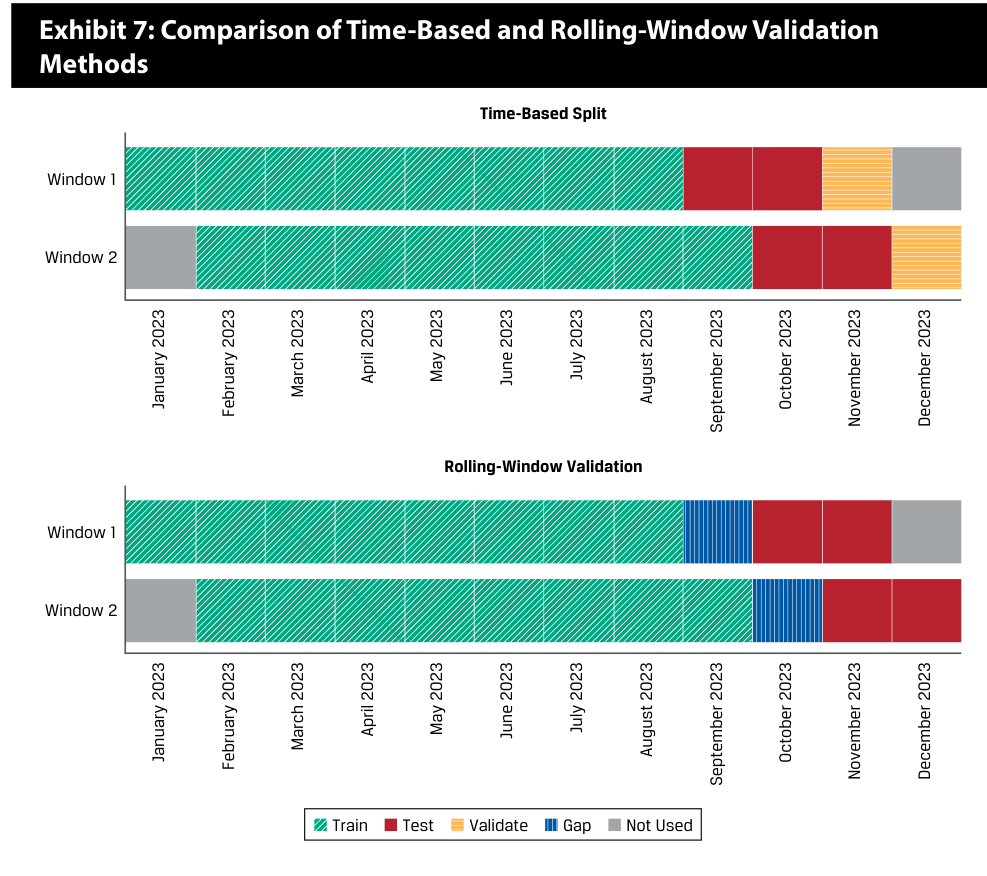
\includegraphics[width=0.8\linewidth]{002_figs/011_Module_11/11.2-Time vs Rolling.png}
	\caption{Time-Based Split vs. Rolling-Window Validation}
	\label{fig:time_vs_rolling}
\end{figure}

\subsection{Overfitting vs. Underfitting}
\begin{itemize}
	\item \textbf{Overfitting:} The model learns the training data too precisely, capturing random noise as if it were a true parameter. This leads to extremely low training error but high out-of-sample test error ($Error_{\text{train}} \ll Error_{\text{test}}$).
	\item \textbf{Underfitting:} The model is too simplistic and treats true relationships as noise, failing to learn the underlying structure in the training data.
\end{itemize}

\subsection{Machine Learning Approaches}
Machine learning is classified into four main approaches, summarized in Table~\ref{tab:ml_approaches}:

\begin{table}[!htbp]
\centering
\caption{Comparison of Machine Learning Approaches}
\label{tab:ml_approaches}
\begin{tabular}{p{0.14\linewidth} | p{0.22\linewidth} | p{0.15\linewidth} | p{0.16\linewidth} | p{0.16\linewidth}}
	\toprule
	\textbf{Approach} & \textbf{Description} & \textbf{Applications} & \textbf{Advantages} & \textbf{Limitations} \\
	\midrule
	\textbf{Supervised learning} & Models learn from labeled historical training data where target output is known. & • Spam detection \newline • Stock return prediction \newline • Default classification & • Highly accurate \newline • Well-understood methods & • Labeled data is costly \newline • Fails to generalize to new scenarios \\
	\midrule
	\textbf{Unsupervised learning} & Models analyze unlabeled data to discover hidden structures and groupings. & • Customer segmentation \newline • Anomaly detection \newline • Dimension reduction & • Discovers unexpected patterns \newline • Reduces data dimensionality & • Subjective evaluation \newline • Difficult to interpret results \\
	\midrule
	\textbf{Reinforcement learning} & Models learn by trial-and-error interaction with an environment to maximize rewards. & • Portfolio optimization \newline • Algorithmic execution & • Good for sequential decisions \newline • Adapts to dynamics & • High training time \newline • Sensitive to reward design \\
	\midrule
	\textbf{Deep learning} & Models use multi-layered artificial neural networks to extract abstract patterns. & • Image recognition \newline • NLP & • Automatically extracts features \newline • Models non-linear structures & • "Black box" nature \newline • Requires massive datasets \\
	\bottomrule
\end{tabular}
\end{table}

\subsection{Neural Networks and Generative Models}
\textbf{Neural networks} are computational models inspired by biological brains. A neural network consists of layers of interconnected nodes (neurons):
\begin{itemize}
	\item \textbf{Input layer:} Receives the raw input features (e.g., historical returns, financial ratios).
	\item \textbf{Hidden layers:} Intermediate layers where non-linear data transformations occur. Multiple hidden layers constitute a "deep" neural network.
	\item \textbf{Output layer:} Provides the final classification or predicted continuous value.
\end{itemize}

\begin{figure}[!htbp]
	\centering
	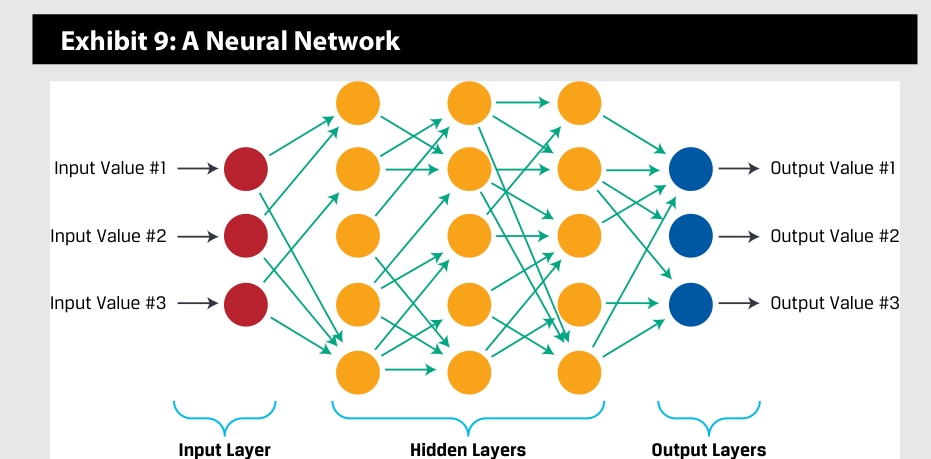
\includegraphics[width=0.7\linewidth]{002_figs/011_Module_11/11.3-Neural Network.png}
	\caption{Structure of an Artificial Neural Network}
	\label{fig:neural_network}
\end{figure}

Training is completed using **backpropagation**:
1. \textbf{Forward pass:} Data flows through the network to generate a prediction.
2. \textbf{Loss calculation:} Computes the error (loss) between the predicted and actual target.
3. \textbf{Backward pass (Backpropagation):} Calculates gradients of the loss function with respect to the network weights.
4. \textbf{Weight update:} Weights are updated slightly in the opposite direction of the gradient using **gradient descent**.
This process is repeated over multiple cycles (**epochs**) until the network converges.

Two advanced generative neural network architectures are:
\begin{itemize}
	\item \textbf{Generative Adversarial Networks (GANs):} Combines a generator network (creates synthetic data) and a discriminator network (evaluates authenticity) in an adversarial loop. Used to generate synthetic financial scenarios for stress-testing.
	\item \textbf{Variational Autoencoders (VAEs):} Compresses inputs into a latent, lower-dimensional space (encoder) and reconstructs them (decoder). Useful for dimensionality reduction and anomaly detection.
\end{itemize}

\vspace{1.5em}

\section{Natural Language Processing and Generative AI}
\label{sec:NLP and Generative AI}

\subsection{Natural Language Processing (NLP)}
\begin{itemize}
	\item \textbf{Text analytics} extracts information and identifies patterns from unstructured text- or voice-based datasets (filings, transcripts, emails, news, etc.).
	\item \textbf{Natural language processing (NLP)} is a subfield at the intersection of computer science, AI, and linguistics focused on analyzing human language.
\end{itemize}
Common applications in finance include sentiment analysis (e.g., parsing earnings call transcripts to assign a positive/negative sentiment rating to detect subtle manager outlooks before analyst rating updates) and monitoring central bank communication (parsing Fed or ECB statements to extract tone shifts on interest rates).

\subsection{Large Language Models (LLMs)}
**Large Language Models (LLMs)**, such as GPT models, represent a significant advancement in generative AI. 
\begin{itemize}
	\item \textbf{Architecture:} Rely on **transformers** to process and capture long-range contextual relationships within textual sequences.
	\item \textbf{Huấn luyện song miền (Dual-domain training):} Sourced via self-supervised learning on massive general corpora (to learn grammar, semantics) and specialized financial corpora (filings, earnings call transcripts to master domain jargon).
	\item \textbf{Tinh chỉnh (Fine-tuning):} Adapted via transfer learning for specialized applications (e.g., text generation, report summarization, financial sentiment analysis).
	\item \textbf{Rủi ro và hạn chế (Risks):} LLMs excel at language prediction but are prone to **hallucinations** (generating false information) and lack numerical calculation capabilities. Over-reliance can result in strategic and regulatory errors. A hybrid model combining automated outputs with human review is recommended.
\end{itemize}

\subsection{Generative AI vs. Traditional Simulations}
**Generative AI** creates new content or scenarios based on representations learned during training. Unlike Monte Carlo simulations (which assume predefined parametric distributions) or bootstrapping (which simply shuffles or resamples historical records), Generative AI learns complex underlying data structures to produce realistic, non-replication-constrained synthetic scenarios.

\vspace{1.5em}

\section{Practice Problems and Solutions}
\label{sec:Practice_Problems_Module_11}
\textcolor{blue}{\textit{Các bài tập ôn tập kèm Lời giải của Module 11 đã được chuyển về Chương 14 (Bài tập ôn tập và Lời giải) ở cuối bản PDF để tiện tra cứu tập trung. Xem bài tập và lời giải tại trang \pageref{sec:app_Problems_M11}.}}
 % Introduction to Financial Data Science

\begin{appendix}
    \listoftables
    \listoffigures
\end{appendix}

\end{document}
